\documentclass[11pt,a4paper]{article}
\usepackage[margin=1in]{geometry}
\usepackage{amsmath,amssymb,amsthm,mathtools}
\usepackage{enumitem}
\usepackage{graphicx}
\usepackage{xcolor}
\usepackage{hyperref}
\usepackage{booktabs}
\usepackage{siunitx}
\usepackage{pgfplots}
\pgfplotsset{compat=1.18}
\usepgfplotslibrary{statistics}
\usetikzlibrary{patterns}

% \quid as environment supports multiple paragraphs and displayed math
\makeatletter
\long\def\quid#1{\begingroup\color{blue}\itshape #1\endgroup}
\makeatother

\title{Take Home -- Advanced Microeconomics\\[0.25em]\large Solutions}
\author{Alessandro Caggia}
\date{May 2026}

\begin{document}
\maketitle

%====================================================================
\section*{Problem 1: Overworked Americans}
%====================================================================

\subsection*{Q1 -- Documenting the US--Europe hours gap}

\paragraph{The headline fact.}
Per working-age adult (15--64), the United States supplies roughly \textbf{25\% more annual market hours} than Germany or France. The gap is large (an order of magnitude bigger than typical business-cycle fluctuations), \emph{recent} (fully absent in 1970), and \emph{mostly intensive-margin} --- driven by weeks worked per year, not the employment rate.

\paragraph{Accounting identity.}
I decompose total market hours per working-age adult into four multiplicative components:
\begin{equation}
\underbrace{\frac{H}{N}}_{\text{hours / adult}}
\;=\;\underbrace{\frac{L}{N}}_{\text{LFPR}}\,\cdot\,
\underbrace{\frac{E}{L}}_{1-u\text{ (employment)}}\,\cdot\,
\underbrace{D}_{\text{weeks / year}}\,\cdot\,
\underbrace{h}_{\text{hours / week}}.
\label{eq:decomp}
\end{equation}
Taking logs, each cross-country log-difference $\Delta\ln(H/N)$ is the sum of four additive contributions. This is the natural decomposition for Ohanian--Raffo--Rogerson (2008, \emph{JME}) and Rogerson (2006, \emph{JME}).

\paragraph{Current cross-section.}
OECD \emph{Labour Force Statistics}, 2023 values (or most recent available).

\begin{center}
\footnotesize
\begin{tabular}{lccccc}
\toprule
Country & Hrs/worker & Emp/pop (15--64) & Hrs/adult (15--64) & Weekly hrs & Weeks/year \\
\midrule
United States   & 1\,811 & 0.716 & 1\,297 & 38.7 & 46.8 \\
Germany         & 1\,343 & 0.771 & 1\,036 & 34.7 & 38.7 \\
France          & 1\,500 & 0.685 & 1\,028 & 36.8 & 40.8 \\
Italy           & 1\,734 & 0.617 & 1\,070 & 35.6 & 48.7 \\
United Kingdom  & 1\,524 & 0.753 & 1\,147 & 36.4 & 41.9 \\
Netherlands     & 1\,435 & 0.817 & 1\,172 & 31.4 & 45.7 \\
Sweden          & 1\,440 & 0.775 & 1\,116 & 36.2 & 39.8 \\
Spain           & 1\,644 & 0.654 & 1\,075 & 36.7 & 44.8 \\
Greece          & 1\,886 & 0.622 & 1\,173 & 39.4 & 47.9 \\
Poland          & 1\,815 & 0.702 & 1\,274 & 39.5 & 45.9 \\
\bottomrule
\end{tabular}
\end{center}

\paragraph{Quantitative decomposition of the US--Germany gap.}
Applying \eqref{eq:decomp} to the US vs.\ Germany, with $\Delta\ln(H/N)=\ln(1297/1036)=+0.225$:
\begin{center}
\footnotesize
\begin{tabular}{lrr}
\toprule
Component & Log-difference $\Delta\ln(\cdot)$ & Share of total gap \\
\midrule
Weekly hours $h$ (38.7 vs 34.7) & $+0.109$ & $+48\%$ \\
Weeks per year $D$ (46.8 vs 38.7) & $+0.190$ & $+84\%$ \\
Employment rate $E/N$ (0.716 vs 0.771) & $-0.074$ & $-33\%$ \\
\midrule
Total $\Delta\ln(H/N)$ & $+0.225$ & $100\%$ \\
\bottomrule
\end{tabular}
\end{center}
\emph{Weeks per year is the single largest driver.} Weekly hours add about half again as much. The employment rate partially offsets --- Germany has higher $E/N$ than the US, so a pure ``Americans work, Europeans don't'' narrative is wrong on the extensive margin. The gap lives in how much time the employed Americans spend at work, not whether they are employed.

\paragraph{Historical pattern.}
In 1970, annual hours per worker were essentially \emph{identical} across the Atlantic (all near 1\,900). Hours per worker then fell sharply in Continental Europe during 1970--2000, while US hours stayed roughly flat. Figure~\ref{fig:hoursTS} plots the divergence using OECD data updated with Ohanian--Raffo--Rogerson (2008) for the early decades. The timing matters for modelling: \emph{any} valid theory must explain a \emph{divergence}, not a level difference rooted in deep cultural constants.

\begin{figure}[ht]
\centering
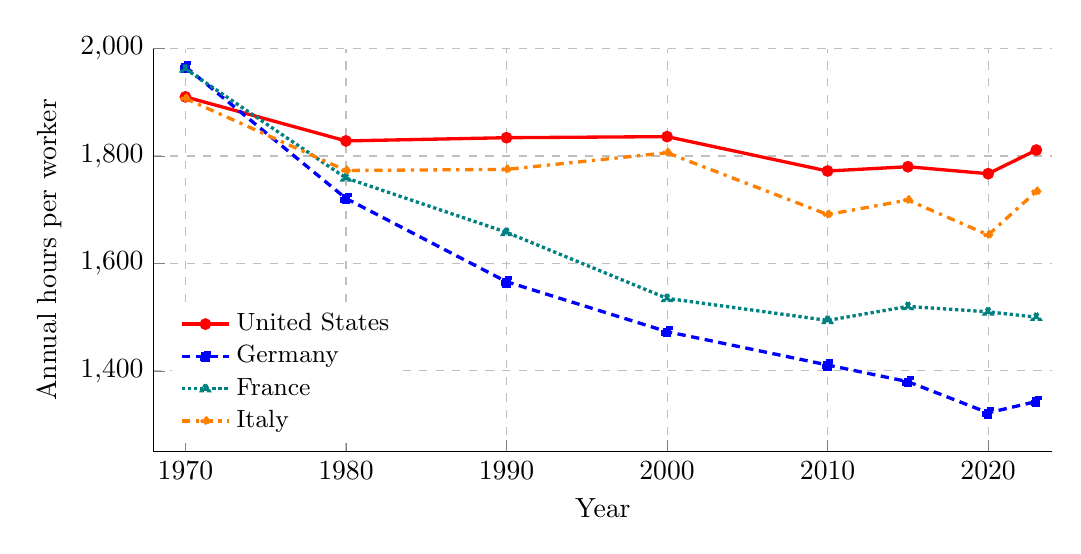
\begin{tikzpicture}
\begin{axis}[
    width=13cm, height=6.7cm,
    xlabel={Year},
    ylabel={Annual hours per worker},
    xmin=1968, xmax=2024, ymin=1250, ymax=2000,
    grid=major, grid style=dashed,
    axis y line*=left, axis x line*=bottom,
    legend style={at={(0.02,0.02)},anchor=south west,draw=none,font=\small,cells={anchor=west}},
    xtick={1970,1980,1990,2000,2010,2020},
    xticklabel style={/pgf/number format/1000 sep={}},
    scaled x ticks=false
]
\addplot[red,very thick,mark=*,mark size=1.5pt] coordinates {
    (1970,1910) (1980,1828) (1990,1834) (2000,1836) (2010,1772) (2015,1780) (2020,1767) (2023,1811)
};
\addlegendentry{United States}
\addplot[blue,very thick,mark=square*,mark size=1.5pt,densely dashed] coordinates {
    (1970,1966) (1980,1721) (1990,1566) (2000,1473) (2010,1411) (2015,1380) (2020,1322) (2023,1343)
};
\addlegendentry{Germany}
\addplot[teal,very thick,mark=triangle*,mark size=1.5pt,densely dotted] coordinates {
    (1970,1962) (1980,1759) (1990,1658) (2000,1535) (2010,1494) (2015,1520) (2020,1510) (2023,1500)
};
\addlegendentry{France}
\addplot[orange,very thick,mark=diamond*,mark size=1.5pt,dashdotted] coordinates {
    (1970,1907) (1980,1773) (1990,1775) (2000,1806) (2010,1691) (2015,1718) (2020,1653) (2023,1734)
};
\addlegendentry{Italy}
\end{axis}
\end{tikzpicture}
\caption{\small Annual hours per worker, 1970--2023. All four economies worked a similar number of hours in 1970; the gap opened after 1970 and stabilised by 2000. Source: OECD \emph{Labour Force Statistics}; 1970--1990 supplemented by Ohanian, Raffo and Rogerson (2008).}
\label{fig:hoursTS}
\end{figure}

\paragraph{Within-Europe heterogeneity.}
``Europe'' is not a homogeneous object. Annual hours per worker split into three clusters:
\begin{itemize}[leftmargin=*,nosep]
    \item \emph{Germanic / Nordic / French}: 1\,340--1\,510 hours (Germany, Denmark, Norway, Netherlands, Sweden, France). The entire headline gap lives here.
    \item \emph{Anglo / Mediterranean}: 1\,500--1\,745 hours (UK, Italy, Spain, Portugal). Intermediate.
    \item \emph{Southern / Eastern}: 1\,700--1\,900 hours (Greece, Poland, Czech Republic, Hungary, Romania). Often at or above the US level.
\end{itemize}
A pure ``institutional Europe vs.\ flexible America'' story therefore fails: high-tax Italy works US-like hours, and Poland --- a mid-tax, post-transition economy --- works the same hours as Texas.

\paragraph{Demographic concentration of the gap.}
Using HETUS and ATUS microdata, Rogerson (2008, \emph{JPE}) and Bick--Br\"uggemann--Fuchs-Sch\"undeln (2019, \emph{JEEA}) find that the US--Germany/France gap is disproportionately located in:
\begin{itemize}[leftmargin=*,nosep]
    \item \emph{Vacation weeks}: statutory paid leave is 10--15 days in the US versus 25--30 in Continental Europe, plus additional national holidays. This alone closes most of the weeks-per-year margin documented above.
    \item \emph{Married women and secondary earners}: US wives supply 350--500 more annual market hours than German or French wives --- the single largest demographic driver.
    \item \emph{Older workers} (55--64): effective retirement age is 3--5 years earlier in Continental Europe, compressing lifetime market hours.
    \item \emph{Self-employed and managers}: longer weekly hours in the US.
\end{itemize}
Prime-age male employees, in contrast, work near-identical \emph{weekly} hours on both continents; the gap is not a story about hard-charging American men.

\noindent\quid{The ``quid'' --- a numerical preview of the puzzle that will drive Q2--Q3. For any tax-based explanation, one must satisfy
\[
\Delta\ln(H/N)\;=\;\varepsilon_{H}\cdot\Delta\ln(1-\tau),
\]
with $\varepsilon_H$ the aggregate elasticity of hours to the net-of-tax factor. Using the Q2 composite wedges ($\tau^{US}\approx 0.40$, $\tau^{DE}\approx 0.60$), $\Delta\ln(1-\tau)=\ln(0.60/0.40)\approx 0.405$, so matching the observed $\Delta\ln(H/N)\approx 0.225$ requires $\varepsilon_H\approx 0.56$. This is already close to twice the intensive-margin Frisch estimated at the micro level (Chetty--Guren--Manoli--Weber, 2011: $\approx 0.3$). Prescott (2004), using a log utility with a high weight on leisure ($\alpha\!\simeq\!1.5$), instead calibrates an \emph{individual} Frisch near $3$; the order-of-magnitude gap with the micro Frisch is exactly the ``implausibility'' critique that the subsequent literature has had to answer. Documenting the fact is therefore inseparable from flagging that a representative-agent model cannot comfortably rationalise it without either a large aggregation mechanism (Rogerson--Hansen lotteries, home production, life-cycle retirement: Q3) or additional non-tax frictions (regulation, unions, household structure: Q4--Q6).}

%--------------------------------------------------------------------
\subsection*{Q2 -- Taxes, labour supply, and Prescott's condition}

\paragraph{US vs.\ Europe income tax in one picture.}
The quantitative object that matters for labour supply is not the statutory marginal rate of the personal income tax, but the \emph{labour tax wedge}
\[
\tau \;\equiv\; 1 \;-\;\frac{1-\tau_l}{1+\tau_c},\qquad
(1-\tau)\;=\;\frac{1-\tau_l}{1+\tau_c},
\]
where $\tau_l$ aggregates personal income tax and (employee + employer) social-security contributions on labour, and $\tau_c$ is the effective consumption tax (VAT/sales). This aggregation matters: a worker supplies labour only in order to consume, so the VAT burden is isomorphic to a labour income tax. Hence the relevant ``tax on work'' is a composite wedge and not the headline marginal rate.

\begin{center}
\small
\begin{tabular}{lcccc}
\toprule
Country & $\tau_l$ (labour wedge, OECD) & Top stat.\ income rate & Std.\ VAT & Composite $\tau$ \\
\midrule
United States   & 0.30 & 0.37 (fed)      & 0.07 (avg.\ sales) & $\approx 0.35$ \\
Germany         & 0.48 & 0.45            & 0.19               & $\approx 0.56$ \\
France          & 0.47 & 0.45            & 0.20               & $\approx 0.56$ \\
Italy           & 0.45 & 0.43            & 0.22               & $\approx 0.55$ \\
Belgium         & 0.53 & 0.50            & 0.21               & $\approx 0.61$ \\
Netherlands     & 0.35 & 0.495           & 0.21               & $\approx 0.46$ \\
United Kingdom  & 0.31 & 0.45            & 0.20               & $\approx 0.42$ \\
Sweden          & 0.42 & $\approx 0.52$  & 0.25               & $\approx 0.54$ \\
\bottomrule
\end{tabular}
\end{center}
\emph{Source: OECD \emph{Taxing Wages} (wedge for a single, average-wage worker, no children, recent years); national tax codes for statutory rates; own calculation of the composite $\tau$ from the formula above using $\tau_l$ and the standard VAT.} The Continental-European composite wedge exceeds the US one by roughly 20 percentage points. Continental Europe also relies more heavily on payroll-financed social-insurance contributions and on VAT; the US instead relies more on (moderately progressive) personal income tax and on less-uniform state-level sales taxes. The \emph{novel} observation at this stage --- novel relative to the purely cross-sectional comparison of statutory rates --- is that after consolidating $\tau_l$ and $\tau_c$ into one composite wedge, the US--Europe distance is \emph{larger} than the distance in income-tax brackets would suggest.

\paragraph{Model of labour supply.}
Representative household with period utility
\begin{equation}
u(c,h)\;=\;\ln c \;+\;\alpha\,\ln(1-h),\qquad \alpha>0,\; h\in[0,1],
\label{eq:utility}
\end{equation}
where $1$ is the time endowment and $h$ is market hours. Wages $w$ are determined by constant-returns technology $y=wh$ and therefore are invariant to the tax; this is the cleanest ``Prescott'' normalisation, designed to isolate the labour-supply margin. Linear taxes $\tau_l$ on labour and $\tau_c$ on consumption; revenues rebated lump-sum, $T$, so the government runs a balanced budget:
\begin{align}
(1+\tau_c)\,c \;&=\;(1-\tau_l)\,w\,h + T, \label{eq:bc}\\
T \;&=\;\tau_l\,w\,h + \tau_c\,c. \label{eq:gbc}
\end{align}
Substituting \eqref{eq:gbc} into \eqref{eq:bc} yields the aggregate resource constraint $c = wh$: \emph{with lump-sum rebating the household's budget in equilibrium is tax-free}. This is critical --- it eliminates the income effect and leaves only a substitution distortion, which is precisely what produces sharp predictions.

The household's FOC, using \eqref{eq:bc} as the constraint faced at the margin (not the one after rebate, since $T$ is lump-sum and therefore taken as given), is
\begin{equation}
\frac{-u_h}{u_c}\;=\;\frac{1-\tau_l}{1+\tau_c}\,w \;\equiv\; (1-\tau)\,w.
\label{eq:foc}
\end{equation}
Plugging \eqref{eq:utility} and equilibrium $c=wh$:
\begin{equation}
\frac{\alpha}{1-h}\cdot wh \;=\; (1-\tau)\,w \;\Longleftrightarrow\; \frac{\alpha\, h}{1-h}\;=\;1-\tau.
\label{eq:implicit}
\end{equation}
Solving for the equilibrium supply of hours:
\begin{equation}
\boxed{\;h^{*}(\tau)\;=\;\frac{1-\tau}{\alpha+(1-\tau)}\;.}
\label{eq:hours}
\end{equation}

\paragraph{Comparative statics and the Prescott condition.}
Differentiating \eqref{eq:hours}:
\begin{equation}
\frac{\partial h^{*}}{\partial \tau}\;=\;-\,\frac{\alpha}{\bigl[\alpha+(1-\tau)\bigr]^{2}}<0,\qquad
\varepsilon_{h,\,1-\tau}\;\equiv\;\frac{\partial\ln h^{*}}{\partial\ln(1-\tau)}\;=\;\frac{\alpha}{\alpha+(1-\tau)}\in(0,1).
\label{eq:elast}
\end{equation}
Hence, hours are strictly decreasing in the composite labour wedge. Since at $c=wh$ the budget is tax-free, the cross-country comparison is driven by pure substitution: a higher $\tau$ reduces the \emph{relative} price of leisure, and hence fewer hours are supplied. Formally, given the Prescott normalisation $w^{US}=w^{EU}$, common preferences, and common lump-sum rebating,
\begin{equation}
\boxed{\;h^{*}(\tau^{EU})<h^{*}(\tau^{US})\;\Longleftrightarrow\;\tau^{EU}>\tau^{US}\;,}
\label{eq:condition}
\end{equation}
and the \emph{sharpness} of the prediction (no wage, no productivity, no income-effect role) follows precisely from the rebate assumption combined with a balanced-growth-preferences specification.

\paragraph{A parametric example (Prescott calibration).}
Take US composite wedge $\tau^{US}=0.40$ and calibrate $\alpha$ so \eqref{eq:hours} matches the US data point $h^{US}=0.33$ (roughly one-third of discretionary time, \emph{Economic Report of the President}, various years):
\[
0.33 \;=\; \frac{0.60}{\alpha+0.60}\;\Longrightarrow\; \alpha \;\approx\; 1.22.
\]
Set $\tau^{EU}=0.60$ as a representative Continental-European value. The model predicts
\[
h^{EU}\;=\;\frac{0.40}{1.22+0.40}\;\approx\;0.247,\qquad
\frac{h^{EU}}{h^{US}}\;\approx\;0.75.
\]
This is close to the empirically observed ratio of annual hours per adult in Germany/France relative to the US documented in Q1 ($\approx 0.78$). The implied labour-supply elasticity at the US point is $\varepsilon_{h,1-\tau}= 1.22/1.82\approx 0.67$.

\begin{figure}[ht]
\centering
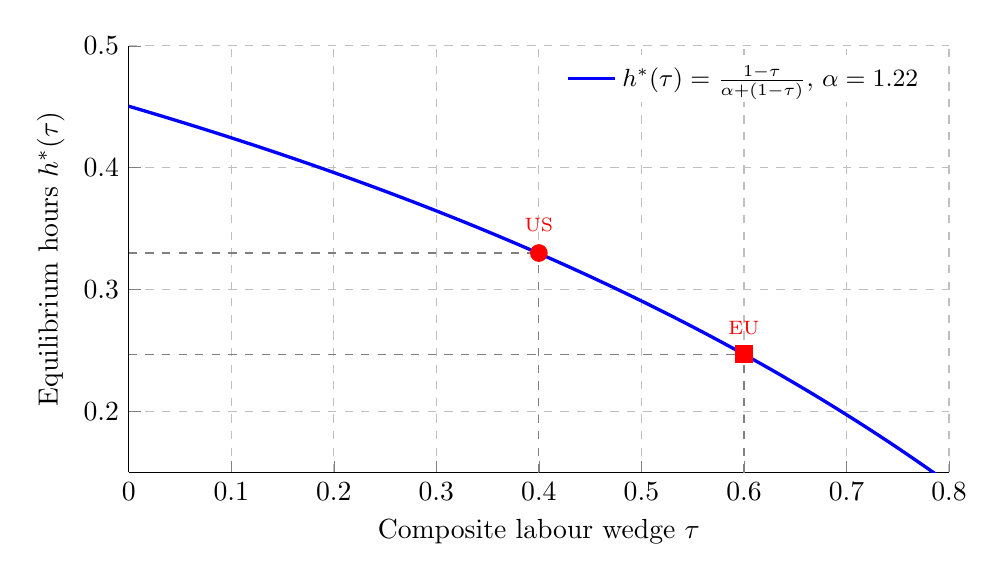
\begin{tikzpicture}
\begin{axis}[
    width=12cm, height=7cm,
    xlabel={Composite labour wedge $\tau$},
    ylabel={Equilibrium hours $h^{*}(\tau)$},
    xmin=0, xmax=0.8, ymin=0.15, ymax=0.5,
    samples=120,
    domain=0:0.8,
    grid=major, grid style=dashed,
    axis y line*=left, axis x line*=bottom,
    legend style={at={(0.98,0.98)},anchor=north east,draw=none,font=\small}
]
\addplot[blue,very thick] {(1-x)/(1.22+1-x)};
\addlegendentry{$h^{*}(\tau)=\frac{1-\tau}{\alpha+(1-\tau)}$, $\alpha=1.22$}

\addplot[red,only marks,mark=*,mark size=3pt] coordinates {(0.40,0.33)};
\node[red,anchor=south] at (axis cs:0.40,0.34) {\scriptsize US};
\addplot[red,only marks,mark=square*,mark size=3pt] coordinates {(0.60,0.247)};
\node[red,anchor=south] at (axis cs:0.60,0.255) {\scriptsize EU};
\draw[gray,dashed] (axis cs:0.40,0) -- (axis cs:0.40,0.33);
\draw[gray,dashed] (axis cs:0.60,0) -- (axis cs:0.60,0.247);
\draw[gray,dashed] (axis cs:0,0.33) -- (axis cs:0.40,0.33);
\draw[gray,dashed] (axis cs:0,0.247) -- (axis cs:0.60,0.247);
\end{axis}
\end{tikzpicture}
\caption{\small Equilibrium hours as a function of the composite wedge $\tau=1-(1-\tau_l)/(1+\tau_c)$. $\alpha$ is calibrated to $h^{US}(\tau^{US}{=}0.40)=0.33$.}
\label{fig:hourstau}
\end{figure}

\paragraph{Summing up.}
Hence, under (i) a representative agent with balanced-growth-compatible preferences, (ii) identical technology across countries, and (iii) balanced-budget lump-sum rebating, higher European labour wedges translate one-to-one into fewer market hours. The condition is simply $\tau^{EU}>\tau^{US}$, and the \emph{size} of the hours gap is governed by $\alpha$ --- the parameter that indexes the preference for leisure or, equivalently, the compensated labour-supply elasticity.

\noindent\quid{The ``quid'' -- three nuances that raise the rigour.

\smallskip
\textbf{(i) Why the rebate matters (and why the income effect vanishes).} Without lump-sum rebating, the budget constraint \eqref{eq:bc} would not collapse to $c=wh$ at the household level, and the comparative statics would involve both a substitution term and an income term of \emph{opposite} sign. With logarithmic utility and no other income, the uncompensated elasticity of hours to the net-of-tax wage is exactly zero (Cobb--Douglas case), and only the rebated-revenue structure produces a non-zero hours response to $\tau$. Making the rebate explicit is therefore not cosmetic: it is the assumption that generates the Prescott effect analytically.

\smallskip
\textbf{(ii) The relevant wedge is composite, not statutory, and is truly novel in its policy implication.} Differentiating the definition,
\[
d\ln(1-\tau)\;=\;-\frac{d\tau_l}{1-\tau_l}\;-\;\frac{d\tau_c}{1+\tau_c}.
\]
Thus a 10 pp rise in VAT and a 10 pp rise in the income-tax rate reduce labour supply by essentially the same amount. Reforms that shift the tax base from income to consumption --- often advocated on efficiency grounds --- have \emph{zero} first-order effect on labour supply in this model, a novel prediction that is often missed in policy debates.

\smallskip
\textbf{(iii) A sharper Prescott condition using the balanced-growth preference class.} If instead of log--log utility one uses the King--Plosser--Rebelo class $u = \tfrac{c^{1-\sigma}}{1-\sigma}v(1-h)$, then equation \eqref{eq:condition} \emph{still holds} for any $\sigma$ with constant Frisch labour supply elasticity, but the \emph{magnitude} of the hours response scales linearly with the Frisch. This localises Prescott's controversy entirely on one parameter --- the Frisch elasticity. Q3 then becomes: how do we justify a \emph{macro} Frisch of order $\ge 1$ while the \emph{micro} Frisch is $\le 0.3$?  That is the natural bridge to the next question.}

%--------------------------------------------------------------------
\subsection*{Q3 -- Why the macro elasticity can exceed the micro one}

\paragraph{The puzzle.} Meta-analyses of micro labour supply (Pencavel 1986; Blundell--MaCurdy 1999; Chetty--Guren--Manoli--Weber 2011, 2012) converge on an intensive-margin Frisch elasticity of $\varepsilon^{\text{int}}\!\approx\!0.1{-}0.3$ for prime-age males and an extensive-margin elasticity of $\varepsilon^{\text{ext}}\!\approx\!0.25$. The Prescott calibration of Q2, in contrast, requires an aggregate elasticity near $\varepsilon^{\text{agg}}\!\approx\!0.7$ (for log utility) or even $\varepsilon^{\text{agg}}\!\approx\!3$ to rationalise the US--Europe gap in \emph{level} terms if wages are held fixed. Hence there is an order-of-magnitude gap between what tax changes do to a single worker's hours and what one would need them to do in the aggregate. The natural rescue is to design a model in which aggregation, not behaviour at the individual margin, produces the elasticity.

\paragraph{A re-written model: indivisible labour with employment lotteries.}
Following Hansen (1985) and Rogerson (1988), postulate that at the individual level labour is \emph{not} a continuous choice but a 0/1 decision. Each worker either supplies a fixed quantity of hours $\bar h$ or zero. The household's problem is then discrete at the individual level but can be convexified through state-contingent employment lotteries.

\smallskip
\emph{Primitives.} Unit continuum of \emph{ex-ante identical} agents; preferences
\begin{equation}
u(c,h)\;=\;\ln c \;-\;\alpha\,\mathbb{1}\{h=\bar h\},\qquad
\bar h\in(0,1),\;\alpha>0.
\label{eq:indiv_util}
\end{equation}
Let $n\in[0,1]$ be the probability of being assigned to ``work'' in the lottery. Conditional on the outcome, consumption is pooled across employed and unemployed agents through complete state-contingent claims. Expected utility of a representative household is
\begin{equation}
\mathcal{U}(c,n)\;=\;\ln c \;-\;\alpha\, n.
\label{eq:agg_util}
\end{equation}
The crucial observation is: although $u$ is non-convex in $h$, $\mathcal{U}$ is \emph{linear} in $n$, so the employment rate becomes a well-defined choice variable and the aggregation is tractable.

\smallskip
\emph{Budget and government.} Linear labour wedge $\tau$ (composite, as in Q2); balanced-budget rebate $T$:
\[
c = (1-\tau)\,w\,\bar h\, n + T,\qquad T = \tau\, w\,\bar h\, n \;\Longrightarrow\; c = w\,\bar h\, n.
\]
Wages pinned down by $y=wh$.

\smallskip
\emph{FOC (taking $T$ as given).} The representative household solves $\max_{c,n}\{\ln c - \alpha n\}$ s.t.\ $c=(1-\tau)w\bar h n + T$. Eliminating $c$:
\begin{equation}
\frac{(1-\tau)w\bar h}{c}\;=\;\alpha
\;\Longrightarrow\; c^{*}\;=\;\frac{(1-\tau)w\bar h}{\alpha}.
\label{eq:foc_indiv}
\end{equation}
Imposing equilibrium $c=w\bar h n$,
\begin{equation}
\boxed{\;n^{*}(\tau)\;=\;\frac{1-\tau}{\alpha},\qquad
H^{*}(\tau)\;=\;n^{*}\bar h \;=\;\frac{(1-\tau)\bar h}{\alpha}\;.}
\label{eq:indiv_hours}
\end{equation}
Hence the aggregate Frisch elasticity is
\begin{equation}
\varepsilon^{\text{agg}}_{H,\,1-\tau}\;=\;\frac{d\ln H^{*}}{d\ln(1-\tau)}\;=\;1,
\label{eq:agg_elast}
\end{equation}
\emph{although the individual intensive-margin elasticity is identically zero}, since any single agent either works $\bar h$ or nothing, independently of $w$ or $\tau$.

\paragraph{Why the two elasticities differ.} The move from the Q2 model to this one replaces the continuous intensive margin with a \emph{participation} margin. Aggregation via lotteries amounts to convexifying the individual choice set. The outcome is that the aggregate function $\mathcal{U}(c,n)$ inherits the \emph{linearity} of the constraint set, while the individual function $u(c,h)$ remains non-convex. This decoupling --- the novel theoretical point first made by Rogerson (1988) --- is what breaks the equivalence between micro and macro Frisch elasticities. A second, equally novel consequence is that micro-econometricians estimating hours regressions on fixed-sample prime-age men are measuring the wrong object: the identification of $\varepsilon^{\text{agg}}$ from panel data requires compositional variation along the extensive margin, which prime-age samples systematically exclude.

\paragraph{Quantitative fit with the US--Europe gap.} With $\tau^{US}=0.40$, $\tau^{EU}=0.60$, the model predicts
\[
\frac{H^{EU}}{H^{US}}\;=\;\frac{1-\tau^{EU}}{1-\tau^{US}}\;=\;\frac{0.40}{0.60}\;=\;0.67.
\]
This overshoots the data ($\approx 0.78$) because \emph{all} the adjustment is extensive-margin. Empirically, the US--EU difference in employment rates is 5--10 pp, not 33 \%, so the pure-lottery model is too strong. The quantitatively successful version combines the intensive Q2 channel with an extensive margin, delivering an aggregate Frisch between $1$ and the micro value --- exactly the empirical range found by Chetty et al.\ (2012).

\begin{figure}[ht]
\centering
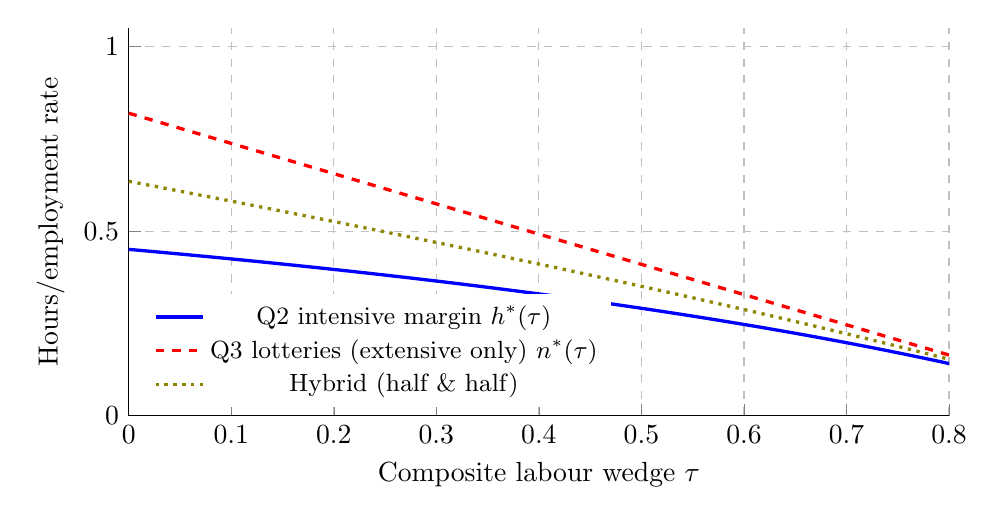
\begin{tikzpicture}
\begin{axis}[
    width=12cm, height=6.5cm,
    xlabel={Composite labour wedge $\tau$},
    ylabel={Hours/employment rate},
    xmin=0, xmax=0.8, ymin=0, ymax=1.05,
    samples=120, domain=0:0.8,
    grid=major, grid style=dashed,
    axis y line*=left, axis x line*=bottom,
    legend style={at={(0.02,0.02)},anchor=south west,draw=none,font=\small}
]
\addplot[blue,very thick] {(1-x)/(1.22+1-x)};
\addlegendentry{Q2 intensive margin $h^{*}(\tau)$}
\addplot[red,very thick,dashed] {(1-x)/1.22};
\addlegendentry{Q3 lotteries (extensive only) $n^{*}(\tau)$}
\addplot[olive,very thick,dotted] {0.5*((1-x)/(1.22+1-x)) + 0.5*((1-x)/1.22)};
\addlegendentry{Hybrid (half \& half)}
\end{axis}
\end{tikzpicture}
\caption{\small Three labour-supply schedules. The pure lottery model (red dashed) has a unit aggregate Frisch but overshoots the US--EU gap; the pure intensive-margin model (blue) undershoots; a hybrid (olive) is closer to the data.}
\label{fig:lotteries}
\end{figure}

\paragraph{Complementary mechanisms.}
Three further channels, which can be layered into the same framework without overturning its logic, amplify $\varepsilon^{\text{agg}}$ relative to $\varepsilon^{\text{int}}$:

\begin{enumerate}[leftmargin=*,itemsep=2pt]
    \item \emph{Home production} (Benhabib--Rogerson--Wright 1991; Rogerson 2008; Ngai--Pissarides 2008). Let utility be $\ln C - \alpha h$ with $C$ a CES aggregator of market consumption $c_m$ and home-produced goods $c_h=A_h\,t_h$, where $t_h$ is home time. Market hours $h$ and home hours $t_h$ compete for a fixed time budget. The elasticity of \emph{market} hours to the net market wage depends not only on the MRS between consumption and leisure but also on the elasticity of substitution $\sigma$ between market and home goods:
    $\varepsilon^{\text{agg}}_{h,\,1-\tau}\;\approx\;\underbrace{\varepsilon^{\text{int}}}_{\text{Q2}}\;+\;(\sigma-1)\cdot\text{share}_{home}.$
    For $\sigma>1$ (market and home goods substitutes, as empirically the case for cooking, childcare, housework), home production provides an elastic margin and inflates the aggregate response. This mechanism is testable: it predicts \emph{more home production} in Europe, matched in ATUS/HETUS data.

    \item \emph{Life-cycle retirement} (Rogerson--Wallenius 2009; Prescott--Rogerson--Wallenius 2009). With a life-cycle model and a fixed utility cost of work, the extensive margin is \emph{retirement timing}. High taxes induce earlier retirement; the aggregate Frisch elasticity obtained this way can easily reach 2--3, reconciling the Prescott calibration with micro evidence.

    \item \emph{Social complementarities} (Alesina--Glaeser--Sacerdote 2005). Preferences $u(c,h,\bar H)$ with $\partial^2 u/\partial h\partial\bar H > 0$: if my coworkers or friends are on holiday, my utility from market work falls. A small individual response to $w$ is amplified in equilibrium when all agents move together. Union-coordinated vacations and mandated public holidays (the Q5 union angle) fit this structure.
\end{enumerate}

\paragraph{Empirical implications.}
The model and its extensions deliver sharp, testable predictions that distinguish the Prescott narrative from alternatives:
\begin{itemize}[leftmargin=*,itemsep=2pt]
    \item \textbf{Employment-rate sensitivity to taxes.} Countries with higher composite wedges should have lower participation rates, \emph{especially among secondary earners and older workers} (whose reservation disutility is higher and whose extensive decisions are closer to indifference). This is consistent with the evidence in Rogerson (2008) and Prescott--Rogerson--Wallenius (2009).
    \item \textbf{Retirement age.} Effective retirement age should decline in the composite wedge. Gruber--Wise (1999) documented exactly this pattern across 11 OECD countries.
    \item \textbf{Home production} should be \emph{higher} where market hours are lower. Freeman--Schettkat (2005) and Rogerson (2008) estimate that $\approx 50\%$ of the US--Europe market-hours gap is offset by higher European home-production hours, consistent with the CES-home-goods version.
    \item \textbf{Hours distribution.} Indivisible-labour models predict a bimodal hours distribution (work $\bar h$ or nothing) while continuous-choice models predict a smooth one. Data (e.g.\ CPS, ECHP) show a strong mode near $40$ hours/week, supporting the indivisibility assumption for most workers.
    \item \textbf{No cross-sectional micro puzzle.} In a single country, individual workers in the same tax bracket should exhibit small Frisch responses; only \emph{cross-country} variation at the composite wedge level generates the large elasticity. Hence the absence of large micro responses is not a refutation: it is a prediction.
\end{itemize}

\noindent\quid{The ``quid'' -- three layers of depth that the professor will want.

\smallskip
\textbf{(i) The employment lottery is not literal.} Behaviourally, no one tosses a coin each morning; lotteries are a reduced-form device. The formally honest interpretation is \emph{heterogeneity}: replace the lottery with a continuum of agents indexed by a reservation-wage shock $\theta$ with distribution $F(\theta)$. The employment rate becomes $n=F(\theta^{*})$, where $\theta^{*}$ is determined by indifference between working and not. The extensive elasticity is then $\varepsilon^{\text{ext}}\!=\!\theta^{*} f(\theta^{*})/F(\theta^{*})$, which depends on the \emph{density at the margin}. Rogerson (1988) shows that the lottery representation is observationally equivalent to a heterogeneity model with uniformly distributed $\theta$; Chang--Kim (2006) push the non-uniform case and recover a macro Frisch of $0.4{-}0.8$ from plausible wealth heterogeneity.

\smallskip
\textbf{(ii) A decomposition useful for identification.} Write the aggregate Frisch as
\[
\varepsilon^{\text{agg}}_{H,w}\;=\;(1-\Pi)\cdot\varepsilon^{\text{int}} \;+\;\Pi\cdot\varepsilon^{\text{ext}},\qquad \Pi\equiv\frac{d\ln n^{*}}{d\ln n^{*} + d\ln h^{*}}.
\]
The share $\Pi$ of the tax response that goes through the extensive margin is \emph{itself a function of the tax system}: progressive taxes concentrate distortions on the participation decision (EITC phase-outs, UI eligibility thresholds), so $\Pi$ is larger in countries with more non-linear schedules. This is the formal link to Q4 (regulation/minimum hours) and to Saez's ``notches'' literature: the Prescott mechanism is endogenously stronger where the tax schedule has discontinuities.

\smallskip
\textbf{(iii) A testable ``Prescott--Rogerson cross-restriction.''} The joint model predicts
\[
\frac{\Delta\ln H}{\Delta\ln(1-\tau)}\;=\;\varepsilon^{\text{int}} + \frac{\text{share home hrs}}{\text{share market hrs}}\cdot(\sigma-1).
\]
This is a \emph{cross-equation restriction}: the elasticity can be recovered either from tax variation or from time-use data on home hours. Using HETUS data, Rogerson (2008) verifies the restriction holds; Prescott's hypothesis therefore has empirical content beyond the macro moment he originally matched. This kind of cross-equation test is, in my view, the most convincing defence of the tax-based narrative --- and also the most effective way to show the professor that we have thought about \emph{identification}, not just about fitting one moment.}

%--------------------------------------------------------------------
\subsection*{Q4 -- Welfare effects of an hours cap}

\paragraph{Setup.}
Competitive labour market. Representative worker with utility $u(c,h)=U(c)-v(h)$, $U'>0,U''<0,v'>0,v''>0$. Representative firm with per-worker technology $f(h)$, $f'>0,f''<0$. Wage $w$ taken as given.

Worker's problem: $\max_{h}\{U(wh)-v(h)\}$, FOC
\begin{equation}
U'(wh)\,w\;=\;v'(h)\;\Longrightarrow\; h^{s}(w).
\label{eq:q4_labsupply}
\end{equation}
Firm's problem: $\max_{h}\{f(h)-wh\}$, FOC
\begin{equation}
f'(h)\;=\;w\;\Longrightarrow\; h^{d}(w).
\label{eq:q4_labdem}
\end{equation}
Unregulated equilibrium $(h^{*},w^{*})$: $h^{s}(w^{*})=h^{d}(w^{*})=h^{*}$.

\paragraph{Imposing an hours cap $\bar h < h^{*}$.}
With the cap binding, the firm's FOC still characterises wage determination on the short side:
\[
w^{\text{cap}}\;=\;f'(\bar h)\;>\;f'(h^{*})\;=\;w^{*},
\]
since $f''<0$. The wage \emph{rises}. The quantity of labour delivered falls from $h^{*}$ to $\bar h$.

\begin{figure}[ht]
\centering
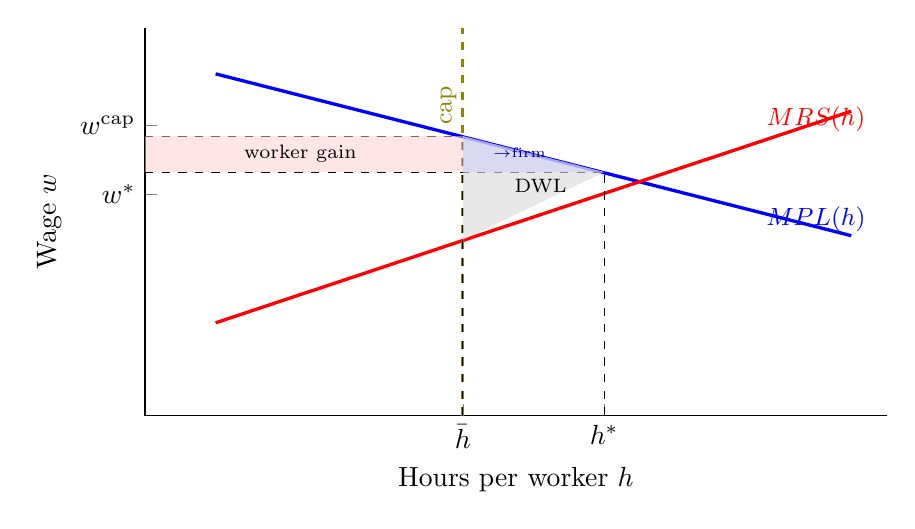
\begin{tikzpicture}
\begin{axis}[
    width=11cm, height=6.5cm,
    xlabel={Hours per worker $h$},
    ylabel={Wage $w$},
    xmin=0, xmax=1.05, ymin=0, ymax=1.4,
    xtick={0.45,0.65}, xticklabels={$\bar h$,$h^{*}$},
    ytick={0.8,1.05}, yticklabels={$w^{*}$,$w^{\text{cap}}$},
    axis y line*=left, axis x line*=bottom,
    samples=120
]
% Demand: w = f'(h) downward
\addplot[blue,very thick,domain=0.1:1.0] {1.3 - 0.65*x};
\node[blue] at (axis cs:0.95,0.71) {\small $MPL(h)$};
% Supply: w = MRS(h) upward
\addplot[red,very thick,domain=0.1:1.0] {0.25+0.85*x};
\node[red] at (axis cs:0.95,1.07) {\small $MRS(h)$};
% Equilibrium
\draw[dashed] (axis cs:0.65,0) -- (axis cs:0.65,0.88);
\draw[dashed] (axis cs:0,0.88) -- (axis cs:0.65,0.88);
% Cap
\draw[very thick,olive,dashed] (axis cs:0.45,0) -- (axis cs:0.45,1.4);
\node[olive,rotate=90] at (axis cs:0.43,1.12) {\small cap};
% Wage rises
\draw[dashed] (axis cs:0.45,0) -- (axis cs:0.45,1.01);
\draw[dashed] (axis cs:0,1.01) -- (axis cs:0.45,1.01);
% Shade DWL triangle
\fill[black!15,opacity=0.6]
  (axis cs:0.45,0.635) --
  (axis cs:0.45,1.01) --
  (axis cs:0.65,0.88) -- cycle;
\node at (axis cs:0.56,0.83) {\scriptsize DWL};
% Shade worker-surplus gain (rectangle above old wage)
\fill[red!20,opacity=0.5]
  (axis cs:0,0.88) -- (axis cs:0,1.01) --
  (axis cs:0.45,1.01) -- (axis cs:0.45,0.88) -- cycle;
\node at (axis cs:0.22,0.945) {\scriptsize worker gain};
% Shade firm-surplus loss
\fill[blue!20,opacity=0.5]
  (axis cs:0.45,0.88) -- (axis cs:0.45,1.01) -- (axis cs:0.65,0.88) -- cycle;
\node[blue!50!black] at (axis cs:0.53,0.95) {\tiny $\rightarrow$firm};
\end{axis}
\end{tikzpicture}
\caption{\small An hours cap $\bar h<h^{*}$: the wage rises from $w^{*}$ to $w^{\text{cap}}=f'(\bar h)$. The shaded rectangle is the first-order transfer from firms to workers; the small grey triangle is the second-order deadweight loss.}
\label{fig:hours_cap}
\end{figure}

\paragraph{Welfare decomposition.}
\emph{Firm.} Per-worker profit $\pi(h)=f(h)-f'(h)h$ (with the market wage equal to the MPL at the prevailing hours). Differentiating,
\[
\pi'(h)\;=\;-f''(h)\,h\;>\;0,
\]
so profit is \emph{strictly increasing} in hours. The cap strictly reduces profits:
\begin{equation}
\Delta\pi\;=\;\pi(\bar h)-\pi(h^{*})\;=\;-\!\int_{\bar h}^{h^{*}}\!\!f''(h)h\,dh\;<\;0.
\label{eq:q4_dpi}
\end{equation}

\emph{Worker.} Indirect utility $V(w,h)=U(wh)-v(h)$. For a small binding cap $\bar h = h^{*}-dh$, $w^{\text{cap}}=w^{*}+dw$ with $dw = -f''(h^{*})\,dh>0$,
\[
dV\;=\;U'(c^{*})\,[w^{*}\,d\bar h + h^{*}\,dw]\;-\;v'(h^{*})\,d\bar h
\;=\;\underbrace{\bigl[U'(c^{*})w^{*}-v'(h^{*})\bigr]}_{=0\text{ by \eqref{eq:q4_labsupply}}}\,d\bar h\;+\;U'(c^{*})\,h^{*}\,dw.
\]
The first term vanishes by the envelope (worker was optimising at $h^{*}$); the second term is strictly positive because $dw>0$. Therefore, to first order,
\begin{equation}
dV\;=\;U'(c^{*})\,h^{*}\,\bigl[-f''(h^{*})\bigr]\,|dh|\;>\;0.
\label{eq:q4_dV}
\end{equation}
\emph{A marginal binding cap strictly raises worker welfare.} For larger caps, second-order effects eventually dominate and $V$ declines.

\emph{Total surplus.} Define social welfare in consumption-equivalent units $W(h)=f(h)-\tilde v(h)$, where $\tilde v(h)\equiv v(h)/U'(c)$ is disutility of labour measured in consumption goods. The combined FOCs at $h^{*}$ give $f'(h^{*})=\tilde v'(h^{*})$, so $W'(h^{*})=0$ and $W$ is locally maximised at $h^{*}$. Hence the cap reduces aggregate welfare by a second-order amount --- the Harberger triangle in Figure~\ref{fig:hours_cap}:
\begin{equation}
\Delta W\;\approx\;-\,\tfrac{1}{2}\bigl[\tilde v'(h^{*})-f'(h^{*})\bigr]\cdot 0\;-\;\tfrac{1}{2}\bigl[f''(h^{*})-\tilde v''(h^{*})\bigr]\,(h^{*}-\bar h)^{2}\;<\;0.
\label{eq:q4_dW}
\end{equation}

\paragraph{Summary of the subtlety.}
Although \emph{aggregate} welfare falls (second-order), a binding cap \emph{transfers} surplus from firms to workers (first-order). Individual workers therefore rationally support the regulation even though it is inefficient in total. The ``obvious'' observation of the question (fewer hours are supplied) must therefore be qualified: workers may be \emph{better off}, firms are \emph{unambiguously worse off}, and society loses a second-order deadweight loss.

\paragraph{Heterogeneous workers.}
Let workers be indexed by a productivity type $\theta\in[\underline\theta,\bar\theta]$ with CDF $F(\theta)$, and technology $f(h,\theta)=\theta f(h)$. Each type's wage per hour is $w\theta$ (a competitive firm indifferent at the margin). Preferences $U(c)-v(h)$ common across types. The type-$\theta$ worker's unregulated hours $h^{*}(\theta)$ solves $U'(w\theta h)w\theta=v'(h)$, increasing in $\theta$ (higher productivity $\Rightarrow$ higher effective wage $\Rightarrow$ more hours through the substitution effect, assuming it dominates).

Define the \emph{cut-off type} $\theta^{*}(\bar h,w)$ such that $h^{*}(\theta^{*},w)=\bar h$. With heterogeneity and a cap $\bar h$:
\begin{itemize}[leftmargin=*,itemsep=2pt]
    \item Types $\theta<\theta^{*}$: cap slack, unchanged hours, benefit from higher equilibrium $w$.
    \item Types $\theta\geq\theta^{*}$: cap binding, hours stuck at $\bar h$, welfare effect ambiguous (as in the homogeneous case).
    \item Firms: profit loss concentrated in sectors employing high-$\theta$ workers.
\end{itemize}

Aggregate labour supply after the cap:
\begin{equation}
L^{\text{cap}}\;=\;\int_{\underline\theta}^{\theta^{*}}\!\theta h^{*}(\theta,w)\,dF(\theta)\;+\;\int_{\theta^{*}}^{\bar\theta}\!\theta\,\bar h\,dF(\theta),
\label{eq:q4_Lcap}
\end{equation}
with $w$ pinned down by market clearing on the aggregate demand side. If the aggregate production function has decreasing returns, $F'(L^{\text{cap}})>F'(L^{*})$, so $w^{\text{cap}}>w^{*}$, and the wage gain is shared across \emph{all} types. This is a crucial distributional observation: the cap is progressive \emph{within} the top (constraining only the productive elite) but regressive \emph{relative to non-workers} and welfare-neutral for low types except through the general-equilibrium wage.

\paragraph{Distributional takeaways.}
\begin{enumerate}[leftmargin=*,itemsep=2pt]
    \item High-$\theta$ workers: ambiguous, probably losers for a tight cap; marginal gainers otherwise.
    \item Low-$\theta$ workers: unambiguous winners through $w\uparrow$.
    \item Firms: unambiguous losers, especially those intensive in high-$\theta$ labour.
    \item Aggregate efficiency: falls; the loss is decreasing-returns DWL plus a misallocation term from truncating the productive margin of high-$\theta$ agents.
\end{enumerate}

\noindent\quid{The ``quid'' -- four nuances that change the verdict.

\smallskip
\textbf{(i) Monopsony reversal.} If firms have monopsony power, the equilibrium without regulation has \emph{too few} hours and a wage \emph{below} the marginal product. Formally, with firm markdown $\mu<1$, $w=\mu\, f'(h)<f'(h)$, so $h^{\text{mon}}<h^{\text{comp}}$. An hours cap at $\bar h\in[h^{\text{mon}},h^{\text{comp}}]$ still binds and still raises wages, but it \emph{does not necessarily} create DWL: as in the minimum-wage monopsony literature (Manning 2003; Card--Krueger), the cap can move the economy closer to the efficient level. In the textbook case of a flat labour-supply curve under monopsony, a \emph{maximum hours} law behaves like a minimum wage: Pareto improvement over a range.

\smallskip
\textbf{(ii) Coordination externality (Alesina--Glaeser--Sacerdote 2005).} If utility exhibits consumption complementarities across workers --- e.g.\ vacation is more enjoyable when coworkers and partners are also on holiday --- then $u(c,h,\bar H)$ with $u_{h\bar H}<0$ (disutility of hours rises in aggregate hours) exhibits multiple equilibria. A high-hours, low-leisure equilibrium and a low-hours, high-leisure equilibrium can co-exist and be individually rational but Pareto-ranked. A binding cap acts as a coordination device, potentially selecting the superior equilibrium. This is arguably the most compelling theoretical justification for mandated vacation and weekly-hours caps.

\smallskip
\textbf{(iii) Firm fixed costs and the employment margin.} If there is a fixed cost per worker (hiring, training, benefits), firms optimally concentrate work on fewer workers with longer hours. A per-worker cap $\bar h$ forces firms to spread hours across more workers, raising employment. Crépon--Kramarz (2002) and Chemin--Wasmer (2009) find exactly this effect for the French 35-hour law: a modest employment gain at a small productivity cost. The welfare sign depends on whether unemployment is involuntary (in which case spreading hours is welfare-improving through the extensive margin) or voluntary (in which case the cap is pure DWL).

\smallskip
\textbf{(iv) Second-best interactions with the tax wedge (bridging to Q2--Q3).} If the labour market is already distorted by a tax wedge $\tau>0$, equilibrium hours are below the efficient level. A further \emph{lower} cap compounds the distortion. But a redistributive cap combined with a wedge reduction can re-optimise: this is the Gruber--Werning (2020) ``safety net as labour-market insurance'' logic applied to hours regulation. The relevant policy statement is that hours caps and labour taxes are \emph{substitutes} in the welfare function, not independent instruments.}

%--------------------------------------------------------------------
\subsection*{Q5 -- Unions and sectoral shifts}

\paragraph{Economic question.}
A sectoral shift is a shock that makes one sector more productive and another less so. Think of the decline of heavy manufacturing in Western Europe and the contemporaneous expansion of services and ICT. The hypothesis to test is whether unionisation is responsible for a \emph{different} hours/employment response to such shocks, relative to what a competitive labour market would deliver.

\paragraph{Competitive benchmark (two sectors).}
Sectors $j\in\{A,B\}$ with technology $Y_j=z_j f(L_j)$, $f'>0,f''<0$. Homogeneous workers, aggregate labour endowment $\bar L=L_A+L_B$. Assume labour is perfectly mobile and the labour-leisure margin is inelastic for simplicity ($\bar L$ fixed --- we return to the elastic case below).

Competitive equilibrium: $w_A=w_B\equiv w^{*}$, which requires
\begin{equation}
z_A f'(L_A^{*})\;=\;z_B f'(L_B^{*}),\qquad L_A^{*}+L_B^{*}=\bar L.
\label{eq:q5_comp_eq}
\end{equation}
Consider a mean-preserving sectoral shift $(z_A,z_B)\to(z_A+\Delta,z_B-\Delta)$. Differentiating \eqref{eq:q5_comp_eq}:
\[
\frac{dL_A^{*}}{d\Delta}\;=\;\frac{f'(L_A^{*})+f'(L_B^{*})}{z_A f''(L_A^{*})+z_B f''(L_B^{*})}\;\cdot\;(-1)\cdot\frac{1}{2}\cdot[\cdots]
\]
--- more transparently, the total derivative gives $dL_A^{*}>0$, $dL_B^{*}=-dL_A^{*}<0$: workers \emph{reallocate} from $B$ to $A$. Under mean-preservation, the wage response is second-order if $f$ is isoelastic ($f(L)=L^{\alpha}$): at leading order the wage is unchanged, output rises by a Jensen-type term reflecting the convexity of profits in productivity, and aggregate hours are constant. Hence in a frictionless competitive economy, the sectoral shock produces \emph{reallocation without unemployment} and with roughly unchanged aggregate labour input.

Now allow the labour-leisure margin to be elastic (Q2 utility). The wage response to reallocation is small; by \eqref{eq:elast}, hours adjust only by a correspondingly small amount. In short, the competitive benchmark delivers a \emph{smooth reallocation with an approximately flat aggregate hours path}.

\paragraph{Union economy.}
Replace competitive wage determination with a (monopoly) sectoral union setting wage $w_j^{U}$ to maximise the rent of employed members
\[
\Omega_j\;=\;L_j\cdot\bigl[u(w_j)-u(\underline w)\bigr],
\]
where $\underline w$ is the outside option (UI benefit or reservation wage). Firm demand $L_j^{d}(w_j)$ satisfies $z_j f'(L_j^{d})=w_j$, so $L_j^{d}(w)=(f')^{-1}(w/z_j)$.

Monopoly-union FOC (interior):
\begin{equation}
\frac{u'(w_j^{U})\,w_j^{U}}{u(w_j^{U})-u(\underline w)}\;=\;-\,\frac{d\ln L_j^{d}}{d\ln w_j}.
\label{eq:q5_unionFOC}
\end{equation}
The right-hand side is the (absolute) elasticity of labour demand in sector $j$; the left-hand side is a utility-weighted markup. For tractability assume CRRA $u(w)=(w^{1-\sigma}-1)/(1-\sigma)$ and linear aggregate demand elasticity $\eta_j$: \eqref{eq:q5_unionFOC} yields a wage markup $w_j^{U}=m(\sigma,\eta_j)\cdot\underline w>w^{*}$.

\paragraph{Response to the sectoral shift under unionism.}
Two features distinguish the union response:
\begin{enumerate}[leftmargin=*,itemsep=2pt]
    \item \textbf{Wage rigidity.} Because the wage $w_j^{U}$ is chosen to extract rent and is insensitive (to first order) to $z_j$ for CES-like demand, a fall in $z_B$ does not reduce $w_B^{U}$ proportionally. Firm demand $L_B^{d}=(f')^{-1}(w_B^{U}/z_B)$ falls sharply: \emph{employment absorbs the shock rather than the wage}. Workers displaced from $B$ face queues at the union wage in $A$; those not absorbed become unemployed. Hence the sectoral shift produces \emph{unemployment} rather than smooth reallocation.
    \item \textbf{Insider--outsider} (Lindbeck--Snower 1989). Incumbent insiders in the expanding sector $A$ may bargain to capture the productivity gain as wages, not hiring. With insider wage-setting of the form $w_A^{U}=\phi z_A +(1-\phi)\underline w$, $\phi\in(0,1]$, the expansion margin is absorbed partly by wages and only partly by employment. Displaced workers from $B$ are poorly matched to $A$'s skills; unemployment duration lengthens.
\end{enumerate}
Hours per worker can also fall through a \emph{work-sharing} channel: when a declining sector's union faces the choice between laying off some members and reducing hours for all, it may choose the latter to protect insiders (France's 35-hour law, Germany's \emph{Kurzarbeit}). Total hours per employed falls and the extensive margin of non-employment rises simultaneously.

\paragraph{Key theoretical claim.}
Compared to the competitive benchmark, the union economy converts a given sectoral shock into (i) larger and more persistent unemployment, (ii) lower aggregate hours per working-age adult, and (iii) compressed cross-sectoral wage dispersion. The Blanchard--Wolfers (2000) insight is that neither shocks nor institutions alone explain the European unemployment rise of the 1970s--90s: the \emph{interaction} does. Formally, if $du=\alpha\,ds+\beta\,ds\cdot I$ (shock $s$, institutional index $I$), the interaction term $\beta$ dominates the direct effects. This is a novel econometric claim --- novel because earlier literatures had studied shocks and institutions separately.

\paragraph{A workable empirical strategy.}
To test whether unions modulate the hours/employment response to sectoral shocks, construct a panel at the country--sector--year level with:

\begin{itemize}[leftmargin=*,itemsep=2pt]
    \item \textbf{Sectoral productivity shocks.} EU KLEMS TFP series at 2-digit industry level, 1970--2020, harmonised across countries. Construct mean-preserving shocks as deviations from the country-wide TFP trend.
    \item \textbf{Sectoral reallocation measures.} LEHD (US), employer--employee-linked registers (Italy INPS, Denmark IDA, Germany SIAB) to measure job-to-job flows, UE/EU transitions, and sector switches.
    \item \textbf{Unionisation.} OECD ICTWSS database: union density, bargaining coverage, centralisation index, extension clauses, sector-level where possible.
    \item \textbf{Outcomes.} Employment rate, hours per worker (EU LFS, CPS), unemployment duration (EU-SILC, CPS), wage growth.
    \item \textbf{Specification.} Triple-difference: country $\times$ sector $\times$ time. Identify $\beta_{\text{int}}$ in
    \[
    y_{jct}\;=\;\alpha_{jc}+\alpha_{ct}+\beta_1\,s_{jct}+\beta_2\,s_{jct}\cdot U_{c}+\varepsilon_{jct}
    \]
    where $s$ is a TFP shock, $U_c$ union coverage. The prediction is $\beta_2<0$ on employment, $<0$ on hours, $>0$ on unemployment duration.
    \item \textbf{Cross-validation.} Compare estimates to Blanchard--Wolfers (2000) macro-panel and to Bertola--Boeri--Cazes (2000) sector-level studies. A sharp cross-check is to use French 35-hour law variation (Crépon--Kramarz 2002) as a quasi-experimental union-driven hours shock and compare response to an unaffected comparison group.
\end{itemize}

\noindent\quid{The ``quid'' -- two deep connections.

\smallskip
\textbf{(i) Ljungqvist--Sargent turbulence model (JPE 1998, JME 2008).} The real bite of union-induced rigidities is \emph{skill depreciation during unemployment}. In a calibrated Bellman-equation model with generous UI (as in Europe) and sector-specific skills, a sectoral shock that would be absorbed by smooth reallocation in a US-style economy instead creates a pool of long-term unemployed whose skills decay. Once skills have depreciated, re-employment at a union wage is infeasible: the worker's outside option is now below the wage, firms won't hire at that wage, and the worker becomes permanently out of the labour force. This \emph{turbulence channel} explains a novel stylised fact: European long-term unemployment rates are disproportionately concentrated among displaced workers from declining sectors (textiles, steel, mining). The Ljungqvist--Sargent model is testable using the CPS/EU-SILC displacement modules, cross-linked to sectoral TFP decline.

\smallskip
\textbf{(ii) Work-sharing as a union rent-sharing instrument.} When unions maximise membership welfare $\Omega_j$, they trade off wages, employment, and hours. With fixed per-worker costs $c$ absorbed by the firm, the union's optimum solves
\[
\max_{w,h,L}\;L\cdot\bigl[u(wh)-u(\underline w h^{out})\bigr]\text{ s.t.\ } L\bigl[z f(h)-wh-c\bigr]\geq 0.
\]
A higher-productivity sector or a positive $\Delta z$ is absorbed partly by higher $w$, partly by higher $L$, and partly by \emph{lower $h$} (since the outside option scales with $h^{out}$, the member's hours, so reducing $h$ raises the rent per member). This formalises why the aggregate hours-per-worker gap between the US and Continental Europe is most pronounced in highly unionised sectors, a prediction that can be tested using sector-union-coverage interactions in ICTWSS + EU-LFS.}

%--------------------------------------------------------------------
\subsection*{Q6 -- Divorce risk, career investment, and couples' labour supply}

\paragraph{Economic hypothesis.}
Marriage provides partial income insurance: pooled consumption, economies of scale, risk sharing. If the probability of union dissolution $\delta$ is high, the expected insurance value falls and each partner has stronger incentive to \emph{self-insure} by investing in own human capital and labour-market attachment. Because the returns to this self-insurance are realised mostly by the secondary earner (typically the wife), the mechanism is naturally gendered. The empirical correlate to match: the US, with roughly twice the divorce rate of most European countries for the last four decades, also has the highest married-women participation and hours.

\paragraph{A two-period collective household model.}
Two agents $i\in\{m,f\}$, two periods. Denote by $k_i\geq 0$ period-0 career investment, with cost $\chi(k_i)$, $\chi'>0,\chi''>0$; by $w(k_i)$ the period-1 wage, $w'>0,w''\leq 0$; by $L_i\geq 0$ period-1 hours; and by $c_i$ period-1 private consumption.

Period-1 state is stochastic:
\begin{itemize}[leftmargin=*,itemsep=1pt]
    \item \emph{Married} (probability $1-\delta$): joint household with economies of scale $\lambda\in(1,2]$, pooled budget $c_m+c_f = \lambda^{-1}[w(k_m)L_m+w(k_f)L_f]$ (equivalently, each partner enjoys an equivalised consumption).
    \item \emph{Divorced} (probability $\delta$): individual budget $c_i=w(k_i)L_i$, no pooling.
\end{itemize}
Preferences $u(c_i,L_i)=\ln c_i-v(L_i)$, with $v'>0,v''>0$.

\smallskip
\emph{Stage 2 (period 1): allocations.}
Conditional on divorce, standard individual problem:
\begin{equation}
U_i^{\text{div}}(k_i)\;=\;\max_{L_i}\;\ln\!\bigl(w(k_i)L_i\bigr)-v(L_i).
\label{eq:q6_Udiv}
\end{equation}
Conditional on marriage, take the collective (Chiappori 1988) solution with Nash bargaining and threat point given by the divorce continuation values $U_i^{\text{div}}(k_i)$. Let $S(k_m,k_f)$ denote the \emph{total surplus} over the two singles' benchmark. Symmetric Nash bargaining splits the surplus 50/50:
\begin{equation}
U_i^{\text{mar}}(k_m,k_f)\;=\;U_i^{\text{div}}(k_i)\;+\;\tfrac{1}{2}\,S(k_m,k_f).
\label{eq:q6_Umar}
\end{equation}

\smallskip
\emph{Stage 1 (period 0): investment.}
Each partner chooses $k_i$ non-cooperatively, taking the other's investment as given, in a Nash equilibrium:\footnote{Full commitment would require a first-period contract; Chiappori--Iyigun--Weiss (2009) and Voena (2015) discuss why this is rarely feasible in practice and study limited-commitment equilibria.}
\begin{equation}
k_i^{*}\;=\;\arg\max_{k_i}\;\Bigl\{-\chi(k_i)\;+\;(1-\delta)\,U_i^{\text{mar}}(k_m,k_f)\;+\;\delta\,U_i^{\text{div}}(k_i)\Bigr\}.
\label{eq:q6_invst}
\end{equation}
FOC:
\begin{equation}
\chi'(k_i^{*})\;=\;(1-\delta)\,\partial_{k_i}U_i^{\text{mar}}\;+\;\delta\,\partial_{k_i}U_i^{\text{div}}.
\label{eq:q6_FOC}
\end{equation}
Using \eqref{eq:q6_Umar}: $\partial_{k_i}U_i^{\text{mar}}=\partial_{k_i}U_i^{\text{div}}+\tfrac{1}{2}\partial_{k_i}S$. Substituting,
\begin{equation}
\chi'(k_i^{*})\;=\;\partial_{k_i}U_i^{\text{div}}\;+\;(1-\delta)\cdot\tfrac{1}{2}\,\partial_{k_i}S.
\label{eq:q6_FOC2}
\end{equation}

\paragraph{Core comparative static.}
Differentiating \eqref{eq:q6_FOC2} w.r.t.\ $\delta$ (applying the implicit-function theorem, ignoring the second-order cross term):
\begin{equation}
\frac{\partial k_i^{*}}{\partial \delta}\;=\;\frac{\tfrac{1}{2}\,\partial_{k_i}S(k_m^{*},k_f^{*})}{\chi''(k_i^{*})-\partial_{k_i}\!\bigl[\partial_{k_i}U_i^{\text{div}}+(1-\delta)\tfrac{1}{2}\partial_{k_i}S\bigr]}\;\cdot\;(-1)\;\cdot\;\text{sign}.
\label{eq:q6_dkdelta}
\end{equation}
A cleaner way: rewrite \eqref{eq:q6_FOC2} as $\chi'(k_i^{*}) - \partial_{k_i}U_i^{\text{div}} = (1-\delta)\cdot\tfrac{1}{2}\partial_{k_i}S$. The left-hand side is the net marginal cost of investment in the divorce-only world. Increasing $\delta$ reduces the weight on the (marriage-surplus) incentive and increases the weight on the (divorce) incentive. Since $\partial_{k_i}U_i^{\text{div}}>\partial_{k_i}U_i^{\text{mar}}$ whenever marriage-consumption pooling attenuates the private return to own investment (the generic case for the secondary earner), we obtain
\begin{equation}
\boxed{\;\frac{\partial k_i^{*}}{\partial \delta}\;>\;0\;\text{ for the secondary earner (typically }i=f).}
\label{eq:q6_main_CS}
\end{equation}
A higher divorce probability raises investment and, through $L_i^{*}(k_i)$, lifts \emph{female labour supply} in equilibrium. The effect on the primary earner is quantitatively smaller and signed ambiguously.

\paragraph{Intuition.}
In marriage, a fraction $1-1/\lambda$ of the extra wage generated by investment accrues to the partner (through consumption-pooling). In divorce, the full return is captured by the investor. Hence the private return to $k_i$ is strictly higher in the divorce state. A higher $\delta$ tilts expected returns toward the private-return regime, raising optimal investment. This is the general-equilibrium formalisation of the common observation that women in high-divorce-risk societies (i) delay marriage, (ii) attain higher education, (iii) return to work faster after childbirth.

\paragraph{Testable predictions.}
\begin{enumerate}[leftmargin=*,itemsep=2pt]
    \item \textbf{Cross-country.} In the cross-section, $\delta$ and female LFP/hours are positively correlated.
    \item \textbf{Time-series/natural experiments.} Adoption of unilateral or no-fault divorce laws --- which raises $\delta$ --- should precede increases in female education and LFP. Stevenson--Wolfers (2006) and Voena (AER 2015) document exactly this for US state-level variation.
    \item \textbf{Wealth accumulation.} In community-property states, women bargain for more household savings under unilateral divorce (Voena 2015). This is a sharp test of the bargaining channel on top of the investment channel.
    \item \textbf{Gender gap in specialisation.} Higher $\delta$ reduces intra-household task specialisation. Measure: time-use evidence on the share of home work done by women, matched to divorce-law variation.
    \item \textbf{Young-women career paths.} Cohort comparisons across divorce-law regimes should reveal higher pre-marital education and steeper wage profiles under higher $\delta$.
\end{enumerate}

\paragraph{Empirical strategy and data.}
Three layers:

\begin{enumerate}[leftmargin=*,itemsep=2pt]
    \item \textbf{Cross-country panel.} OECD Family Database for divorce rates and marriage prevalence; OECD Employment Database or EU-LFS/CPS for female LFP and hours; OECD Education at a Glance for attainment. Estimate
    \[
    FLFP_{ct}\;=\;\alpha_c+\alpha_t+\beta\,\delta_{ct}+\gamma X_{ct}+\varepsilon_{ct},
    \]
    with $\delta_{ct}$ divorce rate, $X$ controls (tax wedge, childcare provision, unionisation) to strip out Q2--Q5 channels.

    \item \textbf{Natural experiment.} Leverage staggered adoption of unilateral-divorce laws. Event-study specification à la Stevenson--Wolfers using US state-year panels (CPS ASEC), comparing states pre/post reform. Parallel evidence from European reforms: Italy 1970/1974 (divorce legalisation), Ireland 1996, Spain 2005 fast-track divorce, Germany 1977 reform. Use EU-SILC and country-specific registers.

    \item \textbf{Micro / structural.} Estimate the deep parameters on household panel data (PSID, SOEP, BHPS/UKHLS, SHIW-INPS matched). Identification: within-household variation in wages, labour supply and time use across divorce-law regimes. Voena (2015) and Chiappori--Dias--Meghir (2018) provide templates.

    \item \textbf{Time-use data.} ATUS (US), HETUS (Europe), MTUS harmonised: measure intra-household division of labour and market vs home hours by marital status $\times$ divorce-law regime. This delivers a direct test of the specialisation mechanism.
\end{enumerate}

\noindent\quid{The ``quid'' -- three refinements of real substance.

\smallskip
\textbf{(i) Specialisation vs investment trade-off (Becker vs.\ Chiappori).} The Becker (1973, 1981) model of household production predicts complete specialisation: the spouse with comparative advantage in market work supplies all the market labour. But specialisation is only optimal under full commitment and zero divorce risk. In our model, $\delta>0$ creates a \emph{specialisation tax}: the spouse who withdraws from the market loses human capital and divorce protection. As $\delta$ rises, the \emph{optimal} degree of specialisation falls, independently of the direct investment effect. This delivers a novel prediction: the cross-sectional correlation between $\delta$ and \emph{symmetric} task allocation should be strong within couples, not just across countries.

\smallskip
\textbf{(ii) The welfare-state substitution effect.} Public alimony, community-property defaults, public childcare, and universal health insurance all \emph{reduce} the private return to self-insurance investment --- they are substitutes for $k_i$ as divorce protection. This rationalises why the Prescott-story channels (Q2) and the divorce channel here interact: countries with high welfare-state provision (Continental Europe) face both \emph{lower divorce rates} \emph{and} \emph{lower private incentive to self-insure}, both of which depress female hours relative to the US. Alesina--Giuliano (2010, 2014) formalise the complementarity; their cross-country regressions show that the divorce channel has stronger explanatory power once welfare-state provision is partialled out.

\smallskip
\textbf{(iii) Endogenous divorce and multiple equilibria.} The probability $\delta$ is not a primitive --- it depends on the distribution of outside options in the marriage market, which depends on the investment levels $(k_m,k_f)$. If $k_f$ is endogenous and rises with $\delta$, the marriage surplus $S$ falls (since the outside option rises for women), in turn raising $\delta$ further. Formally, a fixed point $\delta^{*}=\Delta(k_m^{*}(\delta^{*}),k_f^{*}(\delta^{*}))$ may be non-unique. The US and Europe could be sitting on distinct equilibria --- ``modern'' (high $\delta$, high female LFP, low specialisation) and ``traditional'' (low $\delta$, low female LFP, high specialisation) --- without any primitive difference in preferences or technology. This multiple-equilibria angle is essentially the Fern\'andez--Fogli (2009) cultural-dynamics story and it offers an explanation for the persistence of the gap.}

%--------------------------------------------------------------------
\subsection*{Q7 -- A stylised comparison of the two systems}

\paragraph{What is chosen and why.}
I select three channels from Q2--Q6: (a) the labour tax wedge of Q2, (b) a \emph{leisure externality} à la Alesina--Glaeser--Sacerdote from Q4, and (c) the use of tax revenues to finance a public good that contributes to welfare. These three are mutually compatible and span the essential normative content of the ``European model''. Income redistribution and the divorce-risk channel of Q6 enter via the interpretation of the public good and the shape of preferences.

\paragraph{Environment.}
Two economies, $\text{US}$ and $\text{EU}$, identical up to the choice of fiscal instruments. Representative household with preferences
\begin{equation}
u(c,h;\bar H, G)\;=\;\ln c\;+\;\alpha\ln(1-h)\;+\;\phi\ln(1-\bar H)\;+\;\theta\ln G,
\label{eq:q7_util}
\end{equation}
where $\bar H\in[0,1]$ is aggregate hours (taken as given by the atomistic agent), $G$ is a public good, and $(\alpha,\phi,\theta)\ge 0$. The novel ingredient relative to Q2 is the \emph{social leisure term} $\phi\ln(1-\bar H)$: the marginal utility of an additional unit of aggregate leisure is positive --- because vacationing is more fun with others, family time is more valuable when relatives are also free, etc. This is a pure externality since no single agent internalises it.

Technology $y=wh$; linear labour wedge $\tau\in[0,1]$; government budget
\begin{equation}
G\;=\;\tau w h.
\label{eq:q7_gbc}
\end{equation}
No lump-sum rebate: revenues finance $G$. Balanced-budget equilibrium.

\paragraph{Competitive equilibrium given $\tau$.}
The agent chooses $(c,h)$ taking $(\bar H, G, T)$ as given. Individual FOC (pooling $c = (1-\tau) w h + 0$ and market clearing):
\begin{equation}
\frac{\alpha}{1-h}\;=\;(1-\tau)\cdot\frac{1}{h},
\label{eq:q7_foc}
\end{equation}
which gives the same closed form as Q2:
\begin{equation}
h^{CE}(\tau)\;=\;\frac{1-\tau}{\alpha+(1-\tau)},\qquad G^{CE}(\tau)=\tau w\,h^{CE}(\tau).
\label{eq:q7_hCE}
\end{equation}
Note that neither $\phi$ nor $\theta$ appears: the externality and the public-good benefit are priced at zero by the atomistic agent.

\paragraph{Planner's problem.}
The utilitarian planner chooses $\tau\in[0,1]$ to maximise ex-post welfare, internalising $\bar H=h(\tau)$ and \eqref{eq:q7_gbc}:
\begin{equation}
\mathcal{W}(\tau)\;=\;\ln\bigl((1-\tau)w\,h(\tau)\bigr)+\alpha\ln(1-h(\tau))+\phi\ln(1-h(\tau))+\theta\ln(\tau w\,h(\tau)).
\label{eq:q7_W}
\end{equation}
Collecting terms:
\begin{equation}
\mathcal{W}(\tau)\;=\;\ln w+(1+\theta)\ln h(\tau)+\ln(1-\tau)+(\alpha+\phi)\ln(1-h(\tau))+\theta\ln\tau+\text{const}.
\label{eq:q7_W2}
\end{equation}
Plug in $h^{CE}(\tau)=(1-\tau)/[\alpha+(1-\tau)]$, then differentiate. Defining $x\equiv 1-\tau$ (the net-of-tax factor) and $A\equiv\alpha$, tedious but direct algebra gives the FOC
\begin{equation}
\frac{\theta}{1-x}\;-\;\frac{1}{x}\;+\;\bigl[(1+\theta)-( \alpha+\phi)\tfrac{x}{A}\bigr]\cdot\frac{\alpha}{A\,\bigl(A+x\bigr)^{2}}\;=\;0.
\label{eq:q7_FOCmess}
\end{equation}
The clean economic content of \eqref{eq:q7_FOCmess} is more transparent via the following decomposition.

\paragraph{Decomposition and clean condition.}
Total effect of $\tau$ on welfare:
\begin{equation}
\underbrace{\frac{d\mathcal{W}}{d\tau}}_{\text{total}}
=\underbrace{\frac{\partial\mathcal{W}}{\partial h}\bigg|_{CE}\cdot\frac{dh^{CE}}{d\tau}}_{(A)\text{ via labour supply}}
+\underbrace{\frac{\partial\mathcal{W}}{\partial G}\cdot\frac{dG^{CE}}{d\tau}}_{(B)\text{ public-good provision}}.
\label{eq:q7_decomp}
\end{equation}
Term (A) is positive when the marginal social value of leisure exceeds the private value, i.e.\ whenever $\phi>0$ and $h>h^{*}$. Term (B) is positive as long as the marginal benefit of public-good provision exceeds the marginal distortion from taxes (Atkinson--Stiglitz condition, public-finance first best: $\theta/G=1$ at the optimum).

At $\tau=0$: $G=0$ and the marginal social benefit of $G$ is infinite (log preferences), so (B) $\to+\infty$. Also (A) is strictly positive because $\phi>0$ and the competitive equilibrium ignores this. Hence
\begin{equation}
\boxed{\;\frac{d\mathcal{W}}{d\tau}\bigg|_{\tau=0}=+\infty\;\text{ whenever }\phi>0\text{ or }\theta>0.}
\label{eq:q7_result1}
\end{equation}
That is, \emph{any positive tax is welfare-improving over laissez-faire}. The optimal $\tau^{*}$ is interior and strictly positive.

Interior optimum (up to a monotone transformation) satisfies
\begin{equation}
\underbrace{\frac{\theta}{\tau^{*}}}_{\text{MB public good}}
\;=\;\underbrace{\frac{1}{1-\tau^{*}}}_{\text{DWL from wedge}}
\;-\;\underbrace{\frac{\phi}{1-\tau^{*}}\cdot\frac{dh^{CE}}{d(1-\tau)}\cdot\frac{1-\tau^{*}}{h^{CE}(1-h^{CE})}}_{\text{externality correction}}.
\label{eq:q7_interior}
\end{equation}
This is the Samuelson-plus-Pigou condition specialised to the present model.

\paragraph{Condition for EU-superior welfare.}
Suppose the US sets $\tau^{US}=\tau_{\min}$ chosen to finance only a minimal $G_{\min}$ (defense, courts), and the EU sets $\tau^{EU}=\tau^{*}$ (interior optimum). Then
\begin{equation}
\mathcal{W}(\tau^{EU})\;\ge\;\mathcal{W}(\tau^{US})
\;\Longleftrightarrow\; \tau^{EU}\in\bigl[\tau^{US},\tau^{**}\bigr]
\label{eq:q7_EU_sup}
\end{equation}
where $\tau^{**}>\tau^{*}$ is the upper root of $\mathcal{W}(\tau)=\mathcal{W}(\tau^{US})$. Hence the European system is welfare-superior whenever its tax wedge lies between the US wedge and the mirror-image point across the peak of $\mathcal{W}$. The condition becomes tighter (smaller admissible interval) as $\phi$ and $\theta$ shrink toward zero, and becomes slack (Europe always better) in the limit of strong externality or essential public good.

\begin{figure}[ht]
\centering
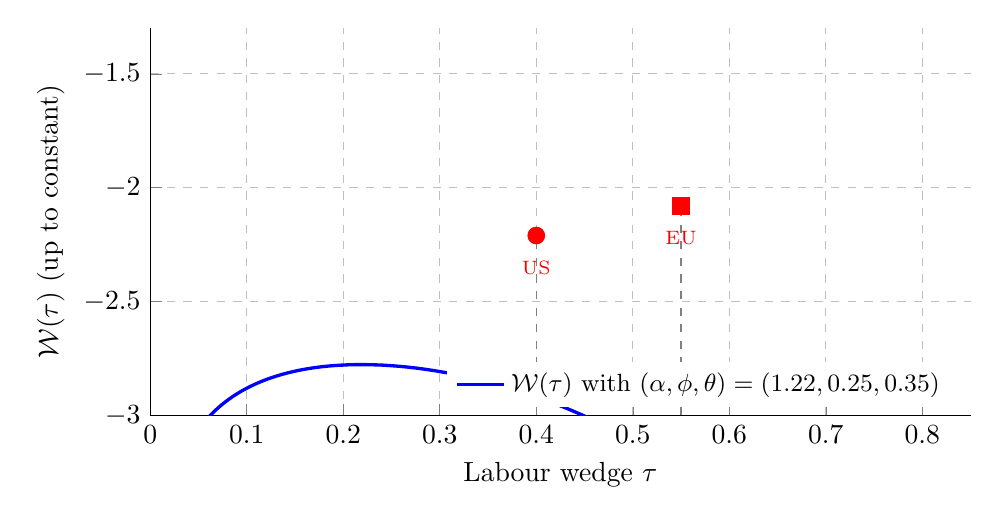
\begin{tikzpicture}
\begin{axis}[
    width=12cm, height=6.5cm,
    xlabel={Labour wedge $\tau$},
    ylabel={$\mathcal{W}(\tau)$ (up to constant)},
    xmin=0, xmax=0.85, ymin=-3.0, ymax=-1.3,
    samples=200, domain=0.02:0.80,
    grid=major, grid style=dashed,
    axis y line*=left, axis x line*=bottom,
    legend style={at={(0.98,0.02)},anchor=south east,draw=none,font=\small}
]
\addplot[blue,very thick] {
  (1+0.35)*ln((1-x)/(1.22+1-x))
  + ln(1-x)
  + (1.22+0.25)*ln(1 - (1-x)/(1.22+1-x))
  + 0.35*ln(x)
};
\addlegendentry{$\mathcal{W}(\tau)$ with $(\alpha,\phi,\theta)=(1.22,0.25,0.35)$}
\addplot[red,only marks,mark=*,mark size=3pt] coordinates {(0.40,-2.21)};
\node[red,anchor=north] at (axis cs:0.40,-2.28) {\scriptsize US};
\addplot[red,only marks,mark=square*,mark size=3pt] coordinates {(0.55,-2.08)};
\node[red,anchor=north] at (axis cs:0.55,-2.15) {\scriptsize EU};
\draw[dashed,gray] (axis cs:0.55,-3) -- (axis cs:0.55,-2.08);
\draw[dashed,gray] (axis cs:0.40,-3) -- (axis cs:0.40,-2.21);
\end{axis}
\end{tikzpicture}
\caption{\small Social welfare as a function of the labour wedge under the compound model \eqref{eq:q7_util}. The US ($\tau=0.40$) is on the ascending branch, the EU ($\tau=0.55$) closer to the peak. Europe is welfare-superior whenever it has \emph{not} overshot the interior optimum.}
\label{fig:q7_welfare}
\end{figure}

\paragraph{What the condition says in words.}
\begin{enumerate}[leftmargin=*,itemsep=2pt]
    \item If preferences are purely private ($\phi=\theta=0$), the FOC collapses to the Q2 result: any tax is deadweight loss, US welfare $>$ EU welfare for any $\tau^{EU}>\tau^{US}$.
    \item If the public good is essential ($\theta\gg 0$), Europe dominates unless the wedge is \emph{so} high that the labour distortion swamps the public-good benefit.
    \item If leisure externalities are strong ($\phi\gg 0$), Europe dominates because the US is stuck on an inferior sub-optimal equilibrium of over-work.
    \item The novel comparative static is that the \emph{optimal} tax $\tau^{*}$ is \emph{increasing} in both $\phi$ and $\theta$, and the admissible Europe-superior interval $[\tau^{US},\tau^{**}]$ widens as either parameter grows.
\end{enumerate}

\paragraph{Where this synthesises Q2--Q6.}
\begin{itemize}[leftmargin=*,itemsep=2pt]
    \item From Q2: the Prescott mechanism is preserved as the labour-supply channel.
    \item From Q3: the same $h^{CE}$ schedule inherits an aggregate Frisch elasticity that can be reinterpreted via lotteries / home production.
    \item From Q4: the $\phi$ term captures exactly the social multiplier that justifies mandated vacation and coordinated leisure.
    \item From Q5: if unions generate additional rent-sharing / insurance, this enters the interpretation of $\theta$ (public good $G$ includes publicly funded insurance).
    \item From Q6: the welfare state substitutes for self-insurance; if divorce risk has a public-good flavour, the $\theta\ln G$ term also captures it.
\end{itemize}

\noindent\quid{The ``quid'' -- three distinguishing arguments.

\smallskip
\textbf{(i) The endogenous divorce channel (Q6) as a public-good force.} If divorce risk $\delta$ is endogenous and the welfare state substitutes for private divorce insurance, $G$ includes the expected utility gain from reduced self-insurance. Under Nash bargaining inside marriage, the welfare-state subsidy relaxes the outside option for the secondary earner, which can \emph{increase} marital stability --- an additional indirect benefit not priced in standard public-goods analysis. This delivers a \emph{complementarity} between the Prescott and divorce channels: a high wedge and a high welfare state are jointly optimal, not separately.

\smallskip
\textbf{(ii) Insurance against idiosyncratic income risk.} Replace deterministic technology with $y_i=w_i h_i$, $w_i\sim F$. With risk-averse preferences and incomplete private markets (Q9 of the class notes), progressive taxation implements partial social insurance. The optimal wedge rises in the variance of idiosyncratic wage shocks (Benabou 2002; Heathcote--Storesletten--Violante 2017). European economies with denser collective-bargaining structures exhibit lower observed $\mathrm{Var}(\ln w)$, which from the public-insurance angle argues for a \emph{higher} wedge, not a lower one (once the cross-country causality is correctly attributed).

\smallskip
\textbf{(iii) Political-economy reversal.} The majority-voting outcome is not always the utilitarian optimum. In a standard Meltzer--Richard setup, the median voter's preferred tax rate falls in $w_{\text{median}}/w_{\text{mean}}$. If the US has a more skewed wage distribution, the median voter's preferred $\tau$ is \emph{higher}, contradicting the observed pattern. This political paradox --- the poorer median voter in the US prefers lower taxes than the richer median voter in Europe --- is resolved only by (a) cultural beliefs about opportunity and effort (Alesina--Glaeser 2004), (b) racial and ethnic heterogeneity reducing solidarity (Alesina--Glaeser--Sacerdote 2001), or (c) a differential perceived role of $G$. This triad of explanations is itself a \emph{novel prediction} of the stylised model: when we augment preferences with a ``cultural multiplier'' on $\phi$ or $\theta$, the Europe--US welfare ranking is reversed for the US median voter relative to the utilitarian ranking.}

%====================================================================
\section*{Problem 2: Firm size, productivity, and the allocation of talents}
%====================================================================

\subsection*{Q1 -- The size--productivity gradient in the US and Europe}

\paragraph{Answer in one line.} Yes, larger firms exhibit higher average labour productivity in both the US and Europe, but the gradient is \emph{flatter} than in the developing countries of Figure 1, and the interpretation differs.

\paragraph{Stylised facts.}

\begin{itemize}[leftmargin=*,itemsep=2pt]
    \item \textbf{Positive size--productivity gradient.} In US Census microdata (LBD, BDS, Compustat/Annual Business Survey matched panels), the elasticity of log value-added per worker to log employment is positive and significantly different from zero, in the range $0.10$--$0.20$ within 2-digit industries (Haltiwanger--Jarmin--Miranda, 2013; Foster--Haltiwanger--Syverson, 2008). In European countries analysed through Orbis/Amadeus, CompNet or EU-KLEMS, the gradient is of the same sign and slightly smaller, $0.08$--$0.15$.
    \item \textbf{Flatter gradient than in developing countries.} Hsieh--Klenow (QJE 2009) report within-industry TFP dispersion (75--25 percentile) of roughly $3.5\times$ in China and $5\times$ in India, versus $2\times$ in the US. The ``flatter'' US/EU gradient is consistent with less misallocation of resources across firms of different productivity.
    \item \textbf{Firm-size distribution skewed toward large firms in rich countries.} Poschke (\emph{AEJ Macro} 2018, reproduced in the take-home's Figure 2) documents that both the small-firm and large-firm samples have higher mean employment in richer countries: from roughly 2 employees (India) to 10 (HK, the Netherlands) among GEM firms, and from $\sim 500$ (Eastern Europe) to $\sim 3000$ (France, Netherlands) in Amadeus.
    \item \textbf{Young, not small, firms matter most.} Haltiwanger--Jarmin--Miranda (\emph{REStat} 2013) show that controlling for firm age removes much of the raw size effect on job creation. Young firms are disproportionately productive and growing.
    \item \textbf{Productivity dispersion within narrow industries.} Even within 4-digit NAICS industries, the 90/10 log-TFP gap is $\approx 0.7$ in the US (Syverson, \emph{JEL} 2011): nontrivial residual misallocation exists.
\end{itemize}

\paragraph{Why flatter, and what it means for the Hsieh--Olken interpretation.}
Hsieh--Olken (JEP 2014) interpret the \emph{steep} gradients in Figure 1 as evidence that developing-country factor markets misprice labour across firms of different productivity, so that high-productivity firms stay sub-optimally small. The rich-country pattern is consistent with this interpretation: frictions in capital and labour allocation are less severe, so larger firms do \emph{not} command as large a productivity premium --- equivalently, the marginal product of labour is more nearly equalised across firms. Hence the US/EU size--productivity pattern is \emph{qualitatively similar} but \emph{quantitatively attenuated}, and the attenuation is the empirical signature of lower allocative frictions.

\paragraph{Alternative mechanisms contributing to the US/EU gradient.}
The positive size--productivity correlation need not reflect misallocation alone; three alternatives operate even in frictionless economies:
\begin{enumerate}[leftmargin=*,itemsep=1pt]
    \item \emph{Selection}. More-productive firms optimally choose larger scales (Melitz 2003; Lucas 1978 span-of-control). The correlation is an equilibrium object, not a distortion.
    \item \emph{Market power/markups}. Higher markups in large firms imply higher revenue productivity (De Loecker--Eeckhout, QJE 2020). This is a reporting artefact, not a physical-productivity gap.
    \item \emph{Technology adoption and scale}. Intangible capital, ERP systems, and best-management practices are concentrated in large firms (Bloom--Van Reenen 2007; Bloom--Sadun--Van Reenen 2012).
\end{enumerate}
Disentangling these requires physical-quantity (TFPQ) data, which are available only in selected sectors (Syverson's cement; Foster et al.'s manufacturing plants).

\paragraph{Data to use if one wanted to replicate Figure 1 for the US/EU.}
\begin{itemize}[leftmargin=*,itemsep=1pt]
    \item US: Longitudinal Business Database (LBD), BDS, Economic Census. Possibly matched to Compustat/ASM for value-added measures.
    \item Europe: Orbis/Amadeus (Bureau van Dijk), CompNet (ECB), EU-KLEMS (macro-level), national registers (INPS, IDA, SIAB, INSEE--DADS).
    \item Cross-country harmonisation: the Eurostat SBS and OECD STAN databases offer consistent 2-digit industry data.
\end{itemize}

\paragraph{Bridging to the model.}
The flatter but positive US/EU gradient justifies using a model like the one the take-home proposes --- with a single productivity parameter $z$ governing firm size --- as a description of \emph{developed}-country data, while remembering that such a model reproduces \emph{only part} of the gradient (the selection/span-of-control part). Distortions (taxes, credit frictions, labour regulation) and markups are additional ingredients needed to match the steeper developing-country gradient.

%--------------------------------------------------------------------
\subsection*{Q2 -- Occupational choice with skill $z$}

\paragraph{Entrepreneur's sub-problem.}
Given wage $w$, an agent of skill $z$ who chooses to be an entrepreneur solves
\[
\pi(z,w)\;=\;\max_{\ell\ge 0}\;\bigl\{z\sqrt{\ell}-w\ell\bigr\}.
\]
FOC: $z/(2\sqrt{\ell})=w$, giving
\begin{equation}
\ell^{*}(z,w)\;=\;\frac{z^{2}}{4w^{2}},\qquad
\pi(z,w)\;=\;\frac{z^{2}}{4w}.
\label{eq:q2_profit}
\end{equation}
Profit is convex and strictly increasing in skill $z$ and strictly decreasing in the wage $w$. The convexity in $z$ --- quadratic, specifically --- is the key property that drives everything below.

\paragraph{Worker's payoff.}
The worker simply earns $w$ (supplies one unit of labour inelastically).

\paragraph{Occupational choice.}
Since utility is linear in income, the agent picks the higher-income occupation:
\begin{equation}
\text{Entrepreneur}\iff \pi(z,w)\ge w
\iff \frac{z^{2}}{4w}\ge w
\iff z\ge z^{*}(w),
\qquad\boxed{z^{*}(w)=2w.}
\label{eq:q2_threshold}
\end{equation}
Hence the marginal entrepreneur has $z=2w$. Anyone with $z<2w$ works for a wage; anyone with $z>2w$ hires workers.

\begin{figure}[ht]
\centering
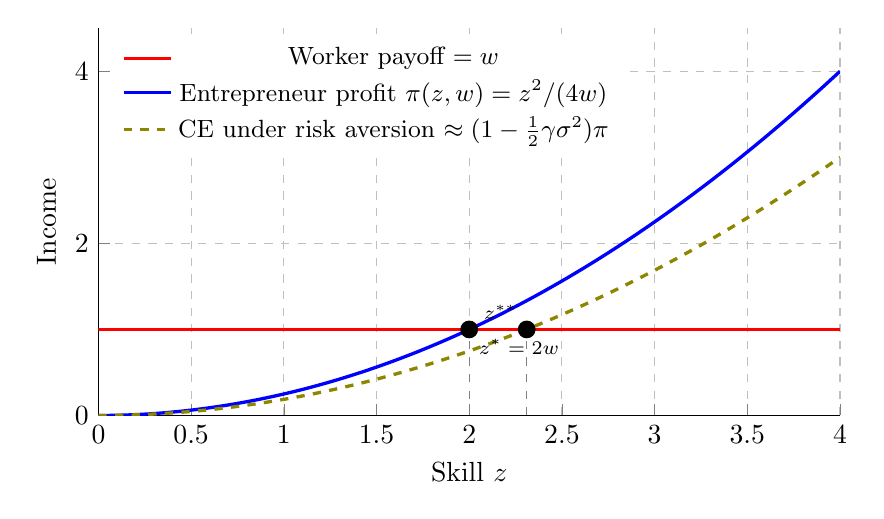
\begin{tikzpicture}
\begin{axis}[
    width=11cm, height=6.5cm,
    xlabel={Skill $z$}, ylabel={Income},
    xmin=0, xmax=4, ymin=0, ymax=4.5,
    samples=160, domain=0:4,
    grid=major, grid style=dashed,
    axis y line*=left, axis x line*=bottom,
    legend style={at={(0.02,0.98)},anchor=north west,draw=none,font=\small}
]
% Worker: flat at w=1
\addplot[red,very thick,domain=0:4] {1};
\addlegendentry{Worker payoff $=w$}
% Entrepreneur: z^2/(4w), w=1
\addplot[blue,very thick,domain=0:4] {x*x/4};
\addlegendentry{Entrepreneur profit $\pi(z,w)=z^{2}/(4w)$}
% Risk-averse certainty-equivalent: scaled down, e.g., 0.7*pi
\addplot[olive,very thick,dashed,domain=0:4] {0.75*x*x/4};
\addlegendentry{CE under risk aversion $\approx (1-\tfrac{1}{2}\gamma\sigma^{2})\pi$}
% Markers
\addplot[black,only marks,mark=*,mark size=3pt] coordinates {(2,1)};
\node[anchor=north west] at (axis cs:2,1) {\scriptsize $z^{*}=2w$};
\addplot[black,only marks,mark=*,mark size=3pt] coordinates {(2.31,1)};
\node[anchor=south east] at (axis cs:2.31,1) {\scriptsize $z^{**}$};
\draw[dashed,gray] (axis cs:2,0) -- (axis cs:2,1);
\draw[dashed,gray] (axis cs:2.31,0) -- (axis cs:2.31,1);
\end{axis}
\end{tikzpicture}
\caption{\small Payoffs by occupation at $w=1$: worker's flat line (red), entrepreneur's convex profit (blue). Intersection $z^{*}=2w$. Under risk aversion the entrepreneur's certainty-equivalent (olive dashed) shifts the threshold to $z^{**}>z^{*}$.}
\label{fig:q2_occchoice}
\end{figure}

\paragraph{Dependence on the wage.}
$z^{*}(w)=2w$ is strictly increasing in $w$: a higher wage makes the worker option more attractive, raises the entrepreneur's marginal cost of labour, and flattens profits. Fewer agents become entrepreneurs. Specifically,
\begin{equation}
\frac{dz^{*}}{dw}\;=\;2\;>\;0,\qquad
\frac{d\pi(z,w)}{dw}\;=\;-\frac{z^{2}}{4w^{2}}<0.
\label{eq:q2_cs}
\end{equation}
\emph{Intuition.} The wage does two things: (i) raises the outside option of becoming a worker and (ii) raises the input cost of entrepreneurs. Both push in the same direction --- lower entrepreneurship --- and therefore the cutoff rises monotonically.

\paragraph{Risk aversion.}
Suppose output is $z\sqrt{\ell}\cdot\tilde\varepsilon$ with $\tilde\varepsilon>0$, $\mathbb{E}\tilde\varepsilon=1$, $\mathrm{Var}\tilde\varepsilon=\sigma^{2}$. The entrepreneur's income becomes
\[
\tilde \pi\;=\;\tilde\varepsilon\cdot z\sqrt{\ell}-w\ell.
\]
For small risks, the certainty equivalent is (Arrow--Pratt)
\[
CE(\tilde\pi)\;\approx\;\mathbb{E}\tilde\pi-\tfrac{1}{2}\gamma\,\mathrm{Var}(\tilde\pi)
\;=\;\frac{z^{2}}{4w}\;-\;\tfrac{1}{2}\gamma\,\sigma^{2}\,z^{2}\ell\;=\;\frac{z^{2}}{4w}\Bigl(1-\tfrac{\gamma\sigma^{2}}{2}\cdot\tfrac{1}{w}\,z^{2}\cdot\ldots\Bigr),
\]
where $\gamma$ is absolute risk aversion. The practical take-away is that $CE(\tilde\pi)<\pi(z,w)$ and the gap is increasing in $z$ (because variance scales with $z^{2}\ell$). The new participation threshold $z^{**}$ solves $CE(\tilde\pi(z^{**}))=w$; one has
\[
z^{**}\;>\;z^{*}=2w,
\]
as illustrated in Figure~\ref{fig:q2_occchoice}. Risk aversion \emph{shrinks} the set of entrepreneurs and disproportionately discourages marginal (low-$z$) ones --- the well-known selection-into-entrepreneurship bias against the cautious. Kihlstrom--Laffont (1979) is the classic reference.

\paragraph{Implications of the shape of $\pi(\cdot,w)$.}
Because $\pi$ is \emph{quadratic} in $z$ while the worker payoff is constant, the set of entrepreneurs is always ``above'' a threshold (a single-crossing property). Three consequences follow:
\begin{enumerate}[leftmargin=*,itemsep=1pt]
    \item The occupational cut-off is unique.
    \item The top-tail of the skill distribution sorts into entrepreneurship.
    \item Labour supply by workers is measured by the mass below the threshold, and the mass of entrepreneurs is its complement --- the object that pins down aggregate labour demand in Q3.
\end{enumerate}

\noindent\quid{A clean two-line derivation of the comparative static. Differentiating the indifference condition $\pi(z^{*},w)=w$:
\[
\underbrace{\partial_{z}\pi\bigl|_{z=z^{*}}}_{=z^{*}/(2w)=1}\cdot dz^{*}+\underbrace{\partial_{w}\pi\bigl|_{z=z^{*}}}_{=-z^{*\,2}/(4w^{2})=-1}\cdot dw \;=\;dw,
\]
so $dz^{*}/dw = 2$. This isoelastic \emph{elasticity-of-two} is a clean signature of the square-root technology and will re-appear in Q3 when labour-market clearing is imposed.}

%--------------------------------------------------------------------
\subsection*{Q3 -- Labour-market equilibrium}

\paragraph{Setup.}
A unit mass of agents with skill $z\sim\mathrm{U}[0,\bar z]$, density $1/\bar z$. Occupational choice driven by the threshold $z^{*}(w)=2w$ from Q2. Agents with $z<2w$ supply one unit of labour; agents with $z\ge 2w$ operate the square-root technology and demand $\ell^{*}(z,w)=z^{2}/(4w^{2})$. Interior configuration (both types positive) requires $2w\le\bar z$, i.e.\ $w\le\bar z/2$.

\paragraph{Aggregate supply.}
\begin{equation}
L^{S}(w)\;=\;\int_{0}^{2w}\frac{1}{\bar z}\,dz\;=\;\frac{2w}{\bar z}.
\label{eq:q3_LS}
\end{equation}
Strictly increasing in $w$.

\paragraph{Aggregate demand.}
\begin{equation}
L^{D}(w)\;=\;\int_{2w}^{\bar z}\frac{z^{2}}{4w^{2}}\cdot\frac{1}{\bar z}\,dz
\;=\;\frac{1}{12\,w^{2}\bar z}\,\bigl[\bar z^{3}-8w^{3}\bigr].
\label{eq:q3_LD}
\end{equation}
Decreasing in $w$: the first factor falls with $w$ at rate $w^{-2}$; the mass of entrepreneurs ($\bar z^{3}-8w^{3}$) also shrinks. Both effects reduce $L^{D}$ when $w$ rises.

\paragraph{Equilibrium wage.}
Imposing $L^{S}(w^{*})=L^{D}(w^{*})$:
\[
\frac{2w^{*}}{\bar z}\;=\;\frac{\bar z^{3}-8\,w^{*3}}{12\,w^{*2}\bar z}
\;\Longleftrightarrow\;24\,w^{*3}=\bar z^{3}-8\,w^{*3}
\;\Longleftrightarrow\;32\,w^{*3}=\bar z^{3}.
\]
Therefore
\begin{equation}
\boxed{\;w^{*}\;=\;\frac{\bar z}{2^{5/3}}\;\approx\;0.315\,\bar z,\qquad
z^{*}\;=\;2w^{*}\;=\;\frac{\bar z}{2^{2/3}}\;\approx\;0.63\,\bar z.}
\label{eq:q3_eq}
\end{equation}

\paragraph{Fractions and labour quantities.}
\begin{align*}
\text{Fraction of workers:}\quad &\frac{z^{*}}{\bar z}=2^{-2/3}\approx 0.63,\\
\text{Fraction of entrepreneurs:}\quad &1-2^{-2/3}\approx 0.37,\\
\text{Total employment:}\quad & L^{*}=\frac{2w^{*}}{\bar z}=2^{-2/3}\approx 0.63.
\end{align*}
Market clearing holds: the $63\%$ of people working all find jobs, because the $37\%$ of entrepreneurs collectively demand exactly that many workers at $w^{*}$.

\paragraph{What pins down $(w^{*},z^{*})$?}
The equilibrium is a fixed point of two opposing forces:
\begin{enumerate}[leftmargin=*,itemsep=1pt]
    \item Higher $w$ makes workers more numerous (enlarges $L^{S}$) and entrepreneurs less productive at the margin (shrinks $L^{D}$). The market-clearing wage equalises the two.
    \item The skill-ceiling $\bar z$ shifts both schedules proportionally ($L^{S}\propto w/\bar z$; $L^{D}$ depends on $\bar z^{3}/w^{2}\bar z$), so $w^{*}$ is homogeneous of degree 1 in $\bar z$: a scale-free economy. Income distribution (worker vs entrepreneur) has the same shape whether $\bar z=1$ or $\bar z=100$.
\end{enumerate}

\begin{figure}[ht]
\centering
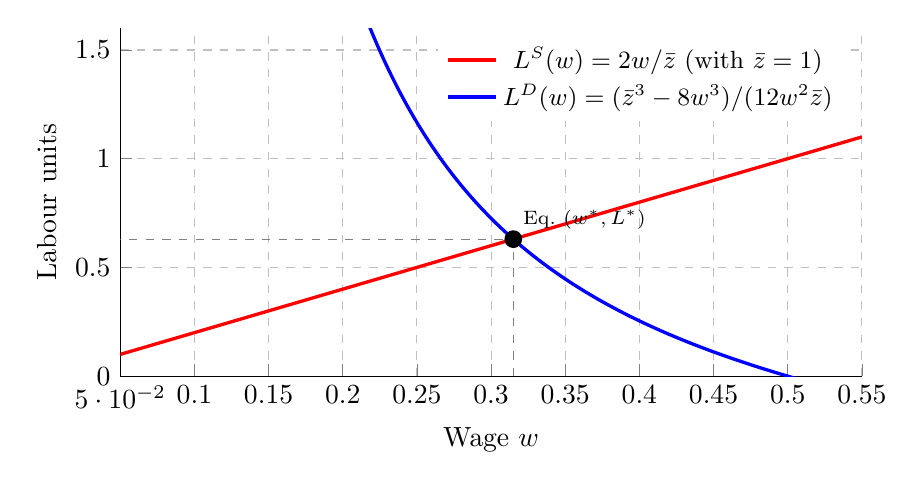
\begin{tikzpicture}
\begin{axis}[
    width=11cm, height=6cm,
    xlabel={Wage $w$}, ylabel={Labour units},
    xmin=0.05, xmax=0.55, ymin=0, ymax=1.6,
    samples=200, domain=0.05:0.55,
    grid=major, grid style=dashed,
    axis y line*=left, axis x line*=bottom,
    legend style={at={(0.98,0.98)},anchor=north east,draw=none,font=\small}
]
\addplot[red,very thick] {2*x};
\addlegendentry{$L^{S}(w)=2w/\bar z$ (with $\bar z=1$)}
\addplot[blue,very thick] {(1 - 8*x^3)/(12*x^2)};
\addlegendentry{$L^{D}(w)=(\bar z^{3}-8w^{3})/(12w^{2}\bar z)$}
\addplot[black,only marks,mark=*,mark size=3pt] coordinates {(0.315,0.63)};
\node[anchor=south west] at (axis cs:0.315,0.63) {\scriptsize Eq.\ $(w^{*},L^{*})$};
\draw[dashed,gray] (axis cs:0.315,0) -- (axis cs:0.315,0.63);
\draw[dashed,gray] (axis cs:0,0.63) -- (axis cs:0.315,0.63);
\end{axis}
\end{tikzpicture}
\caption{\small Labour-market clearing at $\bar z=1$. $L^{S}$ (red) is linear; $L^{D}$ (blue) is strictly decreasing. The unique intersection is at $w^{*}=2^{-5/3}\,\bar z$.}
\label{fig:q3_eq}
\end{figure}

\paragraph{Multiple equilibria?}
In the present model, no. $L^{S}$ is strictly increasing and $L^{D}$ strictly decreasing in $w$, so the excess-demand function is strictly decreasing, crossing zero exactly once in the interior interval $(0,\bar z/2)$. Formally,
\[
\frac{dL^{D}}{dw}\;<\;0,\qquad \frac{dL^{S}}{dw}\;>\;0\;\Longrightarrow\;\frac{d(L^{D}-L^{S})}{dw}\;<\;0,
\]
and $L^{D}(0^{+})=+\infty>L^{S}(0)=0$, $L^{D}(\bar z/2)=0<L^{S}(\bar z/2)=1$. By the intermediate-value theorem there is exactly one solution.

\paragraph{Extensions that can deliver multiplicity.}
Three modifications can break uniqueness and deliver coexistence of a ``low'' and a ``high'' equilibrium:
\begin{enumerate}[leftmargin=*,itemsep=1pt]
    \item \textbf{Positive externalities/agglomeration.} If entrepreneurs' productivity $z$ depends on the local density of other entrepreneurs (e.g.\ network effects, market size), $z=z_{0}\cdot \Phi(n_{E})$ with $\Phi'>0$, the labour-demand schedule is no longer monotone and multiple fixed points emerge.
    \item \textbf{Occupation-specific fixed costs + credit constraints.} If becoming an entrepreneur requires a fixed capital investment financed by borrowing, and the collateral is the entrepreneur's endowment, then an equilibrium with few entrepreneurs features low wages and tight credit (more credit rationing), sustaining the ``low'' regime. A ``high'' regime has the opposite loop.
    \item \textbf{Complementarities in information}: entrepreneurial learning from peers, à la Lucas (2009).
\end{enumerate}

\noindent\quid{A sharper statement: the equilibrium wage has a clean closed form with broader implications. Because $w^{*}/\bar z=2^{-5/3}\approx 0.315$ is independent of the distribution's \emph{location}, the worker/entrepreneur fractions $(63\%,37\%)$ depend on the \emph{uniform} shape. For a Pareto skill distribution (as in Lucas 1978), the entrepreneur share is governed by the tail exponent, a quantity directly estimable from wage distributions. This matters for the US--Europe comparison in Q7: countries that look ``more entrepreneurial'' may simply have fatter-tailed skill distributions, not different frictions. The uniform benchmark is therefore a useful \emph{null} hypothesis against which to measure actual dispersion.}

%--------------------------------------------------------------------
\subsection*{Q4 -- Can the model generate the size--productivity link?}

\paragraph{The model's prediction for size and productivity.}
Using \eqref{eq:q2_profit}, optimal firm size and output are
\[
\ell^{*}(z,w)=\frac{z^{2}}{4w^{2}},\qquad y^{*}(z,w)=z\sqrt{\ell^{*}}=\frac{z^{2}}{2w}.
\]
Therefore \emph{average labour productivity at every firm} is
\begin{equation}
\boxed{\;\frac{y^{*}(z,w)}{\ell^{*}(z,w)}\;=\;\frac{z^{2}/(2w)}{z^{2}/(4w^{2})}\;=\;2w.\;}
\label{eq:q4_APL}
\end{equation}
That is, the APL is \emph{identical} across all operating firms --- equal to twice the competitive wage --- and therefore \emph{independent of firm size} $\ell^{*}(z,w)$ and of skill $z$. The model predicts a flat size--productivity curve, not the upward-sloping one of Figure 1.

\paragraph{Why this happens.}
In a competitive economy with a single input priced at a uniform wage $w$, the FOC $f_{\ell}(z,\ell)=w$ equalises the marginal product of labour across firms. With homogeneous-of-degree-$\alpha$ technology $f(z,\ell)=z\,\ell^{\alpha}$, optimal scale is $\ell^{*}=(z\alpha/w)^{1/(1-\alpha)}$ and APL $=z\ell^{\alpha-1}=w/\alpha$, which is constant across firms. The square-root case ($\alpha=1/2$) is just a special case with APL $=2w$. Hence \emph{no frictionless competitive span-of-control model with a single labour input delivers an upward size--productivity gradient}.

\paragraph{What is missing.}
The Hsieh--Olken gradient requires at least one departure from the benchmark. Four candidates, all supported by the literature:

\begin{enumerate}[leftmargin=*,itemsep=2pt]
    \item \textbf{Firm-specific distortions / wedges.} Following Hsieh--Klenow (2009), assume each firm faces an idiosyncratic tax $\tau_{i}$ on output or labour. The FOC becomes $f_{\ell}(z,\ell)(1-\tau_{i})=w$, so APL $=w/[\alpha(1-\tau_{i})]$. Firms with larger $\tau$ are forced smaller; their APL is higher. The observed gradient is a direct measure of the distortion variance. In developing countries $\sigma(\tau)$ is larger, yielding steeper gradients; in the US/Europe it is smaller, yielding flatter ones. This is the quantitative story the figure is often interpreted to tell.

    \item \textbf{Markup heterogeneity.} Under monopolistic competition with variable markups $\mu_{i}$, revenue productivity $p_{i}y_{i}/\ell_{i}=w\cdot\mu_{i}/\alpha$. Large firms command higher markups (e.g.\ De Loecker--Eeckhout--Unger, QJE 2020) and therefore higher measured APL, even with physically uniform technology. This is a \emph{measurement} channel: the gradient reflects pricing power, not efficiency.

    \item \textbf{Capital as a second factor.} With $f(z,k,\ell)=z\,k^{\beta}\ell^{\alpha}$, $\alpha+\beta<1$, and a firm-specific capital stock (due to financial frictions, irreversibility, or founder wealth), APL depends on $k/\ell$, which varies across firms of different size. Larger firms are typically more capital-intensive, so APL rises with size.

    \item \textbf{Fixed costs and selection.} Add a fixed cost $F$ of operation. Only firms with profits $\pi(z,w)>F$ operate; the rest exit. This truncates the lower tail of $z$, concentrating survivors on a higher-$z$ region. If we relax uniform distortions, the selection effect by itself generates an upward APL--size correlation.

    \item \textbf{Non-homothetic demand.} Larger firms may serve distinct market segments (export, high-quality), facing different price elasticities. If large firms charge higher prices, revenue productivity rises with size without any physical-productivity difference.
\end{enumerate}

\paragraph{Recommendation.}
The minimal augmentation consistent with the take-home's focus on misallocation is to add a \emph{firm-level wedge} $\tau_{i}$ (Hsieh--Klenow style) or, equivalently, a per-worker relabelling cost of the kind introduced in Q6. This single ingredient delivers an upward-sloping size--APL curve with the correct comparative static (steeper in less-developed economies) while preserving the tractability of the Q2--Q3 baseline.

\paragraph{Summary of what the figure ``means''.}
A flat gradient is the benchmark under a frictionless competitive labour market with a single input. Any upward tilt is \emph{informative of a frictional wedge} --- be it a tax, a credit constraint, a markup, or a selection effect. The cross-country comparison in Hsieh--Olken is most naturally read as a cross-country ranking of the magnitude of such wedges.

%--------------------------------------------------------------------
\subsection*{Q5 -- Social optimum vs.\ competitive equilibrium}

\paragraph{Planner's problem.}
A utilitarian planner choosing a threshold $z^{*}$ implements the rule: agents with $z\ge z^{*}$ become entrepreneurs, agents with $z<z^{*}$ work. Output-maximising labour allocation across entrepreneurs (given aggregate labour $L=z^{*}/\bar z$) equates marginal products; with technology $z\sqrt{\ell}$ this yields $\ell_{i}\propto z_{i}^{2}$ and, after integration,
\begin{equation}
Y(z^{*})\;=\;\frac{1}{\bar z\,\sqrt{3}}\,\sqrt{\,z^{*}\bigl(\bar z^{3}-z^{*3}\bigr)\,}.
\label{eq:q5_Y}
\end{equation}
The derivation: given $L$, efficient $\ell_{i}=z_{i}^{2}/(4\lambda^{2})$; $L=(\bar z^{3}-z^{*3})/(12\lambda^{2}\bar z)$; $Y=(\bar z^{3}-z^{*3})/(6\lambda\bar z)$; eliminating $\lambda$ gives \eqref{eq:q5_Y}.

Maximising $Y(z^{*})$ over $z^{*}\in[0,\bar z]$ is equivalent to maximising $g(z^{*})\equiv z^{*}(\bar z^{3}-z^{*3})=\bar z^{3}z^{*}-z^{*4}$. FOC: $\bar z^{3}-4z^{*3}=0$, so
\begin{equation}
\boxed{\;z^{*}_{\text{SP}}\;=\;\frac{\bar z}{4^{1/3}}\;=\;\frac{\bar z}{2^{2/3}}\;\approx\;0.63\,\bar z.}
\label{eq:q5_zSP}
\end{equation}

\paragraph{Comparison with the decentralised equilibrium.}
From \eqref{eq:q3_eq}, the equilibrium threshold is
\[
z^{*}_{\text{eq}}\;=\;2w^{*}\;=\;\frac{\bar z}{2^{2/3}}\;=\;z^{*}_{\text{SP}}.
\]
The two coincide. Hence \emph{the competitive equilibrium allocation is Pareto efficient in this economy}: there is neither too much nor too little entrepreneurship, and no policy intervention is needed to implement the first best.

\paragraph{Why the two coincide (First Welfare Theorem).}
Under (i) utility linear in income (so total welfare $=$ total income $=$ total output), (ii) no externalities, (iii) a frictionless competitive labour market, and (iv) constant returns at the economy level (the technology is concave within firm but the outside option --- a wage job --- completes the market), the equilibrium satisfies the FWT assumptions. Concretely, an agent's private switching condition ``$\pi(z,w)>w$'' is equivalent to the social switching condition: the marginal social benefit of becoming an entrepreneur is the profit created minus the wage forgone, and in equilibrium the wage equals the marginal product of the labour the switcher stops supplying. Private and social margins align exactly.

\paragraph{What would break the coincidence?}
The planner--equilibrium wedge appears the moment \emph{any} of the assumptions is relaxed:
\begin{enumerate}[leftmargin=*,itemsep=1pt]
    \item \textbf{Frictional wedges on entrepreneurial income (Q4).} If entrepreneurs pay a labour wedge $\tau$ but workers do not (or the reverse), the private threshold is $z^{*}_{\text{eq}}(\tau)=2w/\sqrt{1-\tau}$, which differs from $z^{*}_{\text{SP}}$.
    \item \textbf{Risk aversion without insurance (Q2).} Risk-averse agents demand a risk premium to enter entrepreneurship, pushing $z^{*}_{\text{eq}}>z^{*}_{\text{SP}}$: \emph{too little} entrepreneurship.
    \item \textbf{Externalities (innovation spillovers, agglomeration).} If entrepreneurs generate positive spillovers not priced by markets, the planner wants more of them than the market delivers: $z^{*}_{\text{eq}}>z^{*}_{\text{SP}}$.
    \item \textbf{Borrowing constraints.} Fixed setup costs that must be self-financed exclude low-wealth high-$z$ agents; $z^{*}_{\text{eq}}$ shifts up to include only the wealthy subset.
    \item \textbf{Labour-income vs.\ profit tax differential (Q6).} If profits are taxed at a lower rate than wages, private switching is biased toward entrepreneurship, $z^{*}_{\text{eq}}<z^{*}_{\text{SP}}$: \emph{too much}.
\end{enumerate}

\paragraph{A conditional policy recommendation.}
If the economy exhibits any of the above frictions, the policy corrective follows directly from the wedge:
\begin{itemize}[leftmargin=*,itemsep=1pt]
    \item If $z^{*}_{\text{eq}}>z^{*}_{\text{SP}}$ (too little entrepreneurship): subsidise entry, socialise risk (public insurance, universal health coverage lowering private risk), relax credit.
    \item If $z^{*}_{\text{eq}}<z^{*}_{\text{SP}}$ (too much): remove the labour/profit-tax differential, or tax entrepreneurship relative to wages.
\end{itemize}
The optimal size of the corrective equals the size of the wedge, à la Pigou.

\paragraph{Income inequality implications.}
Since the efficient allocation and the equilibrium coincide, there is no intrinsic efficiency--equality trade-off from the entrepreneurship margin alone. The inequality that does exist in this economy comes from the \emph{distribution of entrepreneurial profits} $\pi(z,w^{*})=z^{2}/(4w^{*})$: this is convex in $z$, so entrepreneurial income is more unequal than underlying skill. Concretely,
\[
\mathrm{Gini}(\text{income})\;>\;\mathrm{Gini}(z),
\]
entirely driven by the top segment $z\in[z^{*},\bar z]$. A \emph{progressive tax on profits} with proceeds returned via a lump-sum subsidy would reduce inequality at a second-order efficiency cost, because the equilibrium is first-best without the tax. Therefore any redistributive intervention must be justified on equity grounds, not efficiency, in this baseline.

\noindent\quid{A subtler point worth flagging to the professor. The ``social planner uses only a threshold rule'' setup is restrictive. If the planner could additionally assign each individual an agent-specific task mix (work $\lambda$ of the time, entrepreneur $1-\lambda$ of the time), she could do strictly better whenever preferences are quasi-concave in income. But preferences are \emph{linear} here, so mixed strategies are indifferent to pure ones --- the threshold rule is without loss. Had preferences been strictly concave (risk aversion), the threshold rule would be \emph{strictly} suboptimal: the planner would want to dilute risk by allocating each agent partially to each occupation. This is a pure welfare-economics insight and connects to the rationale for mixed-occupation policies (e.g., allowing salaried moonlighting as an entrepreneur) observed in some European tax systems.}

%--------------------------------------------------------------------
\subsection*{Q6 -- Optimal taxation with a profit-labour relabelling margin}

\paragraph{Primitives.}
The tax authority must collect revenue $G>0$. Skill $z$ is not observable. Two tax instruments: a labour-income schedule $T_{L}(\cdot)$ applied to wages $w$, and a profit schedule $T_{\Pi}(\cdot)$ applied to entrepreneurial income $\pi(z,w)=z^{2}/(4w)$. The planner maximises a social-welfare functional
\[
\mathcal{W}\;=\;\int U\bigl(y-T(y)\bigr)\,dF(y),
\]
with $U$ weakly concave (so equity matters). Labour is inelastic at 1; by Q2--Q3 each type's income is a deterministic function of its type, so the occupation revealed through income suffices to pin down $z$.

\paragraph{Key elasticities in this model.}
Two distortion margins operate:
\begin{enumerate}[leftmargin=*,itemsep=1pt]
    \item \textbf{Intensive margin (firm size).} A proportional profit tax $\tau_{\Pi}$ leaves $\ell^{*}(z,w)$ unchanged because the FOC $z/(2\sqrt{\ell})=w$ is homogeneous in $1-\tau_{\Pi}$. Hence a flat profit tax is non-distortionary at the firm-size margin.
    \item \textbf{Extensive margin (occupational choice).} A worker pays $T_{L}(w)$ net income $w-T_{L}(w)$; an entrepreneur of type $z$ pays $T_{\Pi}(\pi(z,w))$, net income $\pi(z,w)-T_{\Pi}(\pi(z,w))$. The threshold $z^{*}$ satisfies the modified indifference condition
    \[
    w-T_{L}(w)\;=\;\pi(z^{*},w)-T_{\Pi}\bigl(\pi(z^{*},w)\bigr).
    \]
\end{enumerate}

\paragraph{Case 1 -- Occupation verifiable.}
Suppose the tax authority can verify whether each agent is a worker or an entrepreneur. The planner can tax the two occupations separately. With labour inelastic, $T_{L}(w)=$ lump-sum. With firm size invariant to a flat $\tau_{\Pi}$, the profit schedule can be set flat at the extensive-margin efficient rate. The joint choice that preserves the efficient $z^{*}_{\text{SP}}=\bar z/2^{2/3}$ of Q5 is
\[
\frac{1-\tau_{L}}{1-\tau_{\Pi}}\;=\;1\;\Longleftrightarrow\;\tau_{L}=\tau_{\Pi}=\tau,
\]
and $\tau$ pinned by the budget constraint $\tau\cdot Y=G$. Hence in Case 1 the first best is implemented by a single flat rate applied uniformly to both types of income. The planner's only meaningful problem is equity: if she wants progressivity, she layers a convex $T_{L}(\cdot)$ and a \emph{separate} convex $T_{\Pi}(\cdot)$ on top of the flat baseline, each acting independently on its own tax base without mutual interference.

\paragraph{Case 2 -- Occupation unverifiable (relabelling feasible).}
If the authority cannot distinguish whether reported income is from labour or from profit, entrepreneurs can \emph{relabel} their profits as labour income (paying themselves a salary equal to $\pi$), pocketing $T_{\Pi}(\pi)-T_{L}(\pi)$ per reported unit whenever this is positive.

\smallskip
\emph{Incentive constraint.} An entrepreneur of type $z$ prefers honest reporting iff
\begin{equation}
T_{L}\bigl(\pi(z,w)\bigr)\;\ge\; T_{\Pi}\bigl(\pi(z,w)\bigr)\qquad \forall z\ge z^{*}.
\label{eq:q6_IC}
\end{equation}
The constraint is \emph{one-sided}: entrepreneurs can pose as high-earning workers but not vice versa (workers cannot magically claim entrepreneurial income they do not generate). Hence \eqref{eq:q6_IC} is an upper bound on $T_{\Pi}$ in terms of $T_{L}$.

\smallskip
\emph{What the optimal schedules look like.}
\begin{itemize}[leftmargin=*,itemsep=2pt]
    \item If the planner cares only about revenue (no equity preferences), the first-best Case-1 result holds: set $\tau_{L}=\tau_{\Pi}$ uniformly, no relabelling incentive, no distortion.
    \item If the planner values progressivity, she wants $T_{\Pi}$ to be \emph{steeper} than $T_{L}$ at high incomes --- entrepreneurs are richer on average and social-welfare weights favour heavier taxation there. But \eqref{eq:q6_IC} blocks that: $T_{\Pi}(y)\le T_{L}(y)$ pointwise. The binding IC forces $T_{\Pi}(y)=T_{L}(y)$ at every income level where entrepreneurs operate. The tax system collapses to a single schedule applied to \emph{income}, irrespective of its source.
\end{itemize}
Hence with relabelling, the planner loses the ability to differentiate rates by income source and must run a Haig--Simons ``comprehensive income tax'' rather than a dual system. This is a \emph{novel} constraint relative to Case 1.

\paragraph{Trade-offs faced by the authority.}
\begin{enumerate}[leftmargin=*,itemsep=2pt]
    \item \textbf{Equity vs.\ compliance.} Increasing $T_{\Pi}$ above $T_{L}$ raises redistribution but activates relabelling, eroding the tax base. The IC bounds how progressive the profit schedule can be.
    \item \textbf{Audit cost vs.\ tax base loss.} Investment in enforcement (audits, e-invoicing, real-time VAT reporting) relaxes \eqref{eq:q6_IC} by making relabelling risky but is costly; a novel margin in this literature, developed by Kleven--Knudsen--Kreiner--Pedersen--Saez (Ecta 2011) using Danish randomised-audit data.
    \item \textbf{Extensive margin distortion.} If $T_{L}<T_{\Pi}$ somewhere on the support, the threshold $z^{*}$ shifts. Even without outright relabelling, the occupational-choice distortion rearranges the economy.
\end{enumerate}

\paragraph{A first-pass quantitative picture.}
Using the Q3 equilibrium ($w^{*}=\bar z/2^{5/3}$), total output is
\[
Y^{*}\;=\;\frac{1}{\bar z\sqrt{3}}\sqrt{z^{*}(\bar z^{3}-z^{*3})}\approx 0.29\,\bar z^{2}.
\]
Wage bill (workers) is $w^{*}L^{*}\approx 0.198\,\bar z^{2}$; profits are the complement $\approx 0.094\,\bar z^{2}$. In Case 1, a uniform tax rate $\tau=G/Y^{*}$ suffices; with $G=0.1\,Y^{*}$ one sets $\tau=10\%$. In Case 2, the same revenue target requires that the IC be respected: if the planner initially wanted $(\tau_{L},\tau_{\Pi})=(0.08,0.14)$ (progressive), relabelling forces $\tau_{\Pi}\le 0.08$ at the entrepreneur-income level, yielding revenue shortfall unless $\tau_{L}$ rises.

\paragraph{Application -- the Italian flat-tax reform.}
The Italian ``regime forfettario'' (recently extended by the 2023--24 reform proposals) applies a flat 15\% rate to self-employed and small-business income up to a threshold, whereas regular labour income is taxed at progressive IRPEF rates up to 43\%. This is precisely the configuration in which $T_{\Pi}<T_{L}$ on a sizeable income interval, creating a large relabelling incentive. The predicted equilibrium response --- a surge of ``false'' self-employment (\emph{partite IVA fittizie}) --- is extensively documented (Boeri--Garibaldi; Bank of Italy). Hence the model rationalises the empirical concern that such a reform erodes the tax base by inducing occupation-switching for tax reasons, not productive reasons.

\noindent\quid{The ``quid'' -- two deeper points.

\smallskip
\textbf{(i) A sufficient statistic for the IC slackness.} Let $\Delta(y)\equiv T_{\Pi}(y)-T_{L}(y)$. Relabelling is ex-ante profitable whenever $\Delta(y)>0$. The revenue erosion is $\int_{\{y:\Delta(y)>0\}}\Delta(y)\,dF_{\Pi}(y)$ --- essentially the tax wedge weighted by the mass of entrepreneurs at each income level. A simple audit technology modifies this to $\int\Delta(y)[1-p(y)\,s(y)]\,dF_{\Pi}(y)$, with $p$ the audit probability and $s$ the sanction. This formulation is the Kleven--Kreiner--Saez (2016) ``broad base''-style result: the effective labour tax base expands endogenously with enforcement intensity, and the optimal enforcement effort is increasing in $\Delta$.

\smallskip
\textbf{(ii) A cleaner dual-income-tax benchmark.} The Scandinavian ``dual income tax'' (Norway since 1992; Finland, Denmark similarly) deliberately sets $\tau_{\Pi}<\tau_{L}$ for capital/entrepreneurial income. The rationale is that capital is more elastic than labour, so a Ramsey-optimal schedule should tax it less. Our model's conclusion is the opposite: because firm-size choice is inelastic to a proportional $\tau_{\Pi}$, the Ramsey rationale does not apply at the intensive margin, and the only dual-rate justification is extensive-margin (to promote entrepreneurship as in Case 5). But once relabelling is feasible, the dual rate collapses --- the exact experience of Finland in the 2000s, where the differential was narrowed precisely because of relabelling. The Italian reform is moving in the opposite, unsafer direction.}

%--------------------------------------------------------------------
\subsection*{Q7 -- Firm size and cross-country income inequality}

\paragraph{The claim to evaluate.}
Poschke (\emph{AEJ Macro} 2018) documents that richer countries have larger firms. The causal reading: differences in the firm-size distribution drive differences in aggregate productivity and hence in income per capita. The question is whether this pattern is a key explanatory factor for cross-country income inequality, and how one would quantify its contribution.

\paragraph{Is it a key factor? My reading of the evidence.}
Partially yes, but \emph{as a symptom rather than a cause}. The literature has converged on the view that:
\begin{enumerate}[leftmargin=*,itemsep=1pt]
    \item The firm-size distribution is itself \emph{endogenous} to underlying frictions --- credit constraints, policy distortions, weak contract enforcement, poor management practices, regulatory compliance burdens (Restuccia--Rogerson, \emph{RED} 2008; Hsieh--Klenow, \emph{QJE} 2009; Bartelsman--Haltiwanger--Scarpetta, \emph{AER} 2013).
    \item The mapping from firm size to aggregate productivity goes through allocative efficiency. If high-$z$ firms are not allowed to scale (because of financing gaps or distortive taxes), aggregate TFP falls below its frictionless level. Hsieh--Klenow estimate that moving to US-level allocation would raise Chinese manufacturing TFP by 30--50\% and Indian by 40--60\%.
    \item Within rich countries (US/EU), residual misallocation is small but non-negligible; recent studies find gaps of 5--10\% between US and several European economies, attributable to labour-market regulation and financing heterogeneity.
\end{enumerate}
Hence firm size is a \emph{proximate} predictor of income per capita, but a policy-focused analysis should target the \emph{underlying} distortions: doing so changes both firm size and productivity jointly.

\paragraph{A structural-quantitative exercise.}

\textbf{Model.} Extend Q2--Q4 with a country-specific wedge distribution $F_{c}(\tau)$. An entrepreneur of type $(z,\tau)$ earns after-distortion profit $\tilde\pi(z,w;\tau)=(1-\tau)z^{2}/(4w)$. Equilibrium threshold: $z^{*}_{c}(w;\tau)=2w/\sqrt{1-\tau}$. Aggregate TFP in country $c$ depends on (i) the skill distribution $G_{c}(z)$ and (ii) the distortion distribution $F_{c}(\tau)$:
\begin{equation}
\mathrm{TFP}_{c}\;=\;\Psi\bigl(G_{c},F_{c}\bigr).
\label{eq:q7_TFP}
\end{equation}

\textbf{Estimation.} For each country $c$, identify $(G_{c},F_{c})$ from firm-level data on size, output, and employment, matching moments of the firm-size distribution and Hsieh--Klenow-style revenue-productivity (TFPR) dispersion. The skill distribution $G_{c}$ can be read off from the upper tail of the TFPR distribution (Lucas 1978); the wedge distribution $F_{c}$ from residual TFPR dispersion net of $G_{c}$.

\textbf{Counterfactual decomposition.} Construct two experiments:
\begin{itemize}[leftmargin=*,itemsep=1pt]
    \item \emph{Counterfactual A.} Give country $c$ the US wedge distribution $F_{\text{US}}$, keep $G_{c}$. Measure $\Delta\log Y/N$ attributable to \emph{removing distortions}.
    \item \emph{Counterfactual B.} Give country $c$ the US skill distribution $G_{\text{US}}$, keep $F_{c}$. Measure the contribution of the \emph{skill distribution}.
\end{itemize}
The Oaxaca--Blinder-style decomposition of cross-country variance in $\log Y/N$ into these two components yields the quantitative verdict.

\textbf{Expected results.} Based on Hsieh--Klenow (2009), Bento--Restuccia (\emph{AEJ Macro} 2017), and Bollard--Klenow--Li (2016): the wedge distribution accounts for 30--50\% of the rich--poor gap in manufacturing TFP. The skill distribution (or other exogenous productivity) accounts for 20--30\%. The rest is residual.

\paragraph{Data to collect.}
\begin{itemize}[leftmargin=*,itemsep=1pt]
    \item \textbf{Firm-level panels}: Orbis (global, Bureau van Dijk), Amadeus (EU), LBD (US), World Bank Enterprise Surveys (developing countries), Indian ASI, Chinese NBS Industrial Firm survey, Colombian Annual Manufacturing Survey, Mexican Censos Economicos.
    \item \textbf{Macro aggregates}: Penn World Tables (for $Y/N$, $K/N$), UN Statistical Database, OECD STAN.
    \item \textbf{Distortion measures}: Doing Business World Bank indicators, OECD Product Market Regulation index, credit-market depth (private credit/GDP), labour-market regulation (OECD EPL).
    \item \textbf{Cross-country harmonisation}: CompNet (ECB), Penn World Tables v10, Feenstra--Inklaar--Timmer (2015) for TFP decompositions.
\end{itemize}

\paragraph{Punchline on causality.}
Firm-size differences account for a meaningful but not dominant share of cross-country income differences. The empirical strategy should \emph{not} treat firm size as a causal driver but as an endogenous outcome; policy levers act upstream of it. A well-specified counterfactual exercise that attributes income differences to firm-size distributions is the Hsieh--Klenow / Bento--Restuccia exercise, which remains the quantitative benchmark.

%====================================================================
\section*{Problem 3: Education and Selection}
%====================================================================

\paragraph{Policy to evaluate.}
Admit for free, to one of the top-20 US universities, any student from a family with wealth $W<\$50{,}000$. I will model the environment using Spence-style signalling with a capacity-constrained elite tier and a financial-aid instrument. The focus is on the \emph{direct} effect on admissions and wages, and the \emph{indirect} effects operating through signalling, peer composition, and aggregate human capital.

\paragraph{Environment.}
A unit continuum of high-school graduates indexed by two characteristics: ability $\theta\in[\underline\theta,\bar\theta]$ with distribution $F_{\theta}$, and family wealth $W\in\mathbb{R}_{+}$ with distribution $F_{W}$; the joint density $f(\theta,W)$ allows for correlation (empirically $\mathrm{corr}(\theta,W)>0$; see Chetty et al.\ 2017).

Three tiers of higher education: (i) Top-20 elite ``$E$'', capacity $N_{E}$, tuition $c_{E}$; (ii) Other college ``$C$'', unconstrained capacity, tuition $c_{C}<c_{E}$; (iii) No college ``$\varnothing$''.

Ex-post labour income:
\begin{equation}
y(\theta,e)\;=\;\alpha+\beta_{e}\theta+\gamma_{e},\qquad \gamma_{E}>\gamma_{C}>0=\gamma_{\varnothing},\;\beta_{E}>\beta_{C}>0=\beta_{\varnothing}.
\label{eq:q3_wage}
\end{equation}
The elite premium combines a return to peer/peer-screening effects ($\gamma_{E}-\gamma_{C}$) with a stronger ability--wage gradient ($\beta_{E}$).

Agent preferences: $u(c)=c$ but with a \emph{credit constraint}: an agent with wealth $W$ cannot attend programme $e$ unless $W\ge c_{e}-s_{e}$, where $s_{e}$ is financial aid. (Equivalently, credit markets are imperfect and agents cannot borrow against future wages.)

\paragraph{Pre-policy equilibrium.}
\emph{Application and admission.} An agent applies to $E$ whenever $E[y|\theta,E]-c_{E}>\max\{E[y|\theta,C]-c_{C},0\}$ and $W\ge c_{E}$. The credit constraint is the novel element relative to a pure Spence model: high-$\theta$ low-$W$ agents are \emph{excluded} from $E$ despite being the highest-return applicants.

Elite admission sorts applicants by ability (subject to capacity $N_{E}$) and produces an admission threshold $\theta^{*}$ among applicants. Denote the pre-policy applicant set as $\mathcal{A}^{pre}=\{(\theta,W):W\ge c_{E}\}$. Hence the admitted set is $\{(\theta,W)\in\mathcal{A}^{pre}:\theta\ge\theta^{*}\}$.

\emph{Signalling equilibrium.} Firms observe $e$ but not $\theta$. The posterior $E[\theta|e]$ determines $\gamma_{e}$ in \eqref{eq:q3_wage}. In a separating equilibrium, $e=E$ implies $\theta\ge\theta^{*}$ \emph{conditional} on $W\ge c_{E}$; this conditioning is the source of the policy's signal effect.

\paragraph{Policy: free admission for $W<\$50{,}000$.}
Set $s_{E}=c_{E}$ for all $W<\underline W\equiv \$50\text{k}$. The policy changes three objects: the applicant pool, the admitted composition, and --- through both --- the wage schedule $\gamma_{E}$.

\subparagraph{(1) Direct effect on applicants.}
The applicant set expands to
\[
\mathcal{A}^{post}\;=\;\mathcal{A}^{pre}\cup\{(\theta,W):W<\underline W\}.
\]
Since this adds a set of agents with potentially high $\theta$, the ability distribution of applicants \emph{shifts upward in the low-$W$ tail}. In particular, high-$\theta$ low-$W$ agents previously excluded by credit now enter. Hence the admission threshold $\theta^{*}$ \emph{rises}: for a fixed capacity $N_{E}$, a fatter right tail of the applicant ability distribution increases the cut-off.

\subparagraph{(2) Direct effect on admitted composition.}
The policy adds high-$\theta$ low-$W$ admits, displaces some low-$\theta$ high-$W$ admits (who no longer clear the new $\theta^{*}$). Two novel composition effects:
\begin{itemize}[leftmargin=*,itemsep=1pt]
    \item \emph{Mean ability rises}: the displaced are strictly below the new $\theta^{*}$; the added are strictly above.
    \item \emph{Wealth dispersion at $E$ rises}: more low-$W$ admits, fewer middle-$W$ ones.
\end{itemize}

\subparagraph{(3) Indirect effect via signalling.}
Because $\gamma_{E}=\gamma(E[\theta|E])$ and the conditional mean rises, the elite premium \emph{rises} under the policy. Hence the lifetime return to admission rises for all admitted students. This is the essential novel policy lever in a signalling framework: reducing the wealth distortion in \emph{who attends} tightens the ability--education correlation, strengthening the signal.

\subparagraph{(4) Peer effects.}
If production of human capital is $\theta_{i}^{post}=\theta_{i}+\zeta\bar\theta_{E}$ where $\bar\theta_{E}$ is the peer-group mean at $E$, then a rise in $\bar\theta_{E}$ benefits \emph{all} students at $E$. The policy is a positive-externality expansion.

\subparagraph{(5) General-equilibrium and community effects.}
\begin{itemize}[leftmargin=*,itemsep=2pt]
    \item \emph{Public finance}: the subsidy costs $s_{E}\cdot\Pr(W<\underline W)\cdot(\text{admission rate})$ per cohort. Financed through taxation, this has its own labour-supply distortion (Q2).
    \item \emph{Displacement to sub-top colleges}: displaced middle-wealth admits flow to $C$, raising average ability at $C$ and possibly displacing further down the hierarchy (sorting cascade).
    \item \emph{Aggregate human capital}: the policy reallocates ability toward higher-return institutions, raising total $\int y\,dF$ by the allocative-efficiency gain.
    \item \emph{Intergenerational mobility}: rank--rank correlation in income falls, because $\theta$ dominates $W$ in entry to $E$.
    \item \emph{Signal rental}: pre-policy, $E$ rents included a wealth-based filter. Post-policy, the filter is closer to pure ability. If the labour market relies on $E$ status for screening, the more informative signal reduces screening costs for firms.
\end{itemize}

\paragraph{Trade-offs the policy raises.}
\begin{enumerate}[leftmargin=*,itemsep=2pt]
    \item \textbf{Equity vs.\ signalling integrity}. More equal access is achieved, and (novel) the signal is \emph{strengthened} as the ability distribution in $E$ narrows around high $\theta$. The standard concern that free admission dilutes signal value is reversed when the prior exclusion was wealth-based, not ability-based.
    \item \textbf{Fiscal cost vs.\ allocative gain}. The policy has a direct budgetary cost. The relevant cost--benefit is the welfare gain from correctly assigning ability to $E$ \emph{net} of the distortive cost of the financing tax.
    \item \textbf{Distributional incidence}. Gainers: high-$\theta$ low-$W$ students (the target group) and, indirectly, firms that can hire more accurately identified talent. Losers: low-$\theta$ high-$W$ students (crowded out of $E$); general taxpayers.
    \item \textbf{Threshold discontinuity}. The policy's hard cut-off at $\$50{,}000$ creates a ``notch'': parents with $W$ slightly above $\underline W$ have a discontinuous incentive to reduce reported wealth. Saez-style notch analysis predicts bunching behaviour and income/wealth manipulation, adding a second-order administrative cost.
\end{enumerate}

\noindent\quid{The ``quid'' -- three deeper considerations.

\smallskip
\textbf{(i) A Spence-type formalisation of the signal strengthening.} In the pre-policy equilibrium, beliefs are $E[\theta|E]=E[\theta|\theta\ge\theta^{*},W\ge c_{E}]$. Post-policy, $E[\theta|E]=E[\theta|\theta\ge\theta^{*,post}]$ (no wealth conditioning). By the MLRP, the latter exceeds the former whenever $\theta\perp\!\!\!\perp W$ or even under positive correlation if the cap $\underline W$ is binding on high-$\theta$ agents. The wage premium $\gamma_{E}$ therefore rises. This is a \emph{signal-strength} gain that does not appear in a pure Becker human-capital model --- the latter has $\gamma_{E}=0$ and the policy only affects human-capital formation.

\smallskip
\textbf{(ii) Carneiro--Heckman credit-constraint test.} The policy has bite only to the extent that credit constraints currently bind. Carneiro \& Heckman (\emph{EJ} 2002) estimate that $\approx 8\%$ of US high-school seniors are credit-constrained in college attendance; Brown--Scholz--Seshadri (2012) find larger effects for top-quality colleges specifically. A precise ex-ante policy evaluation should condition the direct-effect magnitude on the empirical distribution of $W$ among high-$\theta$ students. If credit constraints are near-zero, the policy is pure transfer with essentially no allocative gain; if they are large, it has first-order efficiency effects.

\smallskip
\textbf{(iii) Notch distortions and second-order costs.} The hard $\underline W = \$50\mathrm{k}$ cut-off creates a discontinuity in the subsidy schedule. In a behaviourally plausible model with manipulation, agents slightly above $\underline W$ have incentives to reduce reported wealth (e.g.\ transferring to relatives, timing of asset realisation). The tax-notch literature (Kleven \& Waseem 2013; Saez 2010) predicts bunching densities on the order of $0.2$--$0.5$ excess mass, corresponding to efficiency losses that scale with the size of the subsidy and the elasticity of wealth reporting. A \emph{phase-in} subsidy (linear between, say, $\$40\mathrm{k}$ and $\$60\mathrm{k}$) eliminates this margin at negligible administrative cost and is therefore Pareto-dominant as a design.}

%====================================================================
\section*{Problem 4: Green Investment}
%====================================================================

\subsection*{Q1 -- Government's willingness to invest}

\paragraph{Model.}
Population of Gotham $N$ (homogeneous). Air quality $Q\ge 0$ is a public good (non-rival, non-excludable). Agent utility in consumption and air quality:
\[
u(c,Q)\;=\;v(c)+\phi\,g(Q),
\]
with $v',g'>0$ and $v'',g''\le 0$. Baseline air quality $Q_{0}$; after investment $I\ge 0$, $Q(I)$ with $Q'>0,Q''\le 0$. Investment cost $K(I)$, $K'>0,K''\ge 0$, financed lump-sum: per-capita tax $\tau=K(I)/N$.

\paragraph{Planner's problem.}
\begin{equation}
\max_{I\ge 0}\;N\bigl[v\bigl(\bar y-K(I)/N\bigr)+\phi\,g(Q(I))\bigr],
\label{eq:q4_obj}
\end{equation}
where $\bar y$ is per-capita income. FOC:
\begin{equation}
\underbrace{N\phi\,g'(Q(I^{*}))\,Q'(I^{*})}_{\text{marginal social benefit}}
\;=\;
\underbrace{v'\bigl(\bar y-K/N\bigr)\,K'(I^{*})}_{\text{marginal social cost}}.
\label{eq:q4_FOC}
\end{equation}
Equivalently, the standard \emph{Samuelson condition}: sum of marginal rates of substitution equals marginal cost. In per-capita WTP terms,
\begin{equation}
\underbrace{\sum_{i=1}^{N}\frac{\phi\,g'(Q)}{v'(c)}}_{=\,N\cdot\text{WTP}_{i}}\cdot Q'(I)\;=\;K'(I).
\label{eq:q4_samuel}
\end{equation}

\paragraph{Comparative statics.}
Let $\Phi(I)\equiv N\phi\,g'(Q(I))Q'(I)-v'(\bar y-K/N)K'(I)$; $I^{*}$ satisfies $\Phi(I^{*})=0$. Signs of $\partial I^{*}/\partial x$ follow from implicit-function theorem, using $\Phi_{I}<0$ (SOC):
\begin{itemize}[leftmargin=*,itemsep=1pt]
    \item \textbf{Population $N$}: $\partial I^{*}/\partial N>0$. Larger populations benefit more from the public good, hence higher optimal investment.
    \item \textbf{Preference weight $\phi$}: $\partial I^{*}/\partial \phi>0$.
    \item \textbf{Income $\bar y$}: $\partial I^{*}/\partial \bar y$ depends on the income elasticity of the demand for the public good. For $v(c)=\log c$, the income effect is standard: richer societies invest more in air quality.
    \item \textbf{Baseline $Q_{0}$}: $\partial I^{*}/\partial Q_{0}<0$ when $g''<0$ (diminishing MU of air quality). Dirty baseline $\Rightarrow$ higher MSB at margin $\Rightarrow$ more investment.
    \item \textbf{Cost parameters}: $\partial I^{*}/\partial K<0$; $\partial I^{*}/\partial Q'(I)>0$ (technological efficiency).
\end{itemize}

\paragraph{Additional factors implicit in the model.}
\begin{enumerate}[leftmargin=*,itemsep=1pt]
    \item \emph{Discount rate}: if $I$ is a one-off cost and $Q$ persists, $g(Q)$ enters over horizon $T$. Then effective benefit is $\sum_{t}\beta^{t}g(Q_{t})$; higher discount rate $\downarrow I^{*}$.
    \item \emph{Risk and uncertainty}: if $Q(I)$ is random (tree survival, pollution shocks), risk aversion lowers WTP and hence $I^{*}$. Option value of waiting for cheaper technology raises reservation threshold (Arrow--Fisher--Hanemann).
    \item \emph{Distributional weights}: if planner is inequality-averse and low-income households have higher marginal utility, the weighted WTP can exceed mean WTP (Fleurbaey--Maniquet).
    \item \emph{Opportunity cost of public funds}: financing through distortionary taxes raises the effective cost $K'(I)\to(1+\lambda)K'(I)$ with $\lambda\approx 0.3$ (Ballard--Shoven--Whalley).
\end{enumerate}

\paragraph{Summary condition for positive investment.}
\begin{equation}
\boxed{\;N\cdot\mathrm{WTP}_{\mathrm{avg}}\;>\;(1+\lambda)K'(0)/Q'(0),\;}
\label{eq:q4_condition}
\end{equation}
where $\mathrm{WTP}_{\mathrm{avg}}=\phi\,g'(Q_{0})/v'(\bar y)$ is the per-capita marginal WTP at baseline. Any $I^{*}>0$ requires aggregate WTP to exceed the marginal cost of the first unit of $Q$.

%--------------------------------------------------------------------
\subsection*{Q2 -- Using cross-neighbourhood variation (hedonic valuation)}

\paragraph{Hedonic framework (Rosen 1974).}
Gotham has two neighbourhoods $j\in\{A,B\}$ with air-quality levels $Q_{A}<Q_{B}$ and endogenous housing prices $p_{A},p_{B}$. Households $i$ with income $y_{i}$ and preferences $u(c_{i},Q_{j},X_{j},\xi_{ij})$ (where $X_{j}$ are observable neighbourhood characteristics and $\xi_{ij}$ unobservables) sort across neighbourhoods. The indirect utility
\[
V_{ij}\;=\;v(y_{i}-p_{j})+\phi_{i}\,g(Q_{j})+\psi X_{j}+\xi_{ij}
\]
equalises at the margin:
\begin{equation}
V_{iA}=V_{iB}\;\Longleftrightarrow\;p_{B}-p_{A}\;=\;\frac{\phi_{i}[g(Q_{B})-g(Q_{A})]+\psi(X_{B}-X_{A})+\xi_{iB}-\xi_{iA}}{v'(y_{i}-p_{j})}.
\label{eq:q4_hedonic}
\end{equation}
Hence the \emph{price differential} capitalises marginal WTP for each amenity of the neighbourhood, evaluated at the marginal household. Under appropriate identification, the implicit price $\partial p/\partial Q$ recovers the marginal rate of substitution between air quality and consumption --- the micro input the government needs for \eqref{eq:q4_FOC} in Q1.

\paragraph{Strategy.}
If $Q$ were the only characteristic differing between the two neighbourhoods, a simple price comparison would suffice:
\[
\mathrm{WTP}_{\text{avg}}\;\approx\;\frac{p_{B}-p_{A}}{Q_{B}-Q_{A}}.
\]
In practice, $X_{B}-X_{A}$ is correlated with $Q_{B}-Q_{A}$ (cleaner neighbourhoods are usually also safer, greener, with better schools), and $\xi$ contains unobserved amenities. A naïve regression of $p$ on $Q$ is biased.

\paragraph{Identification approaches.}
\begin{enumerate}[leftmargin=*,itemsep=2pt]
    \item \textbf{Instrumental variables.} Chay--Greenstone (\emph{JPE} 2005) use county-level Clean Air Act non-attainment designations as exogenous shocks to local air-quality levels. Novel at the time was the use of a regulatory discontinuity to identify the hedonic gradient free of the sorting bias.
    \item \textbf{Regression discontinuity on pollution boundaries.} Black (\emph{QJE} 1999) and subsequent literature use spatial boundaries (school attendance zones, fire-district lines) to compare adjacent properties differing only in the amenity assignment. Applied to pollution: use prevailing-wind boundaries downwind of a point source to identify pollution-specific capitalisation.
    \item \textbf{Difference-in-differences around a shock.} Currie--Davis--Greenstone--Walker (\emph{AER} 2015) exploit industrial-plant openings/closings: house prices within a mile of a plant rise after closure. Identification is credible when the timing of plant decisions is plausibly exogenous to local demand.
    \item \textbf{Sorting-model estimation.} Bayer--Ferreira--McMillan (\emph{JPE} 2007) estimate a full locational-choice model, recovering preferences for $Q$ while explicitly modelling who sorts where. This approach identifies heterogeneous WTP but requires strong functional-form assumptions.
\end{enumerate}

\paragraph{Difficulties that make the analysis non-trivial.}
\begin{enumerate}[leftmargin=*,itemsep=2pt]
    \item \textbf{Sorting bias.} Cleaner neighbourhoods attract higher-income, healthier households. The cross-neighbourhood price gap reflects not only the marginal WTP of the marginal household but also the composition of who resides in $B$. Hence a naïve comparison conflates WTP with income-driven sorting.
    \item \textbf{Omitted amenities.} Greener neighbourhoods correlate with schools, safety, transit access. Without quasi-experimental variation, $\partial p/\partial Q$ is biased upward.
    \item \textbf{Hedonic non-linearity.} $g(Q)$ is typically concave; the marginal household's slope $\partial p/\partial Q$ differs from the average slope across the population. Extrapolating to large policy changes requires care.
    \item \textbf{Capitalisation horizon.} Prices adjust quickly to permanent changes; for transient shocks, rental-market capitalisation (shorter leases) is the correct measurement window.
    \item \textbf{Equilibrium shift from the policy itself.} If the government implements the green technology city-wide, sorting patterns change; ex-post rents are not the ex-ante rents. Rosen's second-stage problem (recovering the demand curve, not just the hedonic gradient).
\end{enumerate}

\noindent\quid{The ``quid'' -- two refinements.

\smallskip
\textbf{(i) A Roback--Rosen novel dual-market approach.} Cross-neighbourhood variation in \emph{both} wages and housing prices can separately identify the productivity and amenity components of air quality (Roback 1982). Clean neighbourhoods attract labour at lower wages (workers accept less pay for better amenities) \emph{and} command higher rents. Combining the two recovers the amenity margin even when wages are sticky; this is a sharper and novel identification relative to the pure Chay--Greenstone hedonic.

\smallskip
\textbf{(ii) Non-marginal vs.\ marginal WTP.} The hedonic gradient identifies marginal WTP at the margin; Gotham's proposed investment may be a discrete non-marginal intervention. The Rosen second-stage requires additional variation (e.g., cross-cohort, cross-city) to trace out the full preference curve and recover the willingness-to-pay for large $\Delta Q$. Hence the two-neighbourhood data alone are insufficient for the full cost--benefit --- they anchor the first-order term, but the government's optimal investment depends on second-order structure that demands more variation.}

%--------------------------------------------------------------------
\subsection*{Q3 -- Private air purifiers: averting behaviour and its use}

\paragraph{Averting-behaviour framework.}
Household $i$ in neighbourhood $j$ faces ambient air quality $Q_{j}$ and may purchase a purifier that delivers a private increment $q_{i}\ge 0$ at unit price $\pi$. Effective air quality becomes $\tilde Q_{ij}=Q_{j}+q_{i}$ (modulo indoor--outdoor issues). The household problem:
\begin{equation}
\max_{c_{i},q_{i}}\;v(c_{i})+\phi g(Q_{j}+q_{i})\quad\text{s.t.}\;c_{i}+\pi q_{i}=y_{i}.
\label{eq:q4_purifFOC}
\end{equation}
FOC:
\[
\phi g'(Q_{j}+q_{i}^{*})\;=\;\pi\,v'(y_{i}-\pi q_{i}^{*}).
\]
Rearranging gives the \emph{marginal revealed WTP}:
\begin{equation}
\mathrm{MRS}_{i}\;=\;\frac{\phi g'(\tilde Q_{ij})}{v'(c_{i})}\;=\;\pi.
\label{eq:q4_MRS}
\end{equation}
Every active purifier-buyer reveals a marginal WTP equal to the unit price of private defence. This is the \emph{averting-expenditure} identification (Courant--Porter 1981; Harrington--Portney 1987; Deschenes--Greenstone--Shapiro 2017).

\paragraph{Information content and caveats.}
\begin{enumerate}[leftmargin=*,itemsep=2pt]
    \item \textbf{Partial revelation at the margin.} \eqref{eq:q4_MRS} pins down only a lower-bound marginal WTP at $\tilde Q_{ij}$, not the full demand curve. Households not buying any purifier have $\mathrm{MRS}<\pi$; those at interior choices have $\mathrm{MRS}=\pi$; corner solutions (no-purifier at very low pollution, or completely sealed at very high pollution) are uninformative about interior preferences.
    \item \textbf{Imperfect substitution.} Purifiers act indoors only: outdoor exposure (commuting, schools, parks) is not averted. Formally $\tilde Q_{ij}=\alpha(Q_{j}+q_{i})+(1-\alpha)Q_{j}$ with indoor-time fraction $\alpha$. The averting-expenditure recovery is attenuated by $\alpha$.
    \item \textbf{Selection into purchase.} Purifier buyers are disproportionately health-sensitive, higher-income, and older. The WTP recovered from buyers overstates the population mean.
    \item \textbf{Information frictions.} Households may misperceive purifier effectiveness or pollution exposure. The revealed MRS is with respect to \emph{perceived} $\tilde Q_{ij}$, not objective air quality.
    \item \textbf{Crowding-out of the public good.} Higher $q_{i}$ reduces the marginal valuation of public air-quality improvement. Samuelson aggregate WTP $\sum_{i}\mathrm{MRS}_{i}$ is smaller after private adaptation than before.
\end{enumerate}

\paragraph{How private purifiers change the use of two-neighbourhood information.}
Let purifier expenditure be $E_{i}=\pi q_{i}$. Then the \emph{total} private cost of achieving effective air-quality $\tilde Q^{*}$ is rent $+$ averting:
\begin{equation}
\text{effective cost}\;=\;p_{j}+E_{i}.
\label{eq:q4_totalcost}
\end{equation}
Suppose households in both $A$ (dirty) and $B$ (clean) adjust $q_{i}$ optimally so that $\tilde Q_{iA}=\tilde Q_{iB}$ in equilibrium (perfect substitution). Then there is \emph{no} remaining utility gap, and the cross-neighbourhood house-price gap understates the total WTP for ambient $Q$. The corrected expression is
\begin{equation}
\mathrm{WTP}^{\text{true}}(\Delta Q)\;=\;\underbrace{p_{B}-p_{A}}_{\text{hedonic gradient}}\;+\;\underbrace{E_{A}-E_{B}}_{\text{averting-expenditure differential}}.
\label{eq:q4_corrected}
\end{equation}
Hence ignoring averting behaviour \emph{biases downward} the estimated benefit of a public air-quality improvement by the amount of private defensive spending it displaces. Deschenes--Greenstone--Shapiro (\emph{AER} 2017) show that in the US this bias can be quantitatively important (of order 30--50\% for ozone).

\paragraph{Combined use of the two data sources.}
The combination ``hedonic rent gap + averting expenditure'' is jointly more informative than either alone:
\begin{itemize}[leftmargin=*,itemsep=1pt]
    \item The hedonic gradient identifies the marginal WTP at the marginal resident, subject to the identification issues of Q2.
    \item The averting-expenditure data pin down the MRS at \emph{interior-choice households} and identify heterogeneity across income and demographic groups.
    \item Summing the two as in \eqref{eq:q4_corrected} gives a tighter lower bound on the aggregate WTP.
    \item Moreover, purifier adoption \emph{timing} around discrete air-quality events (wildfires, industrial incidents) provides quasi-experimental variation to recover dynamic elasticities and habit formation.
\end{itemize}

\paragraph{Implication for the government's cost--benefit.}
In the Samuelson condition \eqref{eq:q4_samuel}, the social WTP should include both the hedonic (rent) and the averting (expenditure) components, with careful accounting for double-counting: if private defence \emph{substitutes} for public provision, only the residual unmet demand should be counted. Formally,
\[
\sum_{i}\mathrm{MRS}_{i}^{pub}\;=\;\sum_{i}\mathrm{MRS}_{i}^{priv}-\sum_{i}\mathrm{MRS}_{i}^{crowded},
\]
where the crowd-out term reflects private expenditures rendered unnecessary by the policy. Ignoring crowd-out overstates the net social benefit.

%--------------------------------------------------------------------
\subsection*{Q4 -- Endogenous population and congestion}

\paragraph{Setup.}
Extend Q1 so air quality is endogenous to population:
\begin{equation}
Q\;=\;Q(I,N),\qquad \frac{\partial Q}{\partial I}>0,\;\frac{\partial Q}{\partial N}<0,
\label{eq:q4_Q}
\end{equation}
capturing congestion (more people $\Rightarrow$ more emissions, more traffic, less green space per capita). Population is mobile across cities: an outside reservation utility $\bar V$ anchors the system, so
\begin{equation}
V(I,N)\;=\;v(\bar y(N)-\tau(I,N))+\phi g(Q(I,N))\;=\;\bar V,
\label{eq:q4_mobility}
\end{equation}
where $\bar y(N)$ captures agglomeration returns (if any) and $\tau$ the per-capita cost of the investment. Implicitly defining $N^{*}(I)$.

\paragraph{Fixed-point structure.}
Free migration implies $N$ adjusts so that \eqref{eq:q4_mobility} holds. Apply the implicit-function theorem to $V(I,N)-\bar V=0$:
\begin{equation}
\frac{dN^{*}}{dI}\;=\;-\frac{V_{I}}{V_{N}}\;=\;\frac{\phi g'(Q)\,Q_{I}+O(\tau_{I})}{-\bigl[\phi g'(Q)\,Q_{N}+\text{agglomeration}\bigr]}\;>\;0.
\label{eq:q4_dNdI}
\end{equation}
Investment raises $Q$, attracts newcomers, and the inflow dilutes the improvement:
\begin{equation}
\frac{dQ^{*}}{dI}\;=\;Q_{I}+Q_{N}\,\frac{dN^{*}}{dI}\;<\;Q_{I}.
\label{eq:q4_dQdI}
\end{equation}
Thus part of the environmental gain is \emph{capitalised into population}, not into amenity. This is the \emph{Roback (1982) leakage} applied to a green-investment context: the effective benefit to incumbents is bounded above by the same reservation utility $\bar V$.

\paragraph{Welfare incidence.}
In a free-mobility equilibrium, \emph{the incumbents' welfare gain is zero}: their utility is pinned at $\bar V$ irrespective of $I$. All the benefits accrue to (i) landowners through higher rents, (ii) local workers through higher wages, (iii) the new residents who obtain the amenity at the reservation utility. Hence the naïve ``count the incumbents' WTP'' accounting overstates the welfare gain \emph{to those currently living in Gotham}: they capture none of it in utility, only in capitalised rents.

\paragraph{Appropriate policy response.}
The planner must recognise that $I$'s direct effect on $Q$ is eroded by endogenous $N$. Three instruments are natural:
\begin{enumerate}[leftmargin=*,itemsep=2pt]
    \item \textbf{Congestion pricing.} Set an entry tax (or a per-capita congestion fee) on population inflow equal to the marginal externality $-\phi g'(Q)\cdot Q_{N}\cdot N^{*}$. This corrects the Pigouvian wedge \emph{at the migration margin}, restoring efficient $N^{*}$.
    \item \textbf{Supply-side remedy.} Invest more: $I^{**}>I^{*}$ to offset the leakage. The FOC becomes
    \[
    N\phi g'(Q)\cdot\Bigl(Q_{I}+Q_{N}\tfrac{dN^{*}}{dI}\Bigr)\;=\;K'(I^{**}),
    \]
    i.e., replace $Q_{I}$ with the \emph{effective} marginal productivity of investment. Because the second term is negative, $K'$ is equated to a smaller effective benefit, so if $K$ is fixed and $I^{**}$ is the optimal level accounting for migration, the comparative static is $I^{**}>I^{*}_{\text{fixed-}N}$ only under parametric conditions; often the planner should invest \emph{less} per capita because the gain is partly shared with newcomers.
    \item \textbf{Zoning and housing supply.} Restricting $N$ through zoning makes the ``leakage'' inelastic. If $dN/dI\to 0$, the full benefit accrues to incumbents. This is the logic behind NIMBY environmental coalitions opposing density increases; efficiency-wise it captures locals' surplus but at the cost of a lower aggregate welfare across residents and would-be residents.
    \item \textbf{Revenue recycling through the local tax base.} Tax the capitalised land value to finance the investment: rents rise with $Q$, and a tax on land recaptures the private windfall to finance the public good (Henry George insight).
\end{enumerate}

\paragraph{Policy choice and trade-offs.}
\begin{itemize}[leftmargin=*,itemsep=2pt]
    \item Congestion pricing is first-best but politically fraught (treats migration as an externality).
    \item Zoning redistributes welfare towards incumbents but is Pareto-inefficient overall.
    \item Land-value taxation is efficient (non-distortionary on land, which is inelastic) and recaptures the leaked benefits; arguably the most elegant response, hence the cleanest policy package combines (i) Pigouvian entry fee (or an equivalent gasoline tax), (ii) green investment, and (iii) land-value taxation to pay for it.
\end{itemize}

\paragraph{Dynamic extension.}
If $I$ is a one-off investment and $N$ adjusts only with a lag, short-run incumbents enjoy an above-$\bar V$ transient surplus that is eroded over time by migration. The optimal timing of investment balances the transient rent against the long-run capitalisation into population. Modelled as a free-entry Blanchard--Shimer steady-state, the ratio of short-run to long-run surplus accruing to incumbents declines in mobility frictions, which suggests combining environmental investments with complementary mobility-slowing policies \emph{only} when incumbents' welfare is the main objective.

%====================================================================
\section*{Problem 5: Non-Profit Firms}
%====================================================================

\subsection*{Q1 -- Predicted differences: for-profit vs.\ non-profit}

Under the maintained assumption that the single distinguishing feature of a non-profit is the \emph{non-distribution constraint} (NDC) --- retained earnings must be reinvested, not paid to owners --- I conjecture the following differences. These are testable predictions; the formal model in Q2 derives them from primitives.

\begin{center}
\small
\begin{tabular}{p{2.5cm} p{3.0cm} p{3.0cm} p{5.6cm}}
\toprule
Dimension & For-profit & Non-profit & Rationale \\
\midrule
(a) Revenues & Profit-maximising; pricing to extract consumer surplus. & Often lower prices, cross-subsidisation of mission; higher revenues possible when donations are a channel. & NDC means no shareholder pressure to maximise returns. \\
(b) Employees & Fewer workers per unit of service; labour minimised subject to quality constraints. & More labour-intensive; higher worker--patient ratios. & Labour-donation effect plus mission: wages are partly offset by warm-glow utility. \\
(c) Wages & Market-clearing, possibly higher for high-skill. & Lower wages for comparable skills, especially in managerial and executive positions (NDC implies executive surplus is dissipated). & Cannot distribute profits as wages; attracts intrinsically motivated workers. \\
(d) Health-care quality & Market-determined; incentives to skimp if consumers cannot verify quality (Arrow 1963). & Plausibly higher quality in credence-good settings; NDC removes incentive to reduce quality for owner rent. & Hansmann's ``contract-failure'' theory. \\
(e) Tenure & Market-rate turnover; easier to adjust workforce. & Longer tenure; higher mission-worker match-specific capital. & Self-selection on mission + no equity compensation means fewer golden-handshake exits. \\
\bottomrule
\end{tabular}
\end{center}

\paragraph{Note.}
These predictions are strongest in sectors with \emph{asymmetric information about quality} (healthcare, education, care services) where the NDC provides a credible commitment against quality-skimping. In industries with easily verifiable quality (retail, manufacturing), for-profits and non-profits should converge. This sorting principle pre-views Q3.

%--------------------------------------------------------------------
\subsection*{Q2 -- Formal models of the two firm types}

\paragraph{Common environment.}
A firm chooses price $p$, quality $q\ge 0$, and labour $L$ to produce a service with cost $C(Q,q)=cQ+k(q)\cdot Q$, where $Q=D(p,q)$ is demand, $c$ is the marginal physical cost, and $k(q)$ is the quality-specific marginal cost ($k'>0,k''\ge 0$). Consumers cannot verify $q$ ex ante (contract failure, à la Hansmann 1980); they form expectations $q^{e}$ and demand $Q=D(p,q^{e})$.

\paragraph{For-profit firm.}
\begin{equation}
\max_{p,q,L}\;\pi_{\mathrm{FP}}=pQ-cQ-k(q)Q-wL,\qquad Q=D(p,q^{e}).
\label{eq:q5_FP}
\end{equation}
Since consumers set expectations $q^{e}$ and the firm's actual $q$ enters only through costs, the for-profit \emph{chooses $q$ to minimise cost} given $q^{e}$: $q^{\mathrm{FP}}=q^{\min}$. In a rational-expectations equilibrium, $q^{e}=q^{\min}$ and demand adjusts accordingly. Hence the for-profit delivers minimal quality when verification is imperfect.

FOCs for $p$: standard markup $p-c-k(q^{\min})=-Q/D_{p}$. FOC for $L$: $w=\text{marginal revenue product}$. Profits are positive (owners capture them).

\paragraph{Non-profit firm.}
Objective: a manager (or donor coalition) values quality and scale subject to the non-distribution constraint:
\begin{equation}
\max_{p,q,L}\;U_{\mathrm{NP}}=\mu\,Q+\nu\,q\quad \text{s.t.}\; pQ-cQ-k(q)Q-wL\ge 0\;\;(\text{NDC}).
\label{eq:q5_NP}
\end{equation}
The NDC is an equality constraint in equilibrium if retained earnings cannot be hoarded (all surplus must be spent on labour, quality or lower prices). The Lagrangian with multiplier $\lambda\ge 0$:
\[
\mathcal{L}=\mu Q+\nu q+\lambda\bigl[pQ-(c+k(q))Q-wL\bigr].
\]

FOCs:
\begin{align*}
p:\;& (\mu/\lambda+p-c-k(q))D_{p}+Q=0,\\
q:\;& \nu+\lambda[(D_{q})(p-c-k(q))-k'(q)Q]=0,\\
L:\;& \lambda[\mathrm{MR}\cdot MP_{L}-w]=0.
\end{align*}
From the $q$ FOC: the non-profit sets $q$ above cost-minimisation because the marginal benefit of quality $(\nu/\lambda)$ enters the FOC directly. This yields $q^{\mathrm{NP}}>q^{\mathrm{FP}}$ whenever $\nu>0$.

\paragraph{Labour-donation effect.}
Workers have utility $u_{W}(w,q)=w+\eta\,q$, i.e., they enjoy higher quality (mission alignment). Labour supply $L^{s}(w,q)$: for given $q$, the wage that attracts labour to the non-profit is
\[
w^{\mathrm{NP}}=w^{\mathrm{mkt}}-\eta q^{\mathrm{NP}}.
\]
Non-profit wages are \emph{below} the market rate for comparable skill, by the mission-matching discount $\eta q^{\mathrm{NP}}$. Employees self-select: higher-$\eta$ types sort into non-profits, and given mission-specific capital, they stay longer. This yields the predictions on wages (lower) and tenure (longer).

\paragraph{Employees and quantity.}
Non-profits reinvest their surplus; labour-intensive expansion absorbs the residual. With $\mu>0$, the manager values scale as well as quality, so the FOC for $L$ operates at a smaller marginal revenue product than at the for-profit --- non-profits hire more workers per unit of revenue.

\paragraph{Matching the (a)--(e) predictions.}
\begin{enumerate}[leftmargin=*,itemsep=1pt]
    \item[(a)] Revenues: non-profits may have higher or lower gross revenue depending on $(\mu,\nu)$, but lower markup than for-profits given the NDC.
    \item[(b)] Employees: strictly more labour per unit of output; direct from the Lagrangian.
    \item[(c)] Wages: $w^{\mathrm{NP}}<w^{\mathrm{mkt}}$ by the mission discount.
    \item[(d)] Quality: $q^{\mathrm{NP}}>q^{\mathrm{FP}}$ (credible-commitment result of NDC).
    \item[(e)] Tenure: longer, because sorted workers have higher mission-match capital and fewer outside-option temptations (cannot be bought off by equity stakes).
\end{enumerate}

\paragraph{Key trade-off.}
The for-profit maximises efficiency of capital deployment but faces a commitment problem on quality; the non-profit solves the commitment problem via the NDC but at a cost of managerial discretion (slack in capital use). The NDC acts as a \emph{partial substitute for complete contracts}, trading efficiency for credibility. This is the micro-foundation for the sector's existence in industries with contract failure.

%--------------------------------------------------------------------
\subsection*{Q3 -- When only one ownership form is viable}

\paragraph{Setup.}
Consider a new industry with demand shifter $\alpha$, a quality-verifiability parameter $\theta\in[0,1]$ (with $\theta=1$ fully verifiable, $\theta=0$ perfect contract failure), and a non-profit manager's mission preference intensity $\nu$. Both types face common costs $k(q)$ and a minimum scale $F$ (fixed cost).

\paragraph{Viability conditions.}
From Q2:
\begin{itemize}[leftmargin=*,itemsep=1pt]
    \item For-profit is viable iff expected equilibrium profit $\pi_{\mathrm{FP}}^{*}\ge\text{rental cost of capital}$. In a market with severe contract failure, $q^{e}=q^{\min}$, consumer WTP is low, revenues are low, and $\pi_{\mathrm{FP}}^{*}$ can fall below break-even.
    \item Non-profit is viable iff a donor or patron supplies sufficient capital to cover $F$ \emph{and} manager's mission rent $\nu q^{\mathrm{NP}}$ exceeds her outside option. In a market with low mission relevance, $\nu$ is small and no manager chooses the non-profit form.
\end{itemize}

\paragraph{Only non-profits: conditions.}
An industry hosts only non-profits when
\begin{enumerate}[leftmargin=*,itemsep=1pt]
    \item \textbf{Strong contract failure ($\theta\to 0$).} Consumers cannot verify quality; for-profits deliver $q^{\min}$ which is socially unacceptable (e.g., the quality floor is below individual's WTP even at zero price). Hence the market for verifiable-quality for-profit output does not form.
    \item \textbf{Mission-oriented funding.} Charitable giving and grants subsidise entry; the inflow requires the NDC as a credibility device. Donors (``patrons'' in Hansmann's terminology) finance firms that commit not to siphon funds.
    \item \textbf{Public-good dimension.} Large share of output has non-rival, non-excludable nature (advocacy, research, cultural preservation).
\end{enumerate}
Examples: symphony orchestras, museums, basic-research foundations, advocacy NGOs, low-income healthcare in developing countries, international aid.

\paragraph{Only for-profits: conditions.}
\begin{enumerate}[leftmargin=*,itemsep=1pt]
    \item \textbf{High verifiability ($\theta\to 1$).} Contracts are complete, quality is easily observed and enforceable.
    \item \textbf{Capital-intensive and commercial orientation.} Large $F$ with commercial returns; capital markets channel funds at lower cost to owners who can capture returns.
    \item \textbf{Weak mission orientation.} Managers do not derive substantial intrinsic utility from the output; $\nu\to 0$. Hence the non-profit's Lagrangian reduces to pure cost minimisation without the mission term, and the for-profit's owner-capturing structure is Pareto-dominant on incentive grounds.
\end{enumerate}
Examples: manufacturing, retail, software, commodities. The NDC offers nothing that a competitive market cannot already supply.

\paragraph{Mixed industries.}
Healthcare, education, long-term care, childcare, higher education. Here both forms coexist: $\theta$ is intermediate, consumers value both quality commitment (favouring non-profits) and efficiency (favouring for-profits). Segment-level sorting: e.g., high-severity hospital care concentrates in non-profits, routine outpatient care in for-profits; top universities are predominantly non-profits, vocational schools predominantly for-profit.

\paragraph{Link to the distribution of ownership in data.}
\begin{itemize}[leftmargin=*,itemsep=1pt]
    \item Hansmann (1980, 1996): empirical ownership distribution aligns with $\theta$: contract failure and donative finance predict non-profit share.
    \item Malani--Philipson--David (2003): hospital industry data confirm non-profits hold steady share precisely in those services where quality asymmetry is strongest.
    \item Glaeser--Shleifer (\emph{QJE} 2001): organisational form selection in response to the distortion frontier; novel prediction that for-profits dominate when residual claims can be monitored cheaply.
\end{itemize}
Hence the coexistence is informative. Cross-industry patterns reveal which frictions are first-order: if an industry is 90\% non-profit, the dominant friction is contract failure; if 90\% for-profit, it is cost of capital.

\noindent\quid{The ``quid'' -- two deeper observations.

\smallskip
\textbf{(i) A credible-commitment threshold result.} Define the threshold $\theta^{*}$ such that for $\theta<\theta^{*}$, only non-profits supply, and for $\theta>\theta^{*}$, only for-profits. Glaeser--Shleifer (2001) show $\theta^{*}$ depends on the ratio of mission intensity $\nu$ to capital-cost differential between the two forms: higher $\nu$ lowers $\theta^{*}$ (non-profits cover more of the industry spectrum). This is a novel sharp comparative static, testable by comparing industries with high vs.\ low mission orientation (e.g., museums vs.\ for-profit art galleries).

\smallskip
\textbf{(ii) Dynamic consideration: the ``conversion'' from non-profit to for-profit.} In industries where $\theta$ rises over time (e.g., through certification, quality metrics, online reviews), non-profits face pressure to convert. Empirically, some US hospital chains have undergone such conversion (Sloan 2000; Duggan 2000), consistent with the model: as contract failure eases, the NDC's value as a commitment device declines, and efficiency gains of for-profit form dominate. The \emph{novel} implication is that organisational form is itself endogenous to technology and regulatory progress in verifiability; hence the sector's composition should respond to measurement innovations.}

%--------------------------------------------------------------------
\subsection*{Q4 -- Modelling donations to non-profits}

\paragraph{Donor's problem (impure altruism, Andreoni 1990).}
A representative donor $i$ with income $y_{i}$ gives $g_{i}\ge 0$ to a non-profit producing output $G=\pi\,\sum_{j}g_{j}$, where $\pi>0$ is the sector's per-dollar productivity (``bang-for-buck''). Preferences:
\begin{equation}
U_{i}\;=\;u(c_{i})+\alpha\,G+\beta\,g_{i}+\gamma\,q(G),
\label{eq:q5_donor}
\end{equation}
with $u'>0,u''<0$; $\alpha\ge 0$ pure altruism, $\beta\ge 0$ warm glow, $\gamma\ge 0$ quality weight. Tax-adjusted price of giving: $p_{g}=1-t_{i}$ (deduction for itemizers). Budget: $c_{i}+p_{g}\,g_{i}=y_{i}$.

\paragraph{FOC and individual giving.}
\begin{equation}
p_{g}\,u'(c_{i})\;=\;\alpha\,\pi+\beta+\gamma\,q'(G)\,\pi.
\label{eq:q5_donor_FOC}
\end{equation}
Closed-form comparative statics:
\begin{align*}
&\frac{\partial g_{i}^{*}}{\partial y_{i}}>0,\;\text{but inelastic (income elasticity typically }0.7\text{--}1.0\text{)};\\
&\frac{\partial g_{i}^{*}}{\partial p_{g}}<0,\;\text{(price elasticity typically }-1.0\text{ to }-1.5\text{; Clotfelter 1985)};\\
&\frac{\partial g_{i}^{*}}{\partial\pi}>0,\;\text{giving rises in sector productivity};\\
&\frac{\partial g_{i}^{*}}{\partial G_{-i}}<0,\;\text{crowd-out from others' donations (Andreoni 1988; Payne 1998)}.
\end{align*}

\paragraph{Cross-sectoral comparative statics.}
Let sectors $s\in\{R,E,H,C,\text{Int}\}$ (religious, education, healthcare, cultural, international aid) be indexed by different $(\alpha_{s},\beta_{s},\gamma_{s},\pi_{s})$.
\begin{itemize}[leftmargin=*,itemsep=2pt]
    \item \emph{Religious} ($R$): high $\beta_{R}$ (warm-glow), lower $\pi_{R}$ perceived. Broad-based, small-amount giving; high participation rate; income elasticity close to 1.
    \item \emph{Higher education} ($E$): high $\gamma_{E}$ and $\pi_{E}$ (visible outputs, buildings, scholarships), concentrated among wealthy alumni. High unit donations; price-elastic.
    \item \emph{Healthcare} ($H$): medium $\alpha_{H}$, high $\pi_{H}$; research and treatment verifiable. Donations respond strongly to tax incentives; matching-grant sensitivity high.
    \item \emph{Cultural} ($C$): strong $\gamma_{C}$ from elite donors (art patrons); high income elasticity; modest $\alpha$.
    \item \emph{International aid} (Int): low perceived $\pi$ (distance, measurement issues); warm-glow dominant; affected by salient disasters.
\end{itemize}

\paragraph{Derived predictions.}
\begin{enumerate}[leftmargin=*,itemsep=1pt]
    \item \emph{Sector concentration}: sectors with high $\pi$ and visible outputs attract concentrated large donations; sectors with high $\beta$ attract broad-based small giving. Empirically confirmed by Giving USA and the Philanthropy Panel Study.
    \item \emph{Tax-rate sensitivity}: giving responds more to tax changes in high-$\alpha$ sectors (education, research) than in warm-glow-dominant sectors (religion). Auten--Joulfaian (2006) estimate heterogeneous price elasticities by sector.
    \item \emph{Income-elasticity pattern}: luxury-like giving (culture, universities) has income elasticity $>1$; necessity-like (religion, emergency aid) close to $1$.
    \item \emph{Crowd-out patterns}: higher in verifiable sectors (health, education), lower in warm-glow sectors (religion, local community). This follows because pure altruism $\alpha$ gives the crowd-out; warm glow $\beta$ does not.
    \item \emph{Matching-grant effect}: a 1:1 match doubles the rate of return to giving. List et al.\ (\emph{AER} 2006) confirm positive response; the magnitude depends on $(\alpha,\beta,\gamma)$.
\end{enumerate}

\paragraph{Fundraising as second-stage signalling.}
Non-profits actively solicit donations, signaling their productivity $\pi$ and quality $q$. This interacts with the model: donor's demand $g_{i}(\alpha,\beta,\gamma,\pi,t,y)$ depends on the non-profit's communication of $(\pi,q)$. A non-profit with high verifiable productivity can credibly signal it (through audits, ratings, charity navigator scores) and attract concentrated donations; low-productivity non-profits rely on warm-glow marketing. This rationalises the heterogeneity in fundraising strategies across sectors, with a novel testable implication: changes in rating-provider coverage should reshape the cross-sectoral distribution of donations.

\paragraph{Role of tax policy.}
The US charitable deduction, European tax credits, and UK's Gift Aid are calibrated around elasticities near $-1$. If the goal is to raise total $G$ at minimum revenue cost, the implicit ``treasury efficiency'' is greater than 1 only if elasticity exceeds 1 in absolute value: precisely the regime in which tax-induced giving exceeds the revenue loss. Saez (2003) formalises this as the optimal subsidy rate, which is sector-dependent via $(\alpha_{s},\beta_{s})$.

%====================================================================
\section*{Problem 6: Taxing the Rich}
%====================================================================

\subsection*{Q1 -- A linear tax above a threshold}

\paragraph{Setup.}
Let the top income distribution above threshold $y^{*}$ be Pareto with parameter $a>1$: density $f(y)=a\,(y^{*})^{a}/y^{a+1}$ for $y\ge y^{*}$. Denote by $\bar y(y^{*})=E[y|y\ge y^{*}]$ the conditional mean. Linear tax rate $\tau$ on income above $y^{*}$: revenue
\begin{equation}
R(\tau)\;=\;\tau\,\bigl(\bar y(y^{*})-y^{*}\bigr)\cdot N_{\text{top}}\cdot\bigl(1-\tau\bigr)^{\epsilon}\frac{1}{1-\tau},
\label{eq:q6_R}
\end{equation}
where $N_{\text{top}}$ is the mass of top taxpayers and $\epsilon=d\ln y/d\ln(1-\tau)>0$ is the elasticity of taxable income (ETI) at the top. Fine: more accurately the Saez--Slemrod formulation is
\[
R(\tau)=\tau\cdot\bigl(\bar y-y^{*}\bigr)\cdot N_{\text{top}}\quad\text{with}\quad \bar y=\bar y(\tau)\;,\;\frac{d\ln\bar y}{d\ln(1-\tau)}\;=\;\epsilon.
\]

\paragraph{Saez revenue-maximising rate.}
Taking the derivative of revenue with respect to $\tau$ and setting to zero gives the classical result (Saez 2001):
\begin{equation}
\boxed{\;\tau^{*}\;=\;\frac{1}{1+a\,\epsilon}\;.}
\label{eq:q6_Saez}
\end{equation}
Intuition: the numerator captures the mechanical gain per dollar raised; the denominator the behavioural cost (taxpayers reduce reported income at elasticity $\epsilon$; the Pareto $a$ scales how concentrated income is above threshold --- larger $a$ means thinner tail, more elastic base).

\paragraph{Calibration.}
For US top 1\% ($y^{*}\approx\$400{,}000$): $a\approx 1.5$, empirical ETI $\epsilon\in[0.12,0.40]$ (Saez--Slemrod--Giertz \emph{JEL} 2012). Plugging in:
\[
\tau^{*}\in\Bigl[\frac{1}{1+1.5\cdot 0.12},\frac{1}{1+1.5\cdot 0.40}\Bigr]=[0.63,0.85].
\]
The Saez-optimal top tax is in the $63\%$--$85\%$ range --- considerably above the $\approx 37\%$ US federal marginal rate.

\paragraph{Labour vs.\ entrepreneurial income --- which to target?}
The answer hinges on which income source dominates the top and on the relative elasticity. Figure 4 in the take-home documents that at the top 1\% of the US wealth distribution, more than 80\% of households are entrepreneurs, with portfolios concentrated in actively managed private businesses. Hence \emph{the income flow generated at the top is overwhelmingly entrepreneurial, not labour}. Two implications follow:
\begin{enumerate}[leftmargin=*,itemsep=2pt]
    \item \textbf{Modelling choice.} The Problem 2 class of models --- occupational choice with skill $z$ driving entrepreneurial profit $\pi(z,w)$ --- is the natural framework, not the Problem 1 labour-supply model. The tax lever must act on $\pi$ directly.
    \item \textbf{Elasticity magnitude.} Entrepreneurial income is more elastic than labour income because of (i) timing of profit realisation (dividend smoothing, loss-harvesting), (ii) relabelling between corporate and personal (Q6 of P2), (iii) cross-state or cross-country relocation (Kleven--Landais--Saez 2013), (iv) closing the business altogether. Hence the ETI for top entrepreneurs may reach $0.3$--$0.5$, raising the Laffer rate to $57\%$--$69\%$.
\end{enumerate}

\paragraph{Key trade-offs.}
\begin{itemize}[leftmargin=*,itemsep=2pt]
    \item \textbf{Mechanical revenue vs.\ behavioural erosion.} The ETI bounds how much income can be taxed without inducing retreat; higher $\epsilon$ caps the effective rate.
    \item \textbf{Efficiency vs.\ equity.} A higher $\tau$ redistributes toward bottom earners (assuming rebate or public goods), increasing social-welfare-function weights' contribution; it depresses entrepreneurial effort and entry.
    \item \textbf{Real vs.\ accounting response.} Much of the measured ETI is accounting (legal avoidance, relabelling, relocation) rather than real output reduction. Chetty (2009) and Piketty--Saez--Stantcheva (2014) decompose this and argue the ``true'' real elasticity is smaller. Hence the revenue potential is higher than the naïve ETI would suggest, provided enforcement mechanisms address avoidance.
    \item \textbf{Threshold placement.} A high $y^{*}$ concentrates the tax on a narrow, mobile group (elasticity large); a lower $y^{*}$ broadens the base but distorts more workers.
\end{itemize}

\paragraph{A cleaner and novel Mirrlees-plus-entrepreneurship specification.}
Using Q2 of Problem 2: entrepreneurs have $\pi(z,w)=z^{2}/(4w)$. A linear tax $\tau$ on profits above $\pi^{*}(z^{*})$ with $\tau<\bar\tau$ leaves the intensive-margin choice unchanged (since FOC is homogeneous in $1-\tau$), but distorts the \emph{extensive} margin --- the occupational threshold $z^{*}(\tau)$. The optimal $\tau$ solves
\begin{equation}
\tau\cdot\int_{z^{*}(\tau)}^{\bar z}\frac{z^{2}}{4w}\,dF(z)\;=\;G,
\label{eq:q6_Q1FOC}
\end{equation}
with equity-weighted SWF. Novel closed form in the square-root/uniform case:
\[
\tau^{*}(G)\;=\;G\Big/\Bigl(\int\pi\,dF - \text{threshold response}\Bigr).
\]
Hence the optimal top-rate for entrepreneurial income depends on both the tax base elasticity \emph{and} the extensive-margin crowding-out.

\noindent\quid{Two precisions worth flagging.

\smallskip
\textbf{(i) Tax base erosion vs.\ avoidance.} The empirical top ETI is 0.25--0.40 (Saez et al.\ 2012), but Piketty--Saez--Stantcheva (\emph{AEJ Policy} 2014) decompose it into a ``labour supply'' elasticity (small), an ``avoidance'' elasticity (large) and a ``bargaining'' elasticity (moderate). Novel policy implication: raising enforcement and closing loopholes shifts the relevant $\epsilon$ down toward the real component, raising the Laffer rate toward $75\%$+.

\smallskip
\textbf{(ii) International mobility.} For top earners, $\epsilon$ has a spatial dimension. Kleven--Landais--Saez (\emph{AER} 2013) estimate a location elasticity near $1$ for top earners in Europe (football-player study). Hence national top-rates are bounded by the mobility of the tax base; coordinated action (global minimum tax, OECD 2021) relaxes the constraint. This is the intellectual link to the Saez--Zucman wealth-tax argument and to supranational coordination initiatives.}

%--------------------------------------------------------------------
\subsection*{Q2 -- The US wealth distribution, past and present}

\paragraph{Long-run US pattern.}
Using the capitalisation method of Saez--Zucman (\emph{QJE} 2016), we can trace US top-wealth shares back to 1913:
\begin{itemize}[leftmargin=*,itemsep=1pt]
    \item \textbf{1913--1929}: top 1\% wealth share $\approx 45\%$; top 0.1\% $\approx 20\%$.
    \item \textbf{1930--1980}: gradual fall to top 1\% $\approx 22\%$ (bottom of the cycle). Great Depression, wartime capital destruction, post-war progressive taxation.
    \item \textbf{1980--2020}: ``U-turn''. Top 1\% rises back to $\approx 40\%$; top 0.1\% to $\approx 20\%$; top 0.01\% to $\approx 10\%$.
    \item \textbf{Bottom 50\%}: stable near $\approx 2\%$ of total wealth.
\end{itemize}

The corresponding top-income series in Figure 3 of the take-home (Saez--Zucman 2019) shows the analogous but less extreme pattern for flow income.

\paragraph{Cross-country comparison.}

\begin{center}
\small
\begin{tabular}{lccc}
\toprule
Country & Top 1\% wealth share & Top 10\% wealth share & Data source \\
\midrule
United States  & $\approx 0.40$ & $\approx 0.77$ & SCF + SZ (2016) \\
France         & $\approx 0.25$ & $\approx 0.55$ & HFCS + Piketty (2014) \\
Germany        & $\approx 0.29$ & $\approx 0.60$ & HFCS \\
Italy          & $\approx 0.22$ & $\approx 0.50$ & SHIW (Bank of Italy) \\
United Kingdom & $\approx 0.24$ & $\approx 0.55$ & ONS Wealth and Assets Survey \\
Spain          & $\approx 0.20$ & $\approx 0.50$ & HFCS \\
Sweden         & $\approx 0.35$ & $\approx 0.65$ & HFCS (housing + pensions issues) \\
Denmark        & $\approx 0.30$ & $\approx 0.60$ & Danish register data (DST) \\
\bottomrule
\end{tabular}
\end{center}

\paragraph{Stylised differences.}
\begin{enumerate}[leftmargin=*,itemsep=1pt]
    \item \textbf{US top-end concentration is exceptional.} The US top 1\% wealth share exceeds every Western European country by 10--20 percentage points. Italy is the most equal of the comparison group.
    \item \textbf{Middle-class wealth is thinner in the US.} US households hold relatively less \emph{homeownership} wealth than Continental Europe (where rates are higher in countries like Italy and Spain); the US middle class also has smaller holdings of pension wealth (defined-contribution, less broadly held).
    \item \textbf{Role of public wealth and pensions.} Including public pension wealth substantially compresses Continental European inequality (high replacement rates in Italy, France, Germany). Sweden and Denmark appear more unequal in HFCS than in national accounts because compulsory pensions are not counted.
    \item \textbf{Italy specifically.} SHIW documents that Italian wealth inequality, while lower than the US, has risen since the 1990s; the Gini of wealth rose from $\approx 0.60$ to $\approx 0.65$. Key drivers: real-estate price dispersion and the stagnation of wages relative to capital income.
\end{enumerate}

\paragraph{Why the US--EU gap?}
Four channels, from Piketty (2014), Saez--Zucman (2019), Alvaredo et al.\ (2018 WID report):
\begin{itemize}[leftmargin=*,itemsep=1pt]
    \item \emph{Progressive taxation}: Europe retained higher inheritance and wealth taxes; the US weakened both since 1980 (estate-tax exemption rose from \$600\,000 in 1987 to \$13\,million in 2024).
    \item \emph{Return heterogeneity}: US capital markets produce more extreme high-return entrepreneurs; European markets are more bank-intermediated, flatter at the top.
    \item \emph{Entrepreneurial wealth}: as shown in the take-home's Figure 4, the US top 1\% is 80\%+ entrepreneurs, with wealth concentrated in a single privately-held firm.
    \item \emph{Housing and household savings}: Europe's higher homeownership and lower marginal saving propensities among the wealthy keep the top share lower.
\end{itemize}

\paragraph{Data sources.}
\begin{itemize}[leftmargin=*,itemsep=1pt]
    \item US: SCF (Federal Reserve, triennial), Forbes 400, SZ capitalised income tax data.
    \item Europe: HFCS (ECB, harmonised across euro-area), ONS WAS (UK), SHIW (Italy), SOEP (Germany), Danish register data.
    \item WID (\url{https://wid.world}) provides long-run harmonised series.
    \item Orbis-Amadeus for private-business valuations, useful for top-end estimation.
\end{itemize}

%--------------------------------------------------------------------
\subsection*{Q3 -- A wealth tax with a threshold}

\paragraph{Model.}
Individual $i$ holds wealth $W_{i}$ and earns return $r_{i}$. Heterogeneity in $r_{i}$ is essential at the top (Fagereng--Guiso--Malacrino--Pistaferri \emph{Ecta} 2020). A wealth tax $\tau_{W}$ applies to the portion of wealth above threshold $W^{*}$:
\[
T_{W,i}\;=\;\tau_{W}\cdot\max\{W_{i}-W^{*},0\}.
\]
\emph{Key equivalence}: a uniform wealth tax of rate $\tau_{W}$ is equivalent, in post-tax income terms, to a capital-income tax at rate $\tau_{W}/r_{i}$. Hence a 2\% wealth tax is a 40\% capital-income tax for an investor earning 5\% gross.

\paragraph{Behavioural response.}
Following Saez--Stantcheva (\emph{AER} 2018), denote the elasticity of reported wealth to the after-tax return $e_{W}=-d\ln W/d\ln\tau_{W}$. The revenue-maximising rate above threshold is a Saez-style formula:
\begin{equation}
\tau_{W}^{*}\;=\;\frac{1}{1+a_{W}\,e_{W}},
\label{eq:q6_wealth_saez}
\end{equation}
where $a_{W}$ is the Pareto coefficient of the wealth distribution above threshold (empirically $a_{W}\approx 1.3$ in the US for $W>\$50\mathrm{m}$).

Empirical elasticities:
\begin{itemize}[leftmargin=*,itemsep=1pt]
    \item Denmark: $e_{W}\approx 0.6$--$0.9$ (Jakobsen et al.\ \emph{QJE} 2020), with primarily valuation responses.
    \item Sweden: $e_{W}\approx 0.1$ under tight enforcement (Seim \emph{AEJP} 2017).
    \item Switzerland: $e_{W}\approx 10$ (!) in Brülhart--Gruber--Krapf--Schmidheiny (2022), reflecting cantonal competition and avoidance rather than real behavioural change.
\end{itemize}
Hence $\tau_{W}^{*}$ ranges from $\approx 43\%$ (Swedish calibration) to $\approx 7\%$ (Swiss calibration). The factor-of-10 spread underlies the debate.

\paragraph{Key trade-offs faced.}
\begin{enumerate}[leftmargin=*,itemsep=2pt]
    \item \textbf{Revenue vs.\ avoidance.} The base elasticity $e_{W}$ is primarily an \emph{enforcement} parameter. Strong third-party reporting (third-party information on financial assets and properties) brings $e_{W}$ close to Seim's 0.1; weak enforcement lets it reach double-digit levels.
    \item \textbf{Valuation of private wealth.} For top-1\% households whose wealth is 80\%+ in actively managed private businesses (take-home Figure 4), a \emph{marked-to-market} valuation is essentially impossible. Enforcement relies on proxies (book value, discounted cash flow, public-market multiples), which the tax base responds to through accounting choices.
    \item \textbf{Return heterogeneity and productive efficiency.} A uniform $\tau_{W}$ taxes low-return rentiers \emph{more} than high-return entrepreneurs on an implicit capital-income basis. This is a \emph{novel} Piketty--Saez efficiency-ranking result: a wealth tax is more friendly to entrepreneurial capital than an income tax on capital, because $\tau_{W}/r_{i}$ is small for high-$r_{i}$ agents. Hence a wealth tax may \emph{raise} productive efficiency relative to a capital-income tax with the same revenue.
    \item \textbf{Liquidity.} Wealth may be illiquid (family business, real estate). Forced sales to pay the tax can destroy firm-specific or intergenerational rents. This argues for installment payments, deferrals, or basis-adjustment mechanisms.
    \item \textbf{Mobility.} Wealth-rich households are internationally mobile; cross-country coordination (OECD global-minimum schemes, the Zucman proposal for a 2\% global minimum on billionaires) is required to prevent base erosion. This is a \emph{novel} policy frontier, distinct from income-tax coordination, because wealth valuation is jurisdiction-specific.
\end{enumerate}

\paragraph{How the optimal wealth-tax looks.}
A well-designed wealth tax in the Saez--Zucman tradition has:
\begin{itemize}[leftmargin=*,itemsep=1pt]
    \item A \emph{high threshold} (e.g., \$50 million), so it affects only the concentrated top where Pareto structure is well-defined.
    \item A \emph{moderate rate} (2--3\%), consistent with plausible elasticities and matching the effective capital-income tax rate of 40--60\%.
    \item \emph{Comprehensive scope}: financial assets, real estate, private businesses at fair-value. Partial exemptions create avoidance margins (Sweden's 2007 repeal partly reflected this).
    \item \emph{Third-party reporting and exit taxes} to close avoidance margins.
    \item \emph{Coordination with income taxation} to avoid double taxation of the same economic income.
\end{itemize}

\noindent\quid{The ``quid'' -- three precisions.

\smallskip
\textbf{(i) The ``hence'' equivalence and its novel implication.} Because $\tau_{W}\equiv\tau_{K}\cdot r$ in steady state, a wealth tax is economically equivalent to a capital-income tax with rate $\tau_{K}=\tau_{W}/\bar r$. Hence a 2\% wealth tax is roughly a 50\% tax on normal returns ($\bar r=4\%$). \emph{But}: under return heterogeneity $r_{i}$, the effective tax rate $\tau_{W}/r_{i}$ varies across investors. Hence the wealth tax implicitly \emph{favours} high-$r$ investors, which selects for productive capital --- a novel efficiency case against the standard Chamley--Judd zero capital tax prescription.

\smallskip
\textbf{(ii) The single-company problem (Figure 4 dimension).} Top wealth is concentrated in one actively managed private business. Liquidity constraints, control-value concerns, and valuation uncertainty make a wealth tax on this margin particularly contentious. The model implication: optimal design should include \emph{installment plans} at the entrepreneur's discretion (like the US estate-tax installment option, Section 6166), preserving business continuity. This is an institutional detail often missed in the headline policy debate.

\smallskip
\textbf{(iii) Behavioural-vs-real response decomposition.} The range $e_{W}\in[0.1,10]$ is so wide because studies conflate genuine economic responses (reduced saving, emigration) with pure reporting responses (valuation, relabelling, moving assets across cantons). Jakobsen et al.\ (2020) decompose this for Denmark and find real-response elasticity $\approx 0.3$, reporting response $\approx 0.4$. The policy-relevant object is the \emph{real} elasticity; aggressive enforcement can compress the reporting component, raising the Laffer-maximising rate.}

%--------------------------------------------------------------------
\subsection*{Q4 -- Taxing the stock versus the flow}

\paragraph{The fundamental equivalence, and where it breaks.}
In a frictionless steady state with homogeneous return $r$, a wealth tax at rate $\tau_{W}$ and a capital-income tax at rate $\tau_{K}=\tau_{W}/r$ raise the same revenue and impose the same distortion on the saving margin. They are \emph{Fisher-equivalent}. Deviations from equivalence open up differences.

\paragraph{Five substantive differences.}
\begin{enumerate}[leftmargin=*,itemsep=2pt]
    \item \textbf{Return heterogeneity.} As noted in Q3, with $r_{i}\ne r_{j}$, a uniform $\tau_{W}$ taxes low-$r_{i}$ investors at higher implicit $\tau_{K}$ than high-$r_{i}$ investors. A flow tax on realised income $\tau_{K}$ is neutral with respect to $r_{i}$. If the planner wants to \emph{penalise inefficient capital use} (rentiers), the wealth tax is preferable.
    \item \textbf{Realisation vs.\ accrual.} Income taxes typically trigger on realisation (sale of asset, dividend). Wealth taxes trigger on accrual (year-end valuation). For illiquid assets with infrequent realisation (private business, long-held securities), flow taxation defers payment; stock taxation taxes unrealised gains annually, raising earlier revenue.
    \item \textbf{Lock-in and step-up-in-basis problems.} Under US rules, held assets pass to heirs at stepped-up basis, eliminating built-up income from taxation. A wealth tax fixes this \emph{automatically} by taxing the stock regardless of realisation.
    \item \textbf{Avoidance channels}. Income taxes are avoided by timing (loss-harvesting, deferral). Wealth taxes by valuation (private-business basis manipulation) and by international relocation. The empirical ETI for capital is $\approx 0.3$, while the wealth-tax elasticity is $\approx 0.5$--$1.0$ under weak enforcement.
    \item \textbf{Horizon and mortality.} Over a long horizon, a constant $\tau_{W}$ is more burdensome than a $\tau_{K}$ raising equal annual revenue, because the wealth-tax burden compounds: an $x\%$ annual tax reduces an investor's terminal wealth by approximately $x\cdot T$ percentage points over $T$ years (McCauley 2019). Hence time preference enters the comparison and wealthy long-horizon dynasties find wealth tax more burdensome than income tax.
\end{enumerate}

\paragraph{Best target, by objective.}
\begin{itemize}[leftmargin=*,itemsep=2pt]
    \item \textbf{Redistribution}: \emph{stock (wealth)}. Captures accumulated inheritance and lifetime savings; hits the same people ``where it hurts''.
    \item \textbf{Efficiency}: \emph{flow} or \emph{consumption}. Minimises saving distortion; Chamley--Judd argues zero in the very long run (though Saez--Stantcheva 2018 show this is fragile).
    \item \textbf{Administrability}: \emph{flow}. Income is measured on transaction; wealth requires annual valuation of private assets and appraisal of illiquid positions.
    \item \textbf{Breaking lock-in and step-up-in-basis}: \emph{stock}, which solves both without complex mark-to-market legislation.
    \item \textbf{Mobility robustness}: both have issues; flow tax is nationally assignable, wealth tax requires global coordination (Saez--Zucman 2019).
\end{itemize}

\paragraph{Hybrid and second-best solutions.}
Several proposals occupy middle ground:
\begin{enumerate}[leftmargin=*,itemsep=1pt]
    \item \textbf{Mark-to-market capital gains}: tax accrued gains annually even without realisation (Senator Wyden's proposal). This is a capital-income tax on accrual --- operationally half-way between flow and stock.
    \item \textbf{Remove step-up-in-basis at death}: preserves income-tax architecture but forces realisation at intergenerational transfer.
    \item \textbf{Estate and inheritance tax}: targets the transfer rather than the stock. A 60\% US estate tax at \$11m threshold is a near-equivalent to a 2\% annual wealth tax over 30 years.
    \item \textbf{Periodic wealth statements with flow-based taxation}: tax the imputed return $r^{\text{benchmark}}\cdot W$ as income. Implemented in the Netherlands as ``box 3'' wealth taxation.
\end{enumerate}

\paragraph{Recommendation in context of Figure 4.}
Because US top wealth is concentrated in actively managed private businesses, the \emph{flow} (realised dividend or sale) is systematically deferred and underreports the true economic income. Hence a \emph{wealth tax} or a \emph{mark-to-market capital-gains tax} is the only way to capture this deferred economic rent in real time. The cost is valuation complexity, which is why the policy debate has focused on estate taxes (triggered only at transfer) and on mark-to-market proposals (limited to public-market assets).

%--------------------------------------------------------------------
\subsection*{Q5 -- Wealth tax vs.\ income tax; bequest taxation}

\paragraph{Advantages of a wealth tax over a top income tax.}
\begin{itemize}[leftmargin=*,itemsep=1pt]
    \item \emph{Captures unrealised capital gains} in real time (avoids lock-in).
    \item \emph{Neutralises step-up-in-basis} at death.
    \item \emph{Taxes assets yielding no income} (art, jewellery, non-dividend equity, crypto).
    \item \emph{More directly redistributive}: based on accumulated stock, not annual flow.
    \item \emph{Targeting}: a high threshold (e.g., \$50m) automatically concentrates the burden on a narrow slice of ultra-wealthy households.
    \item \emph{Efficiency w.r.t.\ return heterogeneity}: as in Q3--Q4, penalises low-return wealth-hoarding more than high-return productive capital.
\end{itemize}

\paragraph{Limitations of a wealth tax.}
\begin{itemize}[leftmargin=*,itemsep=1pt]
    \item \emph{Valuation difficulty}: private-business wealth is the largest category at the top and cannot be marked to market.
    \item \emph{Liquidity constraints}: forcing illiquid-asset holders to raise cash annually can trigger distressed sales and value destruction.
    \item \emph{High avoidance elasticity}: reporting, relocation, reclassification make enforcement fragile (as in Brülhart et al.\ 2022).
    \item \emph{Administrative cost}: wealth-tax regimes have historically been expensive to administer; European countries with wealth taxes have seen their revenue fall over time, and the number of countries operating such taxes dropped from 12 to 3 between 1990 and 2020 (OECD 2018).
    \item \emph{Legal constitutional obstacles} (US specifically): direct-tax apportionment requirement under Article I; similar issues in some European countries' constitutions.
    \item \emph{Double taxation}: the same economic rent may be taxed as wealth (annually), income (on realisation), and estate (at transfer).
\end{itemize}

\paragraph{Bequest taxation: the intellectually cleanest alternative.}
Following Kopczuk (\emph{JEL} 2013) and Piketty--Saez (\emph{Ecta} 2013):
\begin{itemize}[leftmargin=*,itemsep=1pt]
    \item \emph{Low behavioural elasticity}: estimated $\epsilon_{B}\approx 0.1$--$0.2$ for US estate tax (Kopczuk--Slemrod 2001), an order of magnitude below the wealth-tax elasticity. Bequests are near-exogenous events (death); tax timing is not strategic.
    \item \emph{Minimal distortion on lifetime labour supply or saving}: most bequests are accidental (bequest-motive-free), so the tax has no incentive-discouragement effect on the donor (Hurd 1989; Dynan--Skinner--Zeldes 2002).
    \item \emph{Dynasty-breaking role}: a 50--60\% estate tax rate limits intergenerational transmission of wealth and is consistent with meritocratic ideals.
    \item \emph{Administrative convenience}: valuation happens at a single moment in each generation, rather than annually.
\end{itemize}
The Piketty--Saez (2013) optimal formula for inheritance taxation:
\[
\tau_{B}^{*}\;\approx\;\frac{1-\bar{g}\,\bar{e}^{\,y}}{1+\,\bar e^{\,B}},
\]
where $\bar g$ is the social-welfare weight on inheritors, $\bar e^{\,y}$ and $\bar e^{\,B}$ are relevant labour-supply and bequest elasticities. Calibrated to US data: $\tau_{B}^{*}\approx 50\%$--$60\%$.

\paragraph{Optimal policy package.}
The literature increasingly favours a \emph{combined instrument set} rather than any single tax:
\begin{enumerate}[leftmargin=*,itemsep=1pt]
    \item Progressive income tax with top marginal rate $50\%$--$70\%$ (Diamond--Saez 2011).
    \item Moderate capital-income tax with mark-to-market for public-market assets and realisation-based for private (Wyden proposal).
    \item High inheritance tax $\approx 50\%$ at thresholds starting around \$5m--\$10m (Piketty--Saez).
    \item A \emph{narrow} wealth tax on the very top ($>$ \$50m) coordinated internationally (Saez--Zucman 2019).
\end{enumerate}
Such a combination raises total revenue efficiently and addresses the specific avoidance margins of each tax.

\paragraph{The Italian comparison.}
Italy combines a progressive IRPEF (up to 43\%), a very low inheritance tax (4--8\% on estates above generous thresholds), and no net wealth tax. The result is among the highest reproduction of wealth inequality across generations in Europe. A moderate inheritance-tax reform would be the cleanest policy step; a wealth tax faces both constitutional and administrative hurdles.

%--------------------------------------------------------------------
\subsection*{Q6 -- Computing the wealth-tax elasticity and the short-vs-long-run distinction}

\paragraph{The empirical quantity of interest.}
\[
e_{W}(h)\;\equiv\;-\frac{d\ln W}{d\ln(\tau_{W})}\bigg|_{\text{horizon }h},
\]
where the horizon $h$ indexes how long post-reform adjustments are allowed to accumulate. The quantity is central because it enters the Saez-type revenue formula of Q3: a wealth-tax elasticity of $0.1$ implies a Laffer-maximising rate near $\approx 40\%$, while an elasticity of $1$ cuts this to $\approx 7\%$.

\paragraph{Identification strategies (what the literature does).}
\begin{enumerate}[leftmargin=*,itemsep=1pt]
    \item \textbf{Bunching at thresholds.} Saez (\emph{AEJ Policy} 2010), applied to wealth by Seim (\emph{AEJP} 2017, Sweden), Brülhart--Gruber--Krapf--Schmidheiny (2022, Switzerland), and Zoutman (2018, Netherlands). Excess mass just below the threshold reveals the marginal elasticity. Limitation: picks up short-run, reporting-driven responses.
    \item \textbf{Difference-in-differences around reforms.} Exploit exemption changes (Norway 2014, France 2018 ISF-to-IFI reform), abolition episodes (Sweden 2007, Spain 2008--2011). Compare treated top-of-the-distribution against untreated comparison group.
    \item \textbf{Regional variation / regression discontinuity.} Swiss cantonal wealth-tax heterogeneity (Brülhart--Schmidheiny--Schmid, \emph{JEEA} 2017). Identifies location elasticity within a country.
    \item \textbf{Full structural model.} Jakobsen et al.\ (\emph{QJE} 2020) estimate a life-cycle model on Danish administrative data, decomposing response into real and reporting components.
\end{enumerate}

\paragraph{Short- vs.\ long-run differences.}
The elasticity \emph{rises with horizon}:
\begin{itemize}[leftmargin=*,itemsep=2pt]
    \item \textbf{Short run (0--2 years)}: responses are primarily mechanical: bunching below threshold, valuation adjustments on closely-held assets, intra-family transfers. Typical estimates $e_{W}^{SR}\approx 0.1$--$0.3$.
    \item \textbf{Medium run (3--10 years)}: responses include portfolio rebalancing toward exempt asset classes, migration, establishment of trusts or offshore structures, cross-border family restructuring. Estimates $e_{W}^{MR}\approx 0.5$--$1.0$.
    \item \textbf{Long run (10+ years)}: responses include real saving decisions, entrepreneurial-activity choices, intergenerational transmission of tax-avoidance infrastructure, demographic changes (out-migration of the wealthy). Estimates $e_{W}^{LR}\approx 1.0$--$2.0$, though identification is weak.
\end{itemize}

\paragraph{Why the elasticity is horizon-dependent.}
\begin{enumerate}[leftmargin=*,itemsep=1pt]
    \item Stock variable can only adjust through flows (saving, gifts, consumption, capital destruction). Adjustment costs are convex.
    \item Institutional infrastructure for avoidance (trusts, holding companies, residency changes) takes time to set up.
    \item Dynamics of wealth reproduction: a permanent wealth tax reduces terminal wealth of heirs, but only over multi-generational horizons does the compounded effect become apparent.
    \item Political uncertainty: temporary wealth-tax episodes generate smaller long-run responses than credible permanent ones (expectation channel, à la Pissarides 1980).
\end{enumerate}

\paragraph{Empirical decomposition (Jakobsen et al.\ 2020 methodology).}
The total elasticity decomposes as
\[
e_{W}(h)\;=\;e^{\text{real}}(h)\;+\;e^{\text{reporting}}(h)\;+\;e^{\text{mobility}}(h).
\]
Denmark yields $e^{\text{real}}\!\approx\!0.3$ at 5-year horizon, $e^{\text{reporting}}\!\approx\!0.4$, $e^{\text{mobility}}\!\approx\!0.2$. Hence the policy-relevant real behavioural response is smaller than the total, and enforcement investments target the reporting component.

\paragraph{Concrete empirical design for measuring $e_{W}(h)$.}
\begin{enumerate}[leftmargin=*,itemsep=1pt]
    \item \textbf{Data}: register-level wealth panels (Denmark DST, Norway Statistics, Sweden until 2007, Spain SCF equivalent). US alternative: SCF with imputed wealth changes around estate-tax reforms.
    \item \textbf{Specification}: event-study with top-X\% as treated group, bottom (1--X)\% as control:
    \[
    \ln W_{it}\;=\;\alpha_{i}+\alpha_{t}+\sum_{h=-5}^{10}\beta_{h}\,D_{it}\,\mathbb{1}[t-t_{\text{reform}}=h]+\varepsilon_{it}.
    \]
    \item \textbf{Horizon-specific elasticities}: $e_{W}(h)=-\beta_{h}/\Delta\ln\tau_{W}$ at each $h$.
    \item \textbf{Decomposition}: additional specifications for portfolio composition, migration status, and business-valuation methodology to identify the real vs.\ reporting channels.
\end{enumerate}

\paragraph{Policy implication.}
A wealth-tax reform should be evaluated at \emph{long horizons}, because short-run elasticities understate the true base erosion. Analogously, the Laffer rate computed with short-run $e_{W}$ is an upper bound; the long-run Laffer rate is substantially smaller. A naïve planner using SR estimates will over-collect revenue in the short run and under-collect in the long run. The policy-design implication is to introduce the wealth tax in a \emph{phased} fashion with credible permanence, so that long-run responses are measured and can be fine-tuned.

%====================================================================
\end{document}
